%% --------------------------------------------------
%% CHAPTER: Cellular Automaton
%% --------------------------------------------------
\chapter{A Cellular Automaton for Track Reconstruction}\label{chapter:CellularAutomaton}

\section{Cellular Automata}
A \acf{CA} is a \ac{FSM} which usually consists of a regular grid of cells in a finite number of dimensions, each of which exists in one of a finite number of states. A neighbourhood is defined to be some region around any given cell, and the next generation is formed by updating the state of each cell according to a fixed rule which takes into account the current cell state as well as the state of its neighbours. Typically, this rule is identical for each cell and at each time step. The update rule is usually applied simultaneously to the whole grid.

The concept was originally devised by John von Neumann~\citep{vonNeumann1966} in the 1940s as a method of creating self-reproducing machines using a \ac{CA} with 29 states. Cellular automata became popular in the 1970s with the development of the \emph{Game of Life} by John Conway (see, for example, \citep{Gardner1970}). In \emph{Life}, cells exist in one of two states (live or dead) and the neighbourhood is defined to be the 8 cells surrounding a central cell on a square grid. The update rules are simple but result in varied and complex behaviour. Figure \ref{fig:ca_life_four_steps} illustrates these rules for the first four states of a simple initial pattern.

\begin{enumerate}
\item Any live cell with $< 2$ live neighbours dies (under-population).
\item Any live cell with 2 or 3 live neighbours lives on.
\item Any live cell with $> 3$ live neighbours dies (over-population).
\item Any dead cell with exactly 2 live neighbours becomes live (reproduction).
\end{enumerate}

\begin{figure}
\centering
\subfigure[Step 1]{
	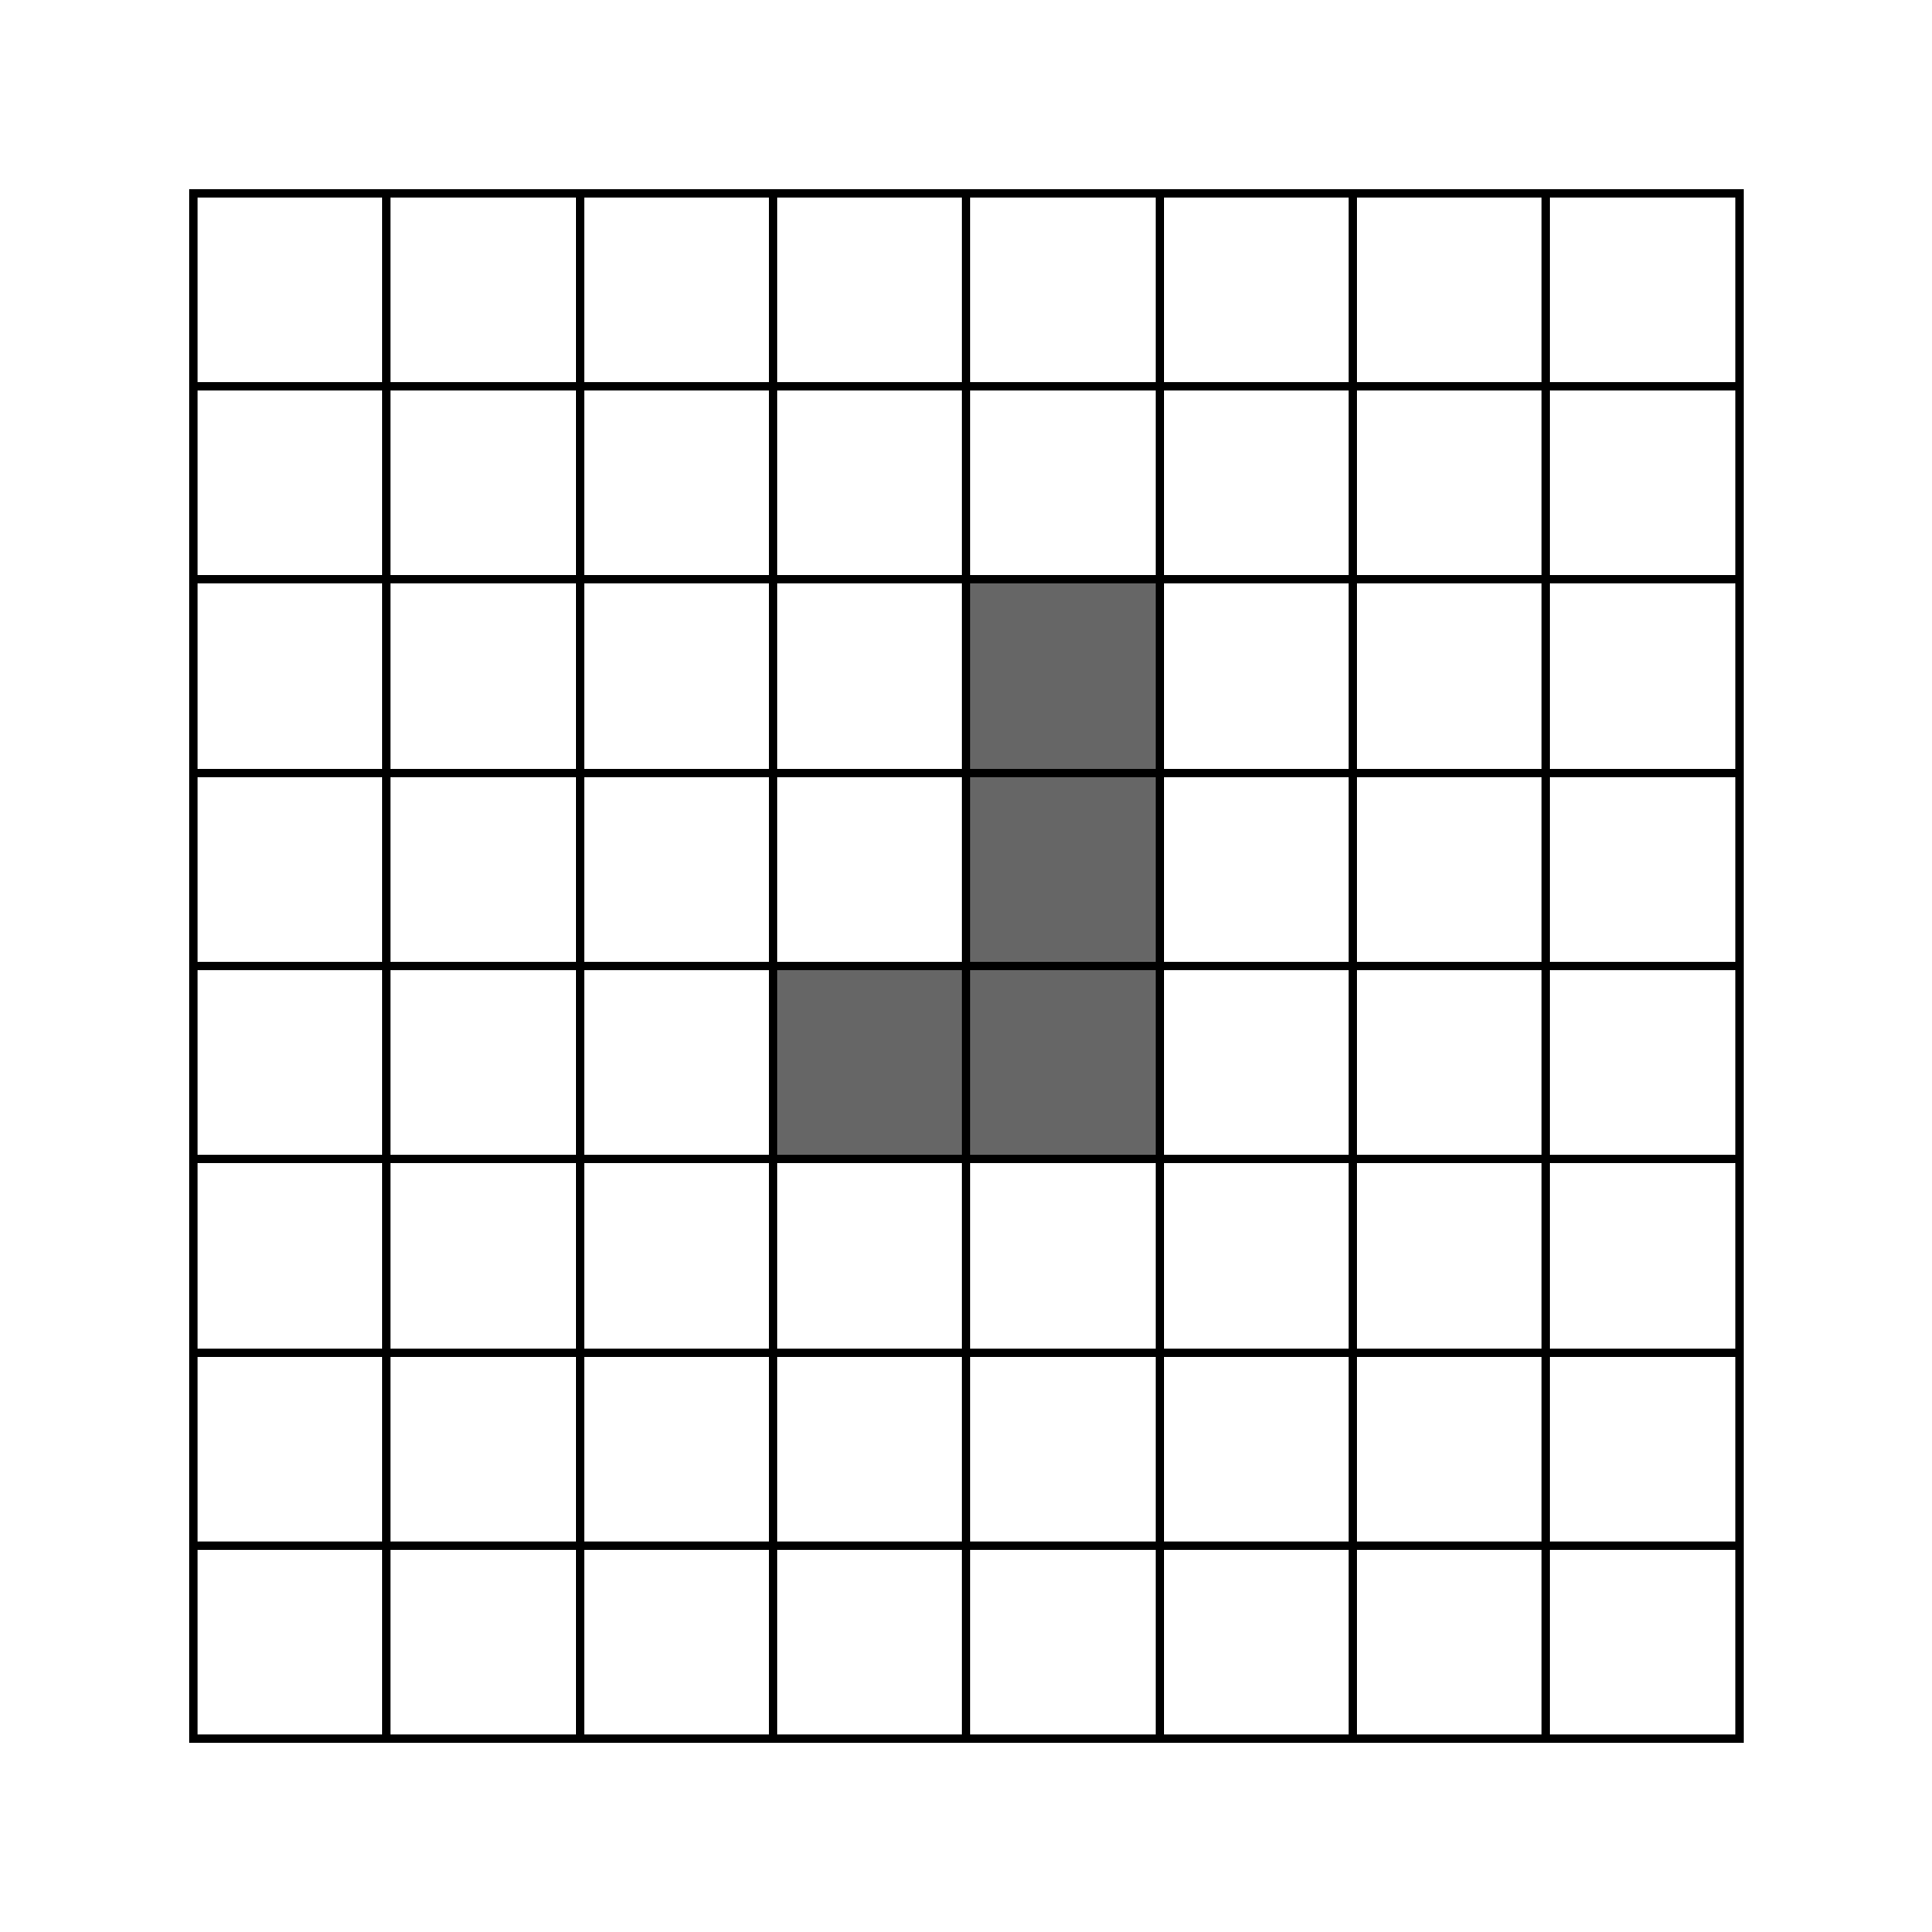
\includegraphics[width=0.2\textwidth]{chapters/cellularautomaton_images/Life1}
	\label{fig:ca_life_four_steps_step1}
}
\subfigure[Step 2]{
	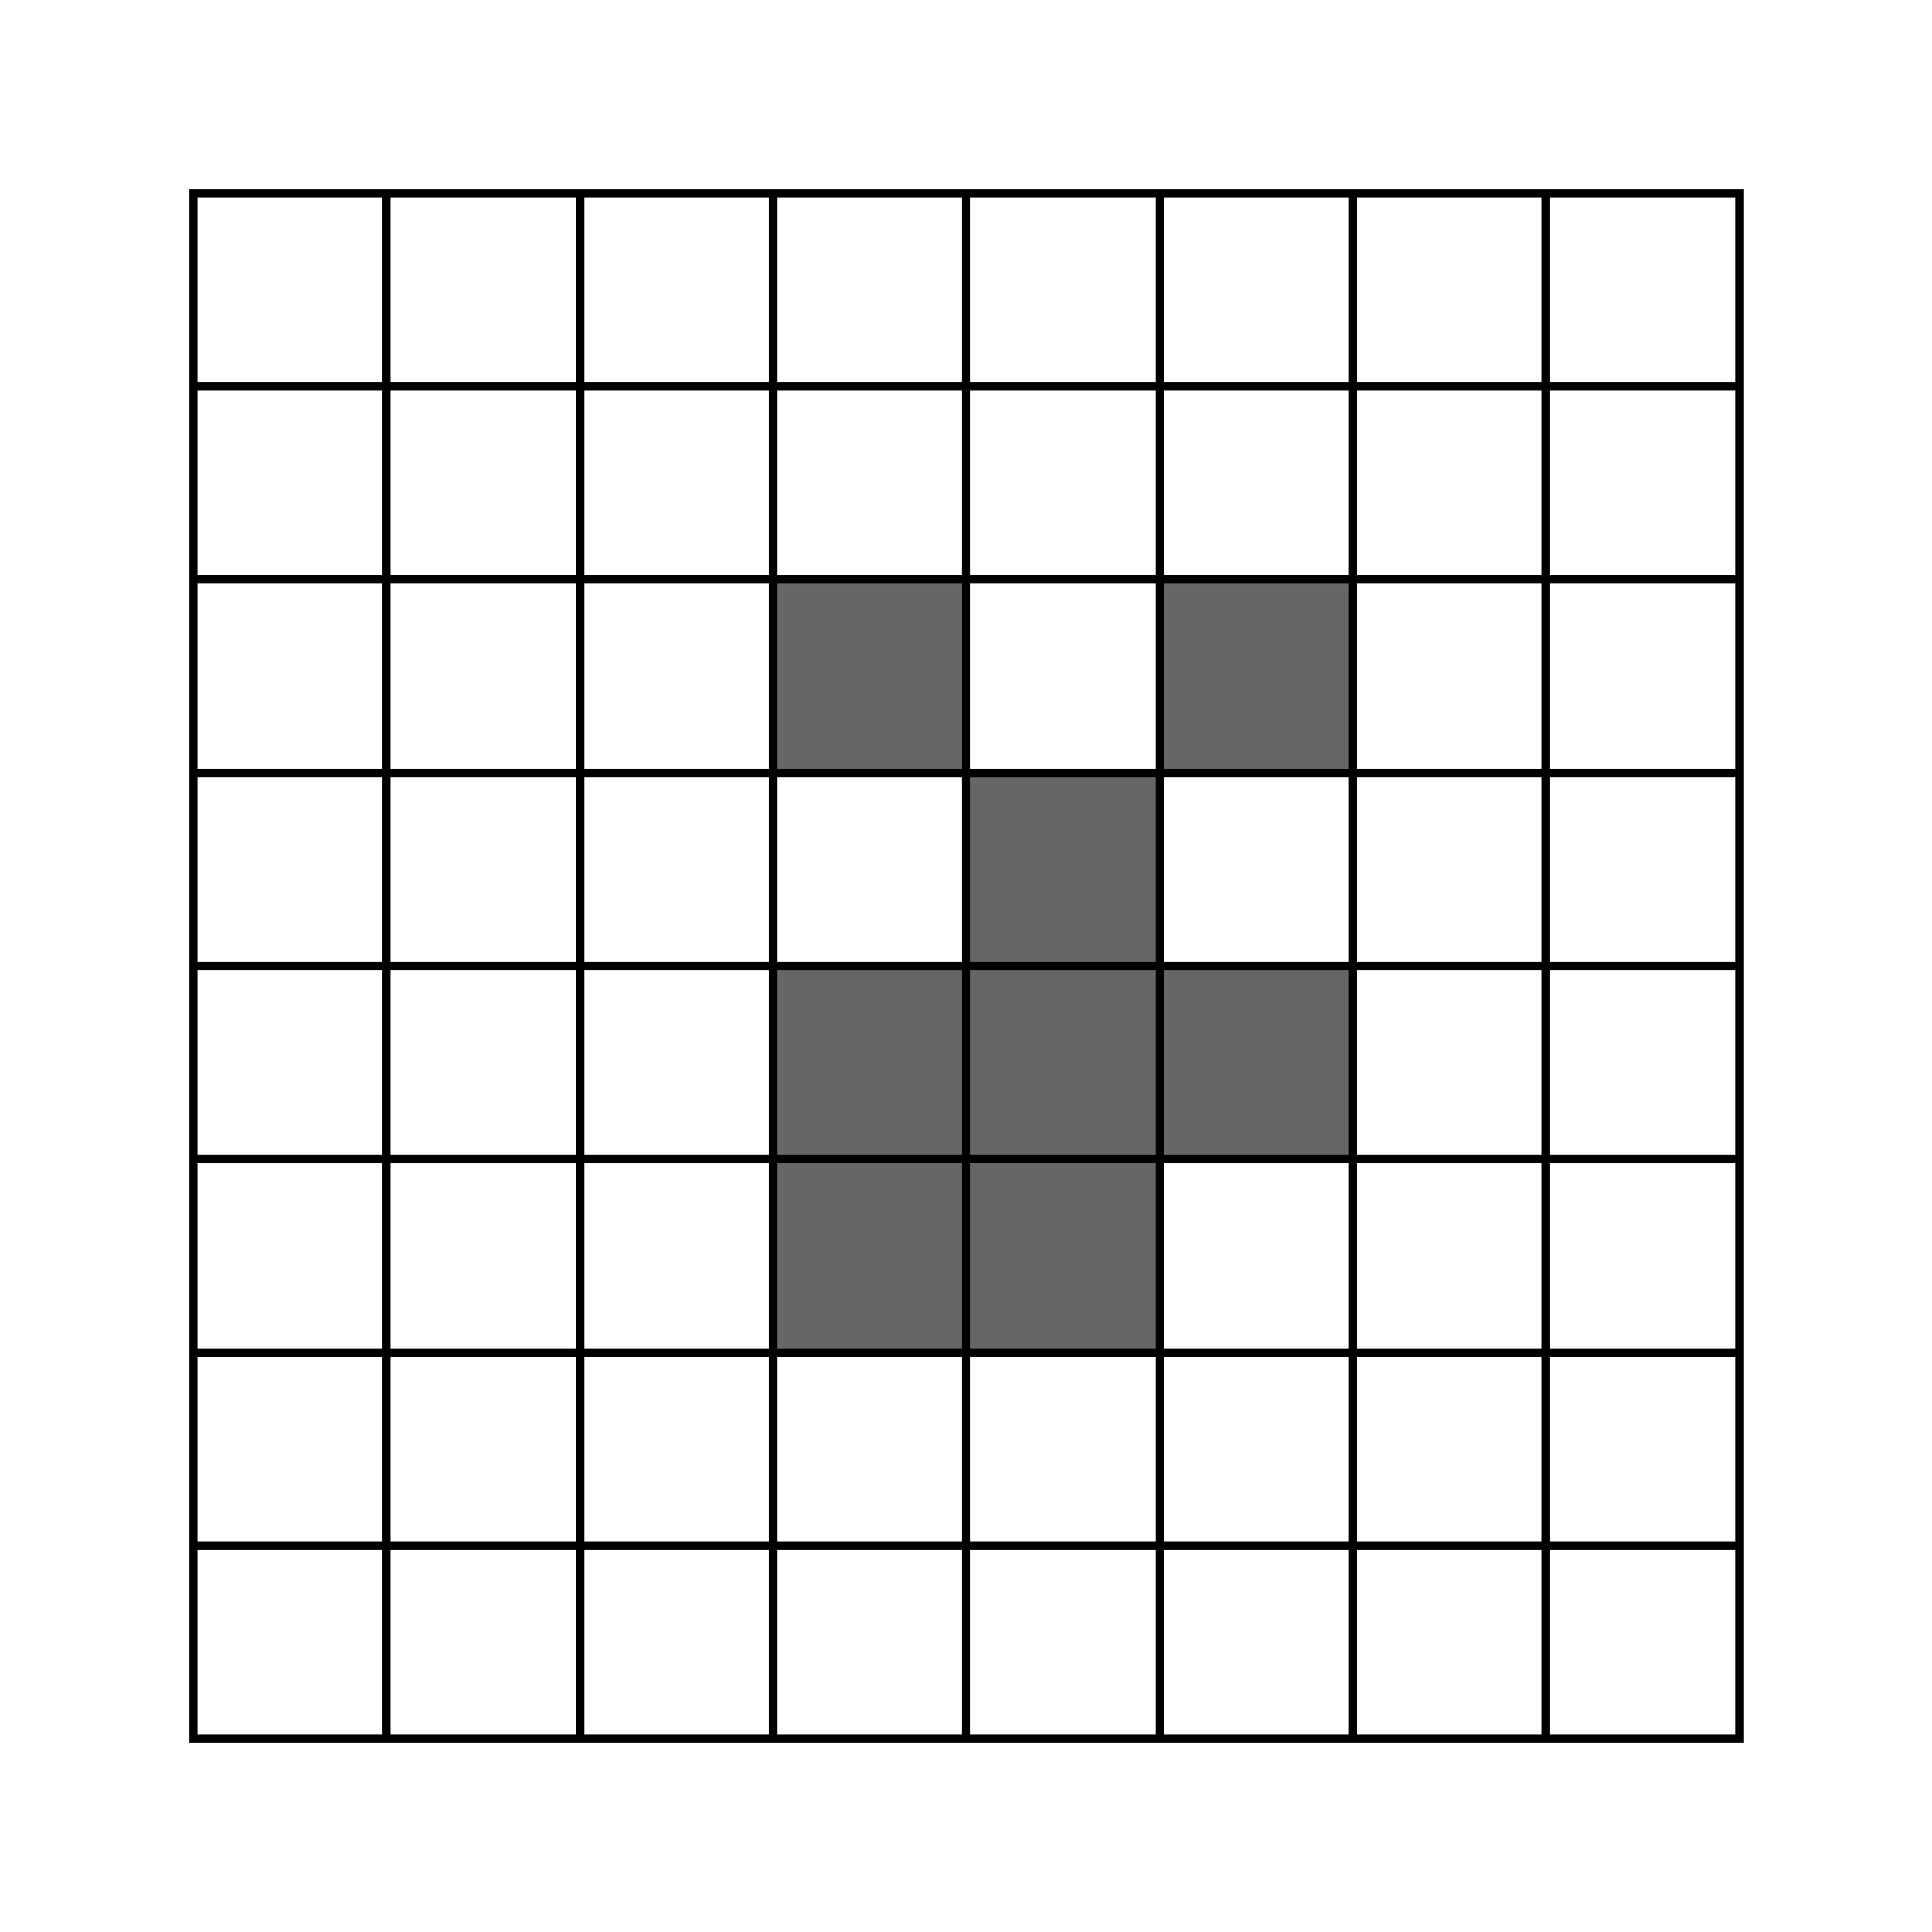
\includegraphics[width=0.2\textwidth]{chapters/cellularautomaton_images/Life2}
	\label{fig:ca_life_four_steps_step2}
}
\subfigure[Step 3]{
	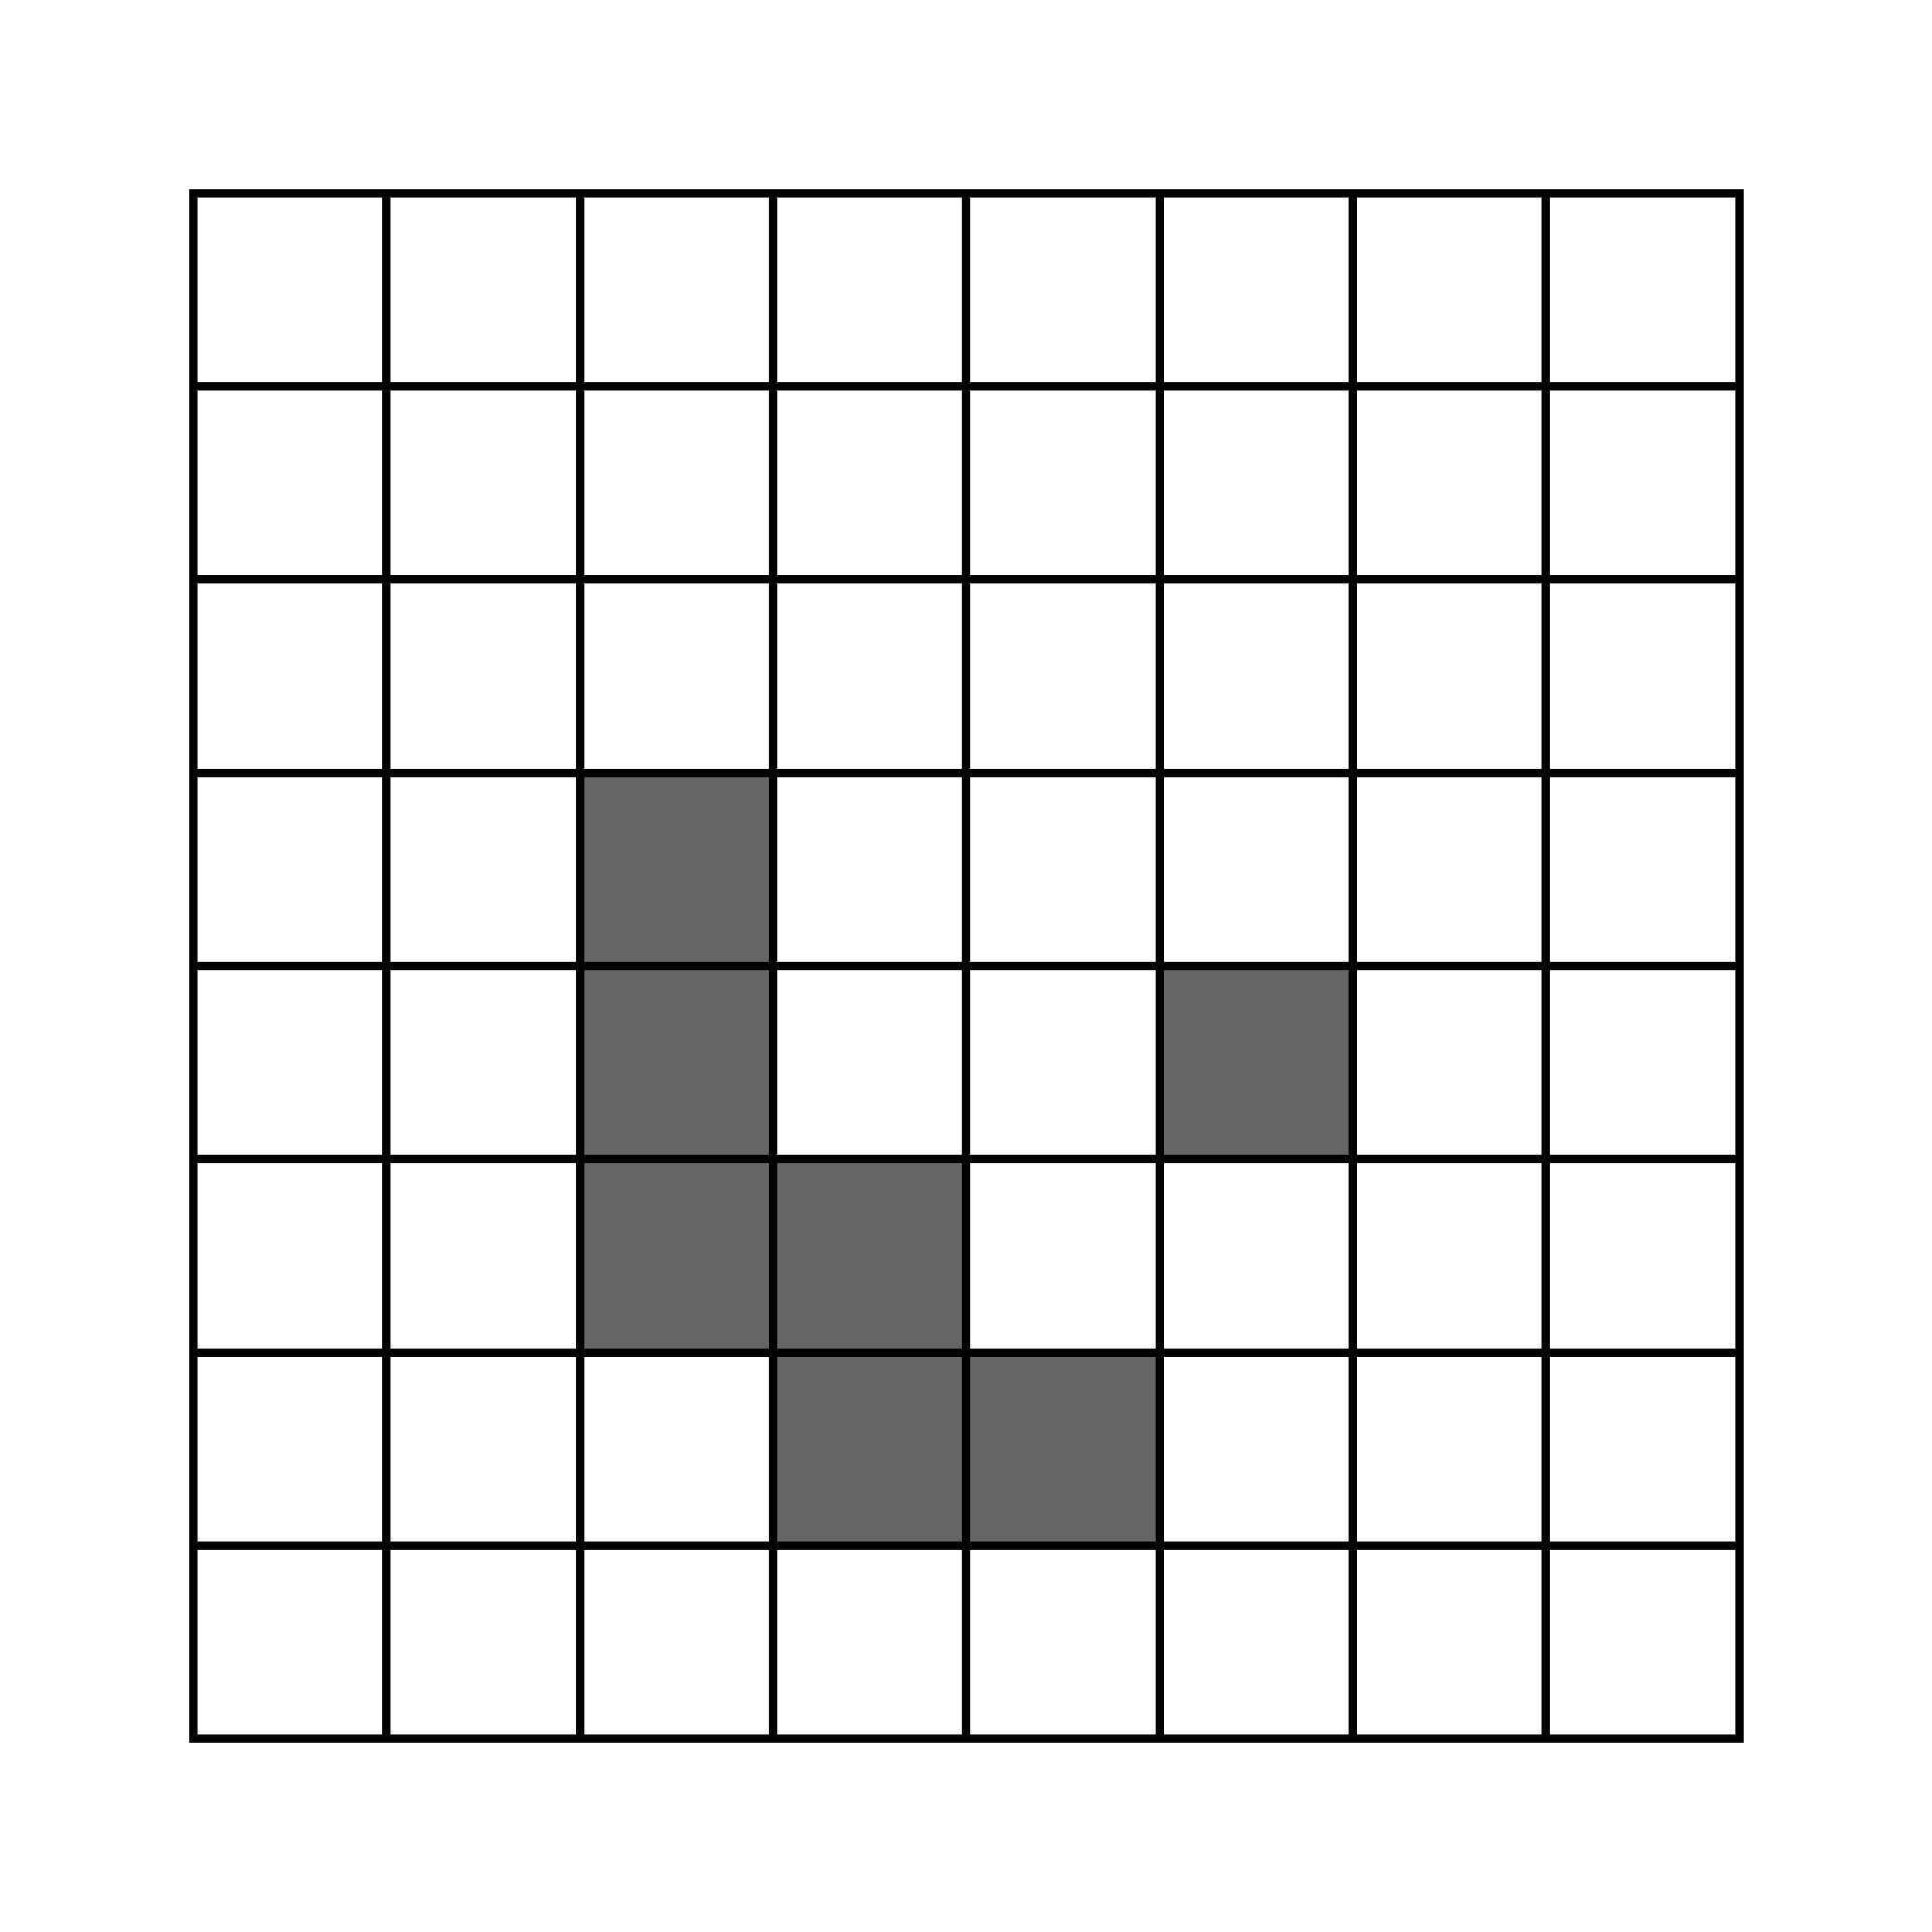
\includegraphics[width=0.2\textwidth]{chapters/cellularautomaton_images/Life3}
	\label{fig:ca_life_four_steps_step3}
}
\subfigure[Step 4]{
	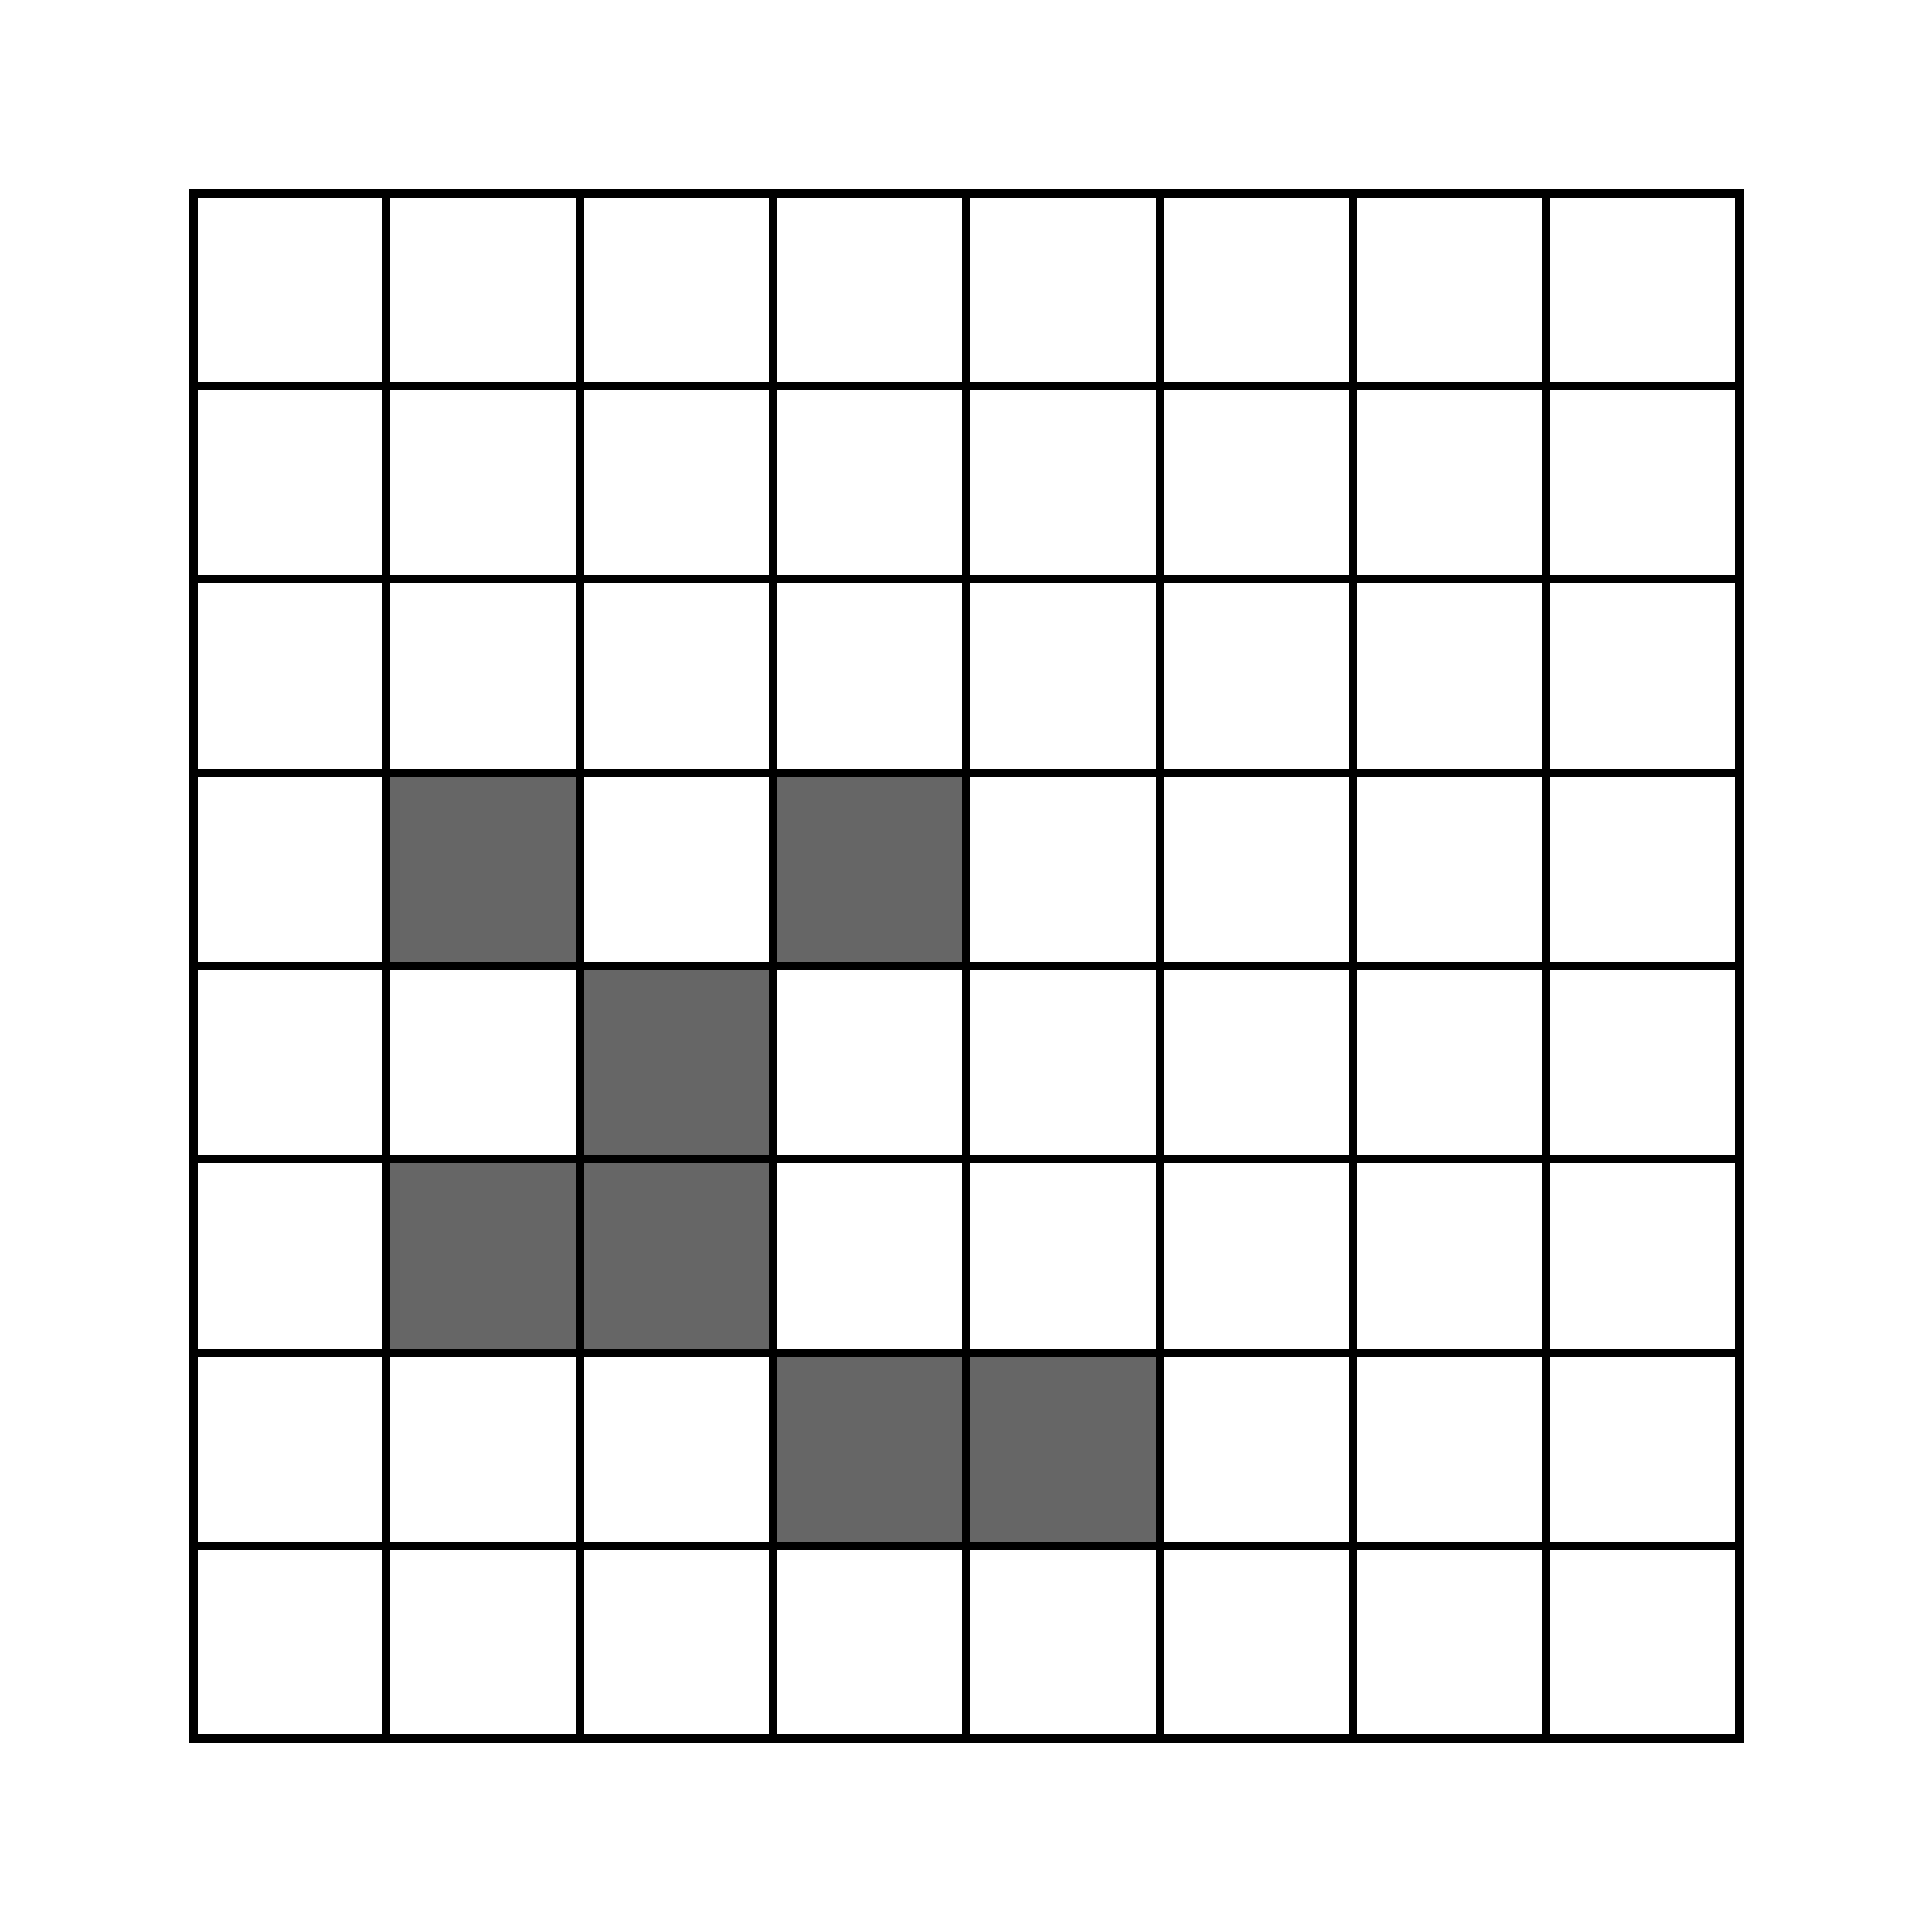
\includegraphics[width=0.2\textwidth]{chapters/cellularautomaton_images/Life4}
	\label{fig:ca_life_four_steps_step4}
}
\caption[Example of state evolution in \emph{Conway's Game of Life}]{\label{fig:ca_life_four_steps}The first four states of a \ac{CA} following the rules of \emph{Conway's Game of Life}. Grey squares represent live cells, white squares represent dead cells. The initial pattern in \subref{fig:ca_life_four_steps_step1} produces increasingly complex states, e.g. \subref{fig:ca_life_four_steps_step2} to \subref{fig:ca_life_four_steps_step4}, as the system evolves according to a few simple rules. The state of a cell depends only on the states of its immediate neighbours in the preceding step, allowing the state to be computed in parallel, using only local information.}
\end{figure}

%% --------------------------------------------------
%% SECTION: Cellular Automata & Track Finding
%% --------------------------------------------------
\section{Cellular Automata \& Track Finding}\label{sec:cellularautomaton_history}
The use of a \ac{CA} for tracking in high-energy physics was proposed in \citep{Glazov1992} for filtering tracks in \ac{MWPC} detectors. They define a cluster of continuous hits to be a living cell and an empty region to be a dead cell. In order to support interrupted tracks due to detector inefficiencies, they also propose phantom cells, which may also be either living or dead, giving their \ac{CA} four states.

Neighbours are determined by the range of admissible angles at which a track may run through the cluster of hits corresponding to any given cell. The update rules create phantoms if there are living neighbours on either side which are compatible with the track model, and destroy cells if there are too few ($< 2$) or too many ($> 4$) neighbours. The first part is designed to cope with gaps in a track due to detector inefficiencies, while the last part filters out noise hits. The \ac{CA} is iterated until a stable configuration is reached, at which point the remaining real live cells correspond to the hits of filtered tracks. A similar procedure is also proposed in \citep{Casolino1995}.

An important development was made in \citep{Kisel1997} where it was proposed to make a \ac{CA} in which the cells were straight line segments linking hits or clusters in adjacent layers of a detector (or skipping at most one layer, to account for detector inefficiencies). The neighbours of a cell are considered to be those cells which share a hit or cluster at one end and have some angle $\phi < \phi_\mathrm{max}$ between the line segments.

An integer number is assigned as the state of each cell, associated with the cell's position along the track. Initially, all cells get the state 1 and at each step of evolution the update rule looks at neighbours in preceding layers and increases the position value by 1 if there is a neighbouring cell with the same state. Evolution stops when no neighbouring cells have the same state. As usual, time evolves in discrete steps with cell updates occurring simultaneously.

After this \ac{CA} is run the final state gives the positions of all segments of all track candidates. The track candidates are formed by starting with the highest valued segments and adding the neighbour with the previous position value, all the way back to position value 1. This approach not only filters out noise but also \emph{clusters} the track candidates into distinct clusters.

A further example of the use of line segments for the cells of a \ac{CA} with similar update rules, considering neighbours to be leftward segments sharing a common space point and having some angle no greater than a maximum \emph{breaking angle} between adjacent segments is considered for the HERA-B vertex detector in \citep{Abt2002}. The approach is extended to 3D tracks in a layered scintillator bar detector with horizontal and vertical layers in \citep{Maesaka2005}, where the \ac{CA} is run in 2D over the $xz$-plane and the $yz$-plane independently, and tracks are combined into a three-dimensional reconstruction using $z$ positions and timing information.

%% --------------------------------------------------
%% SECTION: 3D Cellular Automaton for Track Finding
%% --------------------------------------------------
\section{A 3D Cellular Automaton for Track Finding}\label{sec:cellularautomaton_algorithm}
The \ac{CARLA} algorithm is composed of several procedures, each of which is described in detail. The algorithm runs through each of the following stages in turn:

\begin{enumerate}
	\item Preprocessing
	\item Cell generation
	\item Forward run
	\item Reverse run
	\item Postprocessing
\end{enumerate}

The pre- and post-processing stages are specific to the form of data used; preprocessing typically includes a charge weighting process followed by a re-scaling to reduce the number of input hits, while postprocessing typically involves merging track segments and filtering out short fragments. In the following algorithm descriptions, the term \emph{leftward} means having lower coordinate value along the beam axis, which is defined to be the $x$-axis in the simulation. Similarly, \emph{rightward} means having higher coordinate value along the beam axis.

%% --------------------------------------------------
%% SUBSECTION: Preprocessing
%% --------------------------------------------------
\subsection{Terminology}
The following description of the cellular automaton reconstruction algorithm makes extensive use of the terms \emph{forward}, \emph{backward}, \emph{left} and \emph{right}. For the most part, these terms originated in the papers describing earlier implementations of cellular automata for tracking, described earlier in this chapter. Precise definitions in the context of the algorithm used here are given below. Note that the algorithm presented is, to the maximum extent possible, fully three-dimensionally aware and that, in particular, the concept of left or right is relative, even though it is required in order to avoid ambiguity about how to proceed in any given step. The algorithm cannot be described without defining the terms, but the terms cannot be properly defined without describing the algorithm; the definitions here should be taken together with the complete description that follows.

\vspace{1em}\hrule\vspace{1em}
\begin{description}
    \item[Forward]
        The \emph{forward} run is the process by which the cellular automaton gives each cell a weight value, updating it until a stable state is reached (i.e. no weights change from one pass to the next). This process occurs across the entire 3D space, and may even be performed in parallel.
    
    \item[Reverse, or Backward]
        The \emph{reverse} run is the process by which the cellular automaton follows a chain of cells whose weights decrease from an arbitrary integer to $1$, descending by $1$ weight unit at a time. This process can occur in any direction in 3D space; the \emph{reverse} part relates to traversing a chain of cells from a high number to a low number.

    \item[Left and Right]
        The term \emph{left}, or \emph{leftward}, describes the relative position of one hit or cell when compared with another hit or cell. The positions are taken relative to a single direction vector in 3D, which is usually chosen to be along one of the axes of the detector. A typical choice is for this vector to be along the beam, with \emph{left} upstream and \emph{right} downstream, but the algorithm does not require this to be the case. All that is required is a relative sense of direction, consistent across the entire detector, but applied locally when comparing nearby points or cells.
\end{description}
\vspace{1em}\hrule\vspace{1em}


%% --------------------------------------------------
%% SUBSECTION: Preprocessing
%% --------------------------------------------------
\subsection{Preprocessing}\label{sec:cellularautomaton_preprocessing}
\subsubsection{Charge Weighting}\label{sec:cellularautomaton_preprocessing_charge_weighting}
A charge weighted smoothing procedure is applied to the raw hits before further processing occurs. This procedure is described in section \ref{sec:cellularautomaton_charge_weighting}.

\subsubsection{Scaling}\label{sec:cellularautomaton_scaling}
The run time of the \ac{CA} depends strongly on the hit multiplicity (which in turn determines the cell multiplicity). In order to reduce the run time, a re-scaling from $1\mm$ to $3\mm$ voxels is implemented after the charge weighting procedure. This re-scaling groups together hits within the same $3\mm \times 3\mm \times 3\mm$ region and represents them as a single cluster at the charge-weighted centroid position of those hits (calculated as for the charge weighting, with equation \ref{eqn:charge_weighted_avg_position}), but now containing the accumulated charge of all the hits within it.

%% --------------------------------------------------
%% SUBSECTION: Cell Generation
%% --------------------------------------------------
\subsection{Cell Generation}\label{sec:cellularautomaton_cell_generation}
Cell generation is the process by which cells are made from pairs of hits. A cell consists of a leftward and rightward hit pair, and represents the line between the two hits, pointing from the leftward hit to the rightward hit.  In principle, each possible pairing of points within a fixed radius could produce a cell, but for speed and performance reasons it is better to build the cells more selectively. The algorithm below does this in a manner which produces the required cells with very little overhead.

For each hit in the event:
\begin{enumerate}
	\item Build a list of neighbouring hits within a $2\mm$ radius; in this implementation a \ac{KDTree} is used for this near-neighbour search.
	\item Filter the neighbour list to select only those neighbours which are \emph{upstream} with respect to the beam direction, i.e. select only leftward neighbours.
	\item Generate a cell for each remaining leftward neighbour, pointing from that hit to the current central hit (from left to right); see figure \ref{fig:cellularautomaton_cellgen_normal}.
	\item If no leftward hits were found, i.e. no cells were generated in the previous step, expand the search radius by $0.05\mm$ and repeat the procedure above until either a cell is generated or the maximum search radius of $5.0\mm$ is reached; see figure \ref{fig:cellularautomaton_cellgen_expand}.
    \item If multiple cells were generated, filter out longer copies of cells with the same slope, using a comparison tolerance of $0.10$ on the slope components.\footnote{The value $0.10$ is chosen geometrically. Consider a $3\times 3$ grid of unit cells; a line running maximally through the diagonal has slope $\alpha = \tan^{-1}(3/3) = 0.98$, while a line which just touches the top right cell has slope $\alpha = \tan^{-1}(2/3) = 0.78$, a difference of $0.20$. The discrete, voxellised nature of the detector means that it is very difficult to distinguish between two lines with slopes less than half of this value because they hit almost identical voxels, and charge weighting smooths out the small differences that do exist. A value of $0.10$ is therefore used as the comparison tolerance for slopes.} This step avoids making long cells which ``jump'' over several shorter cells, which could lead to multiple interleaved tracks in the final reconstruction; see figure \ref{fig:cellularautomaton_cellgen_filter}.
\end{enumerate}

\begin{figure}
\centering
\subfigure[Normal operation]{\label{fig:cellularautomaton_cellgen_normal}
	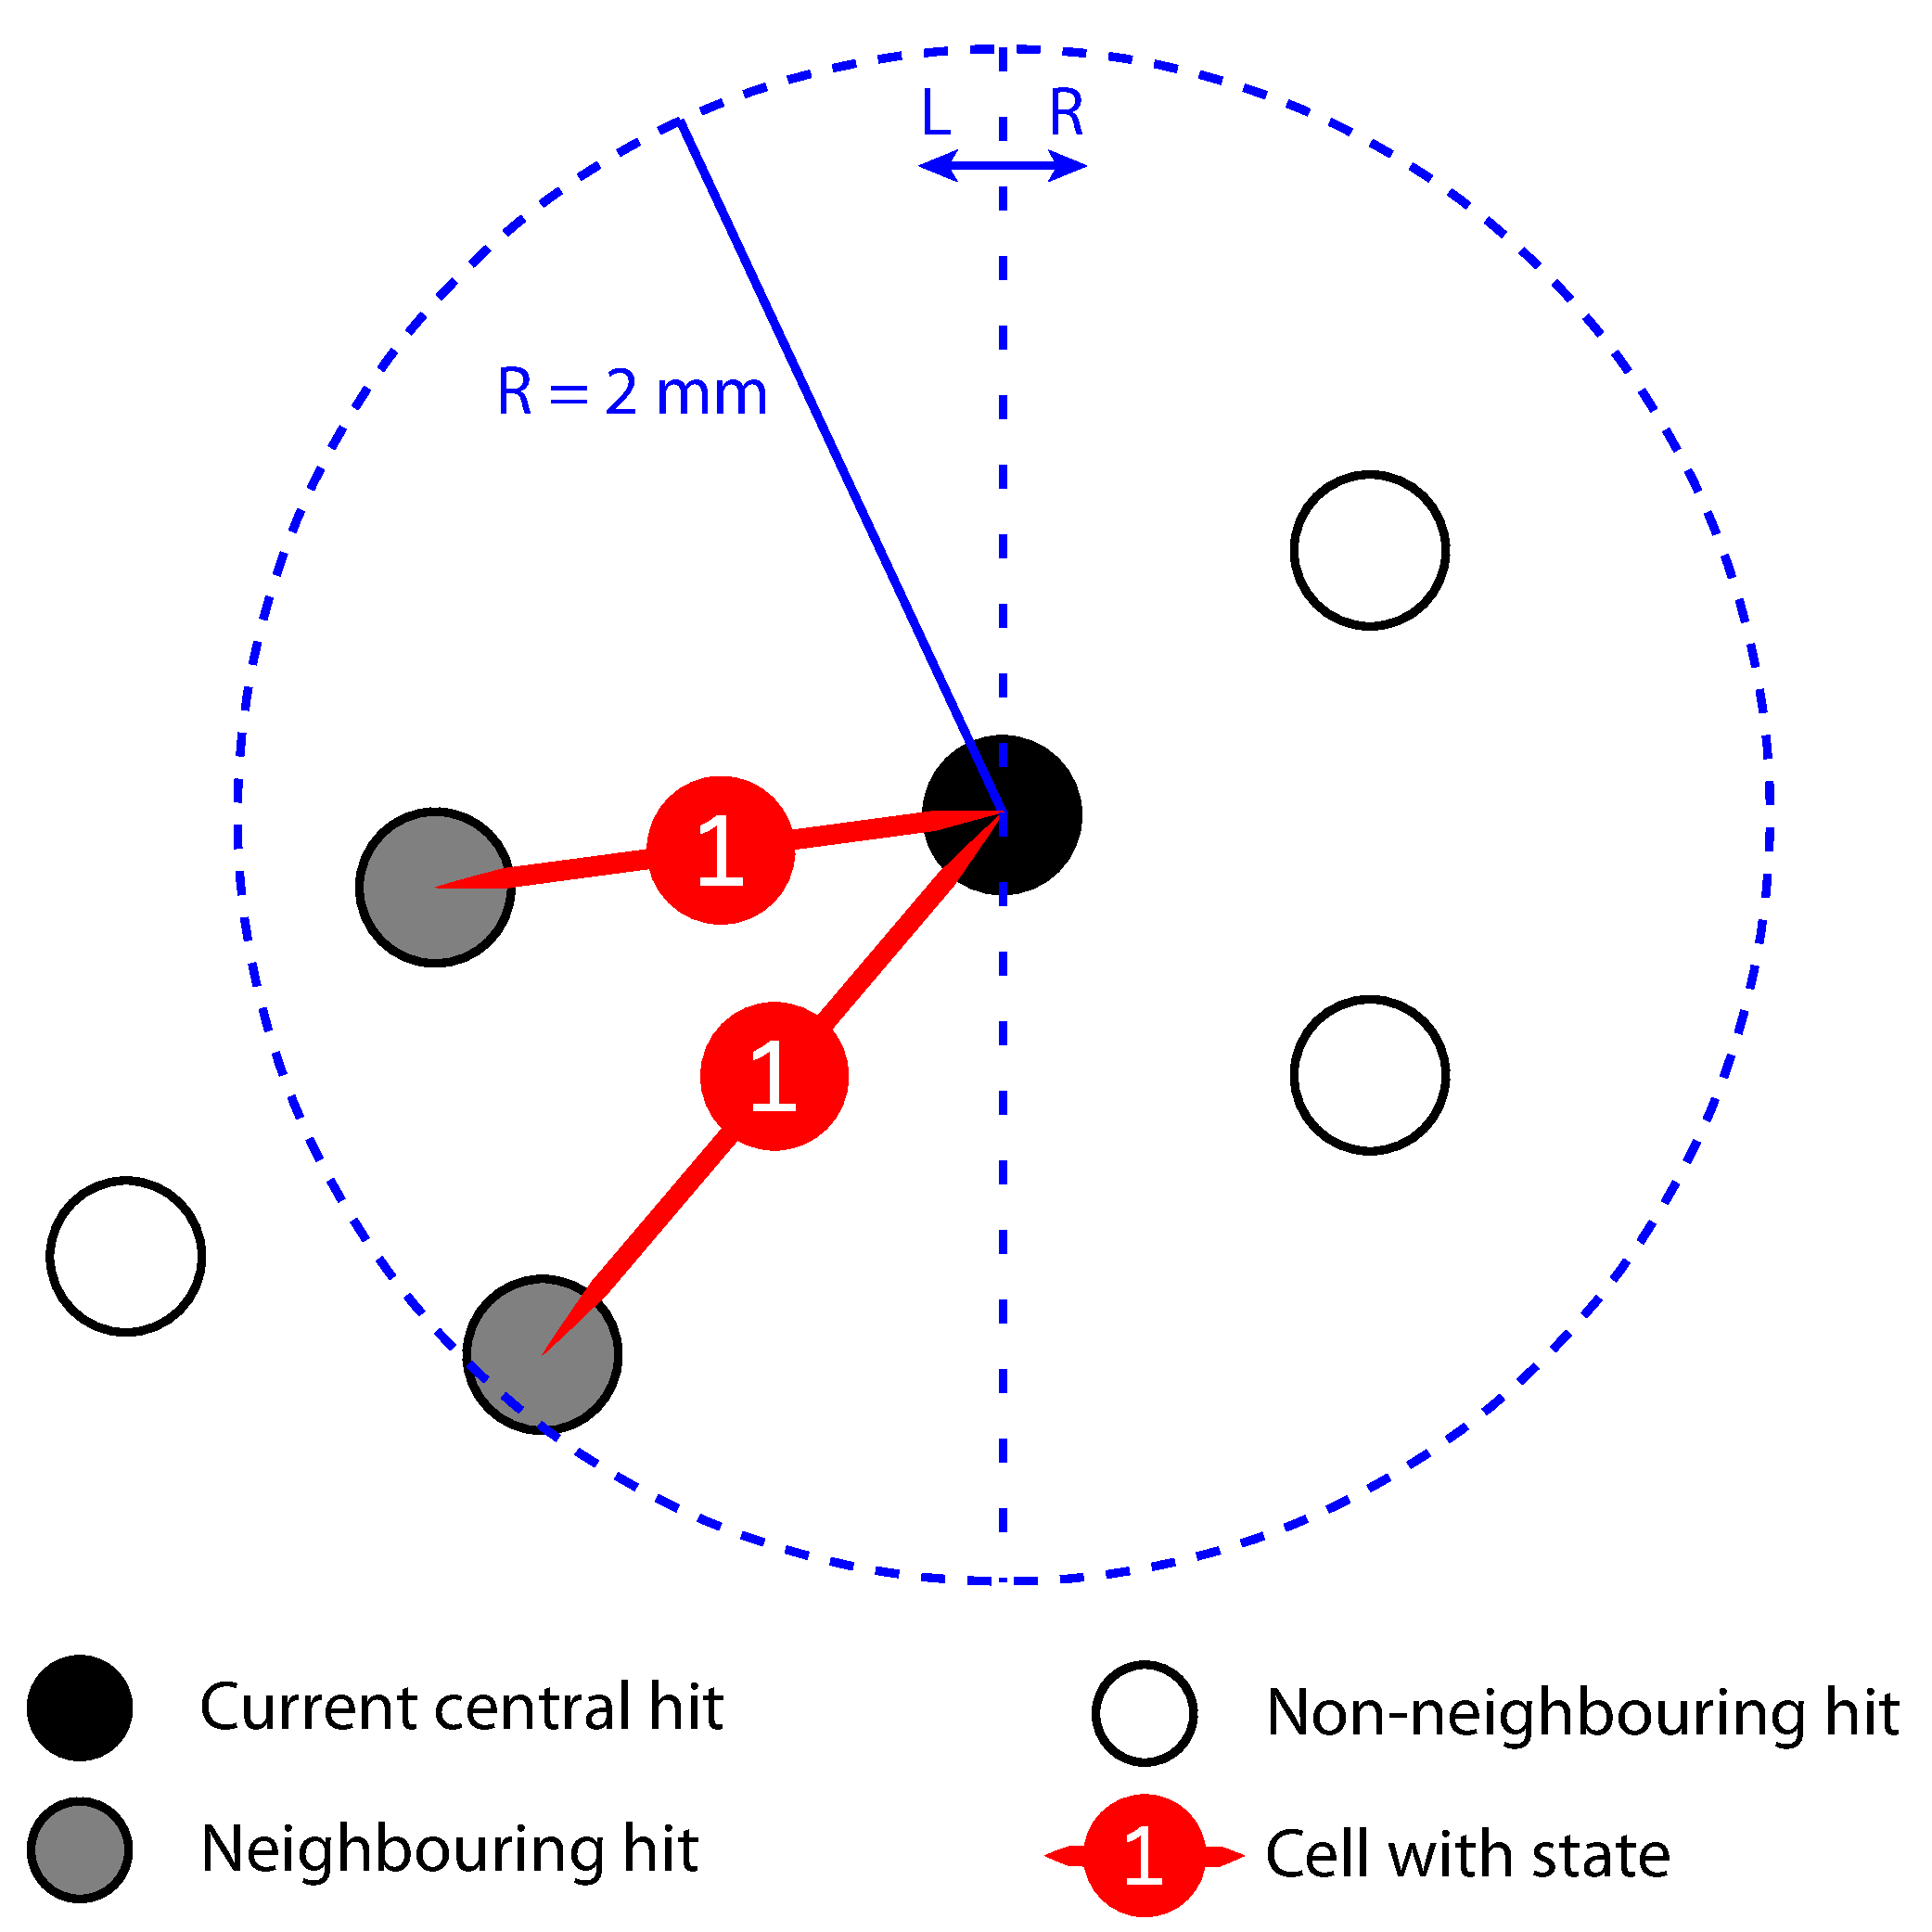
\includegraphics[width=0.3\textwidth]{chapters/cellularautomaton_images/CellGeneration1}
}
\subfigure[Expanding radius]{\label{fig:cellularautomaton_cellgen_expand}
	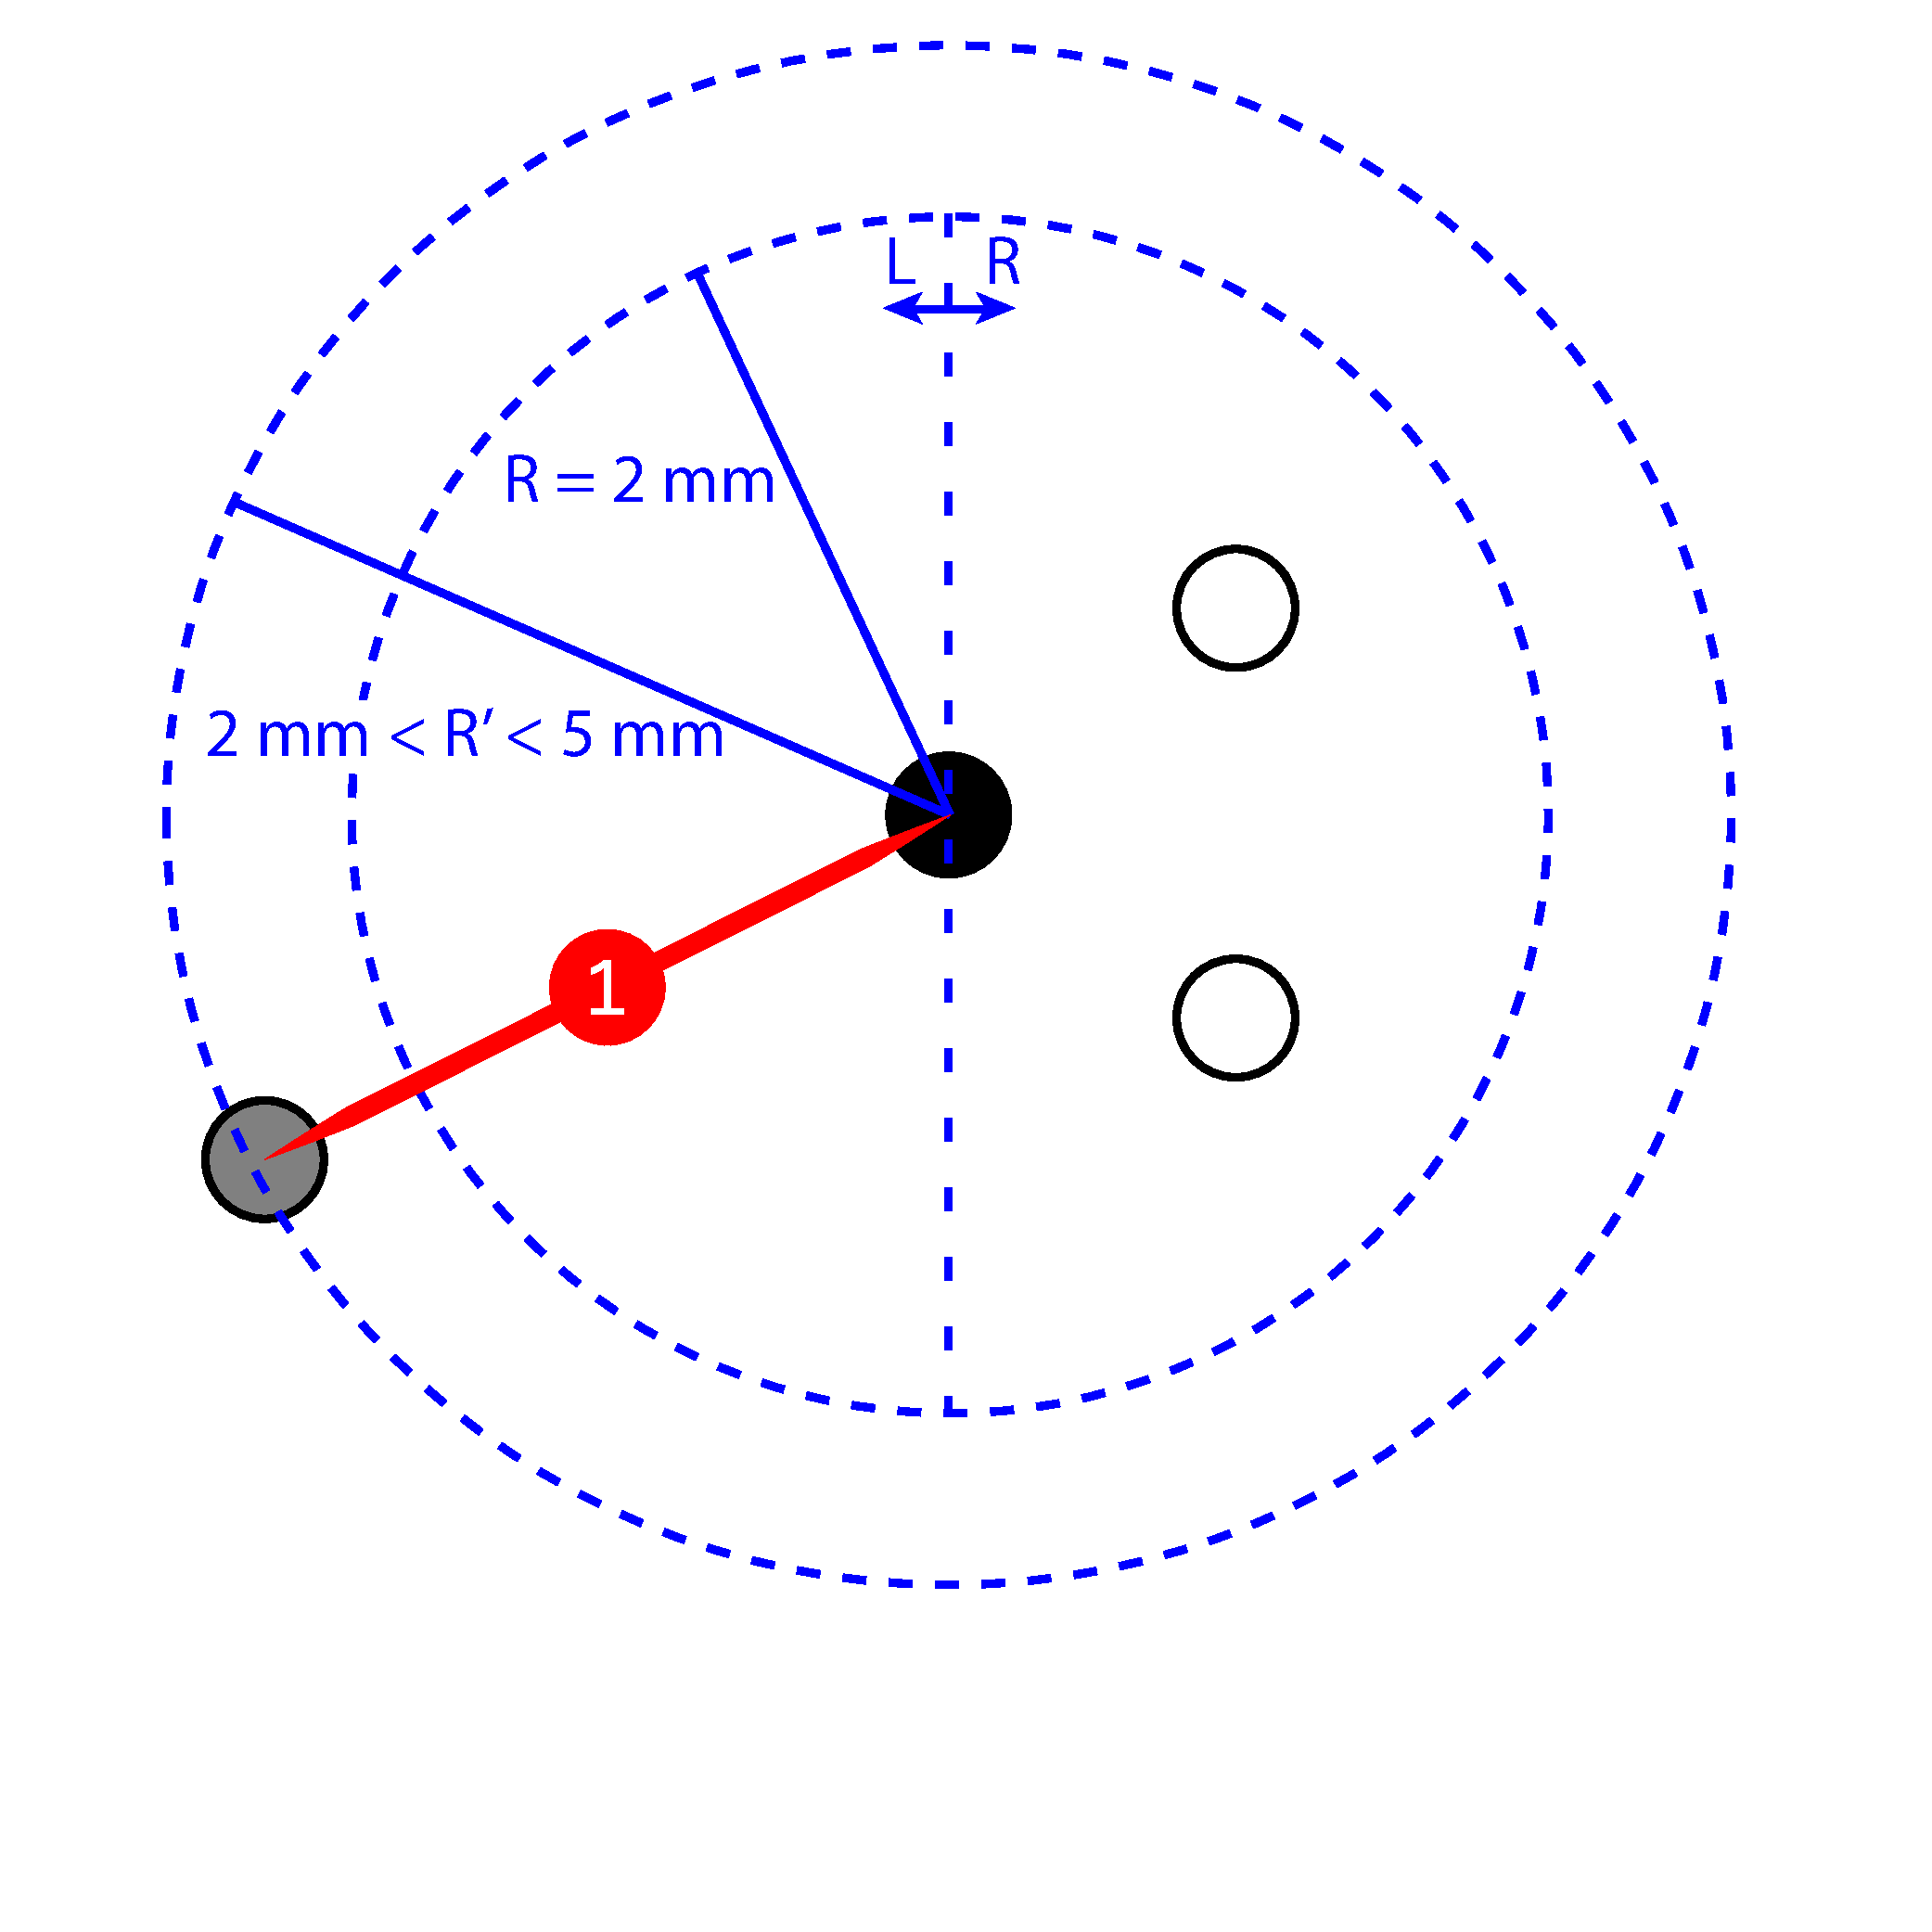
\includegraphics[width=0.3\textwidth]{chapters/cellularautomaton_images/CellGeneration2}
}
\subfigure[Filtering]{\label{fig:cellularautomaton_cellgen_filter}
	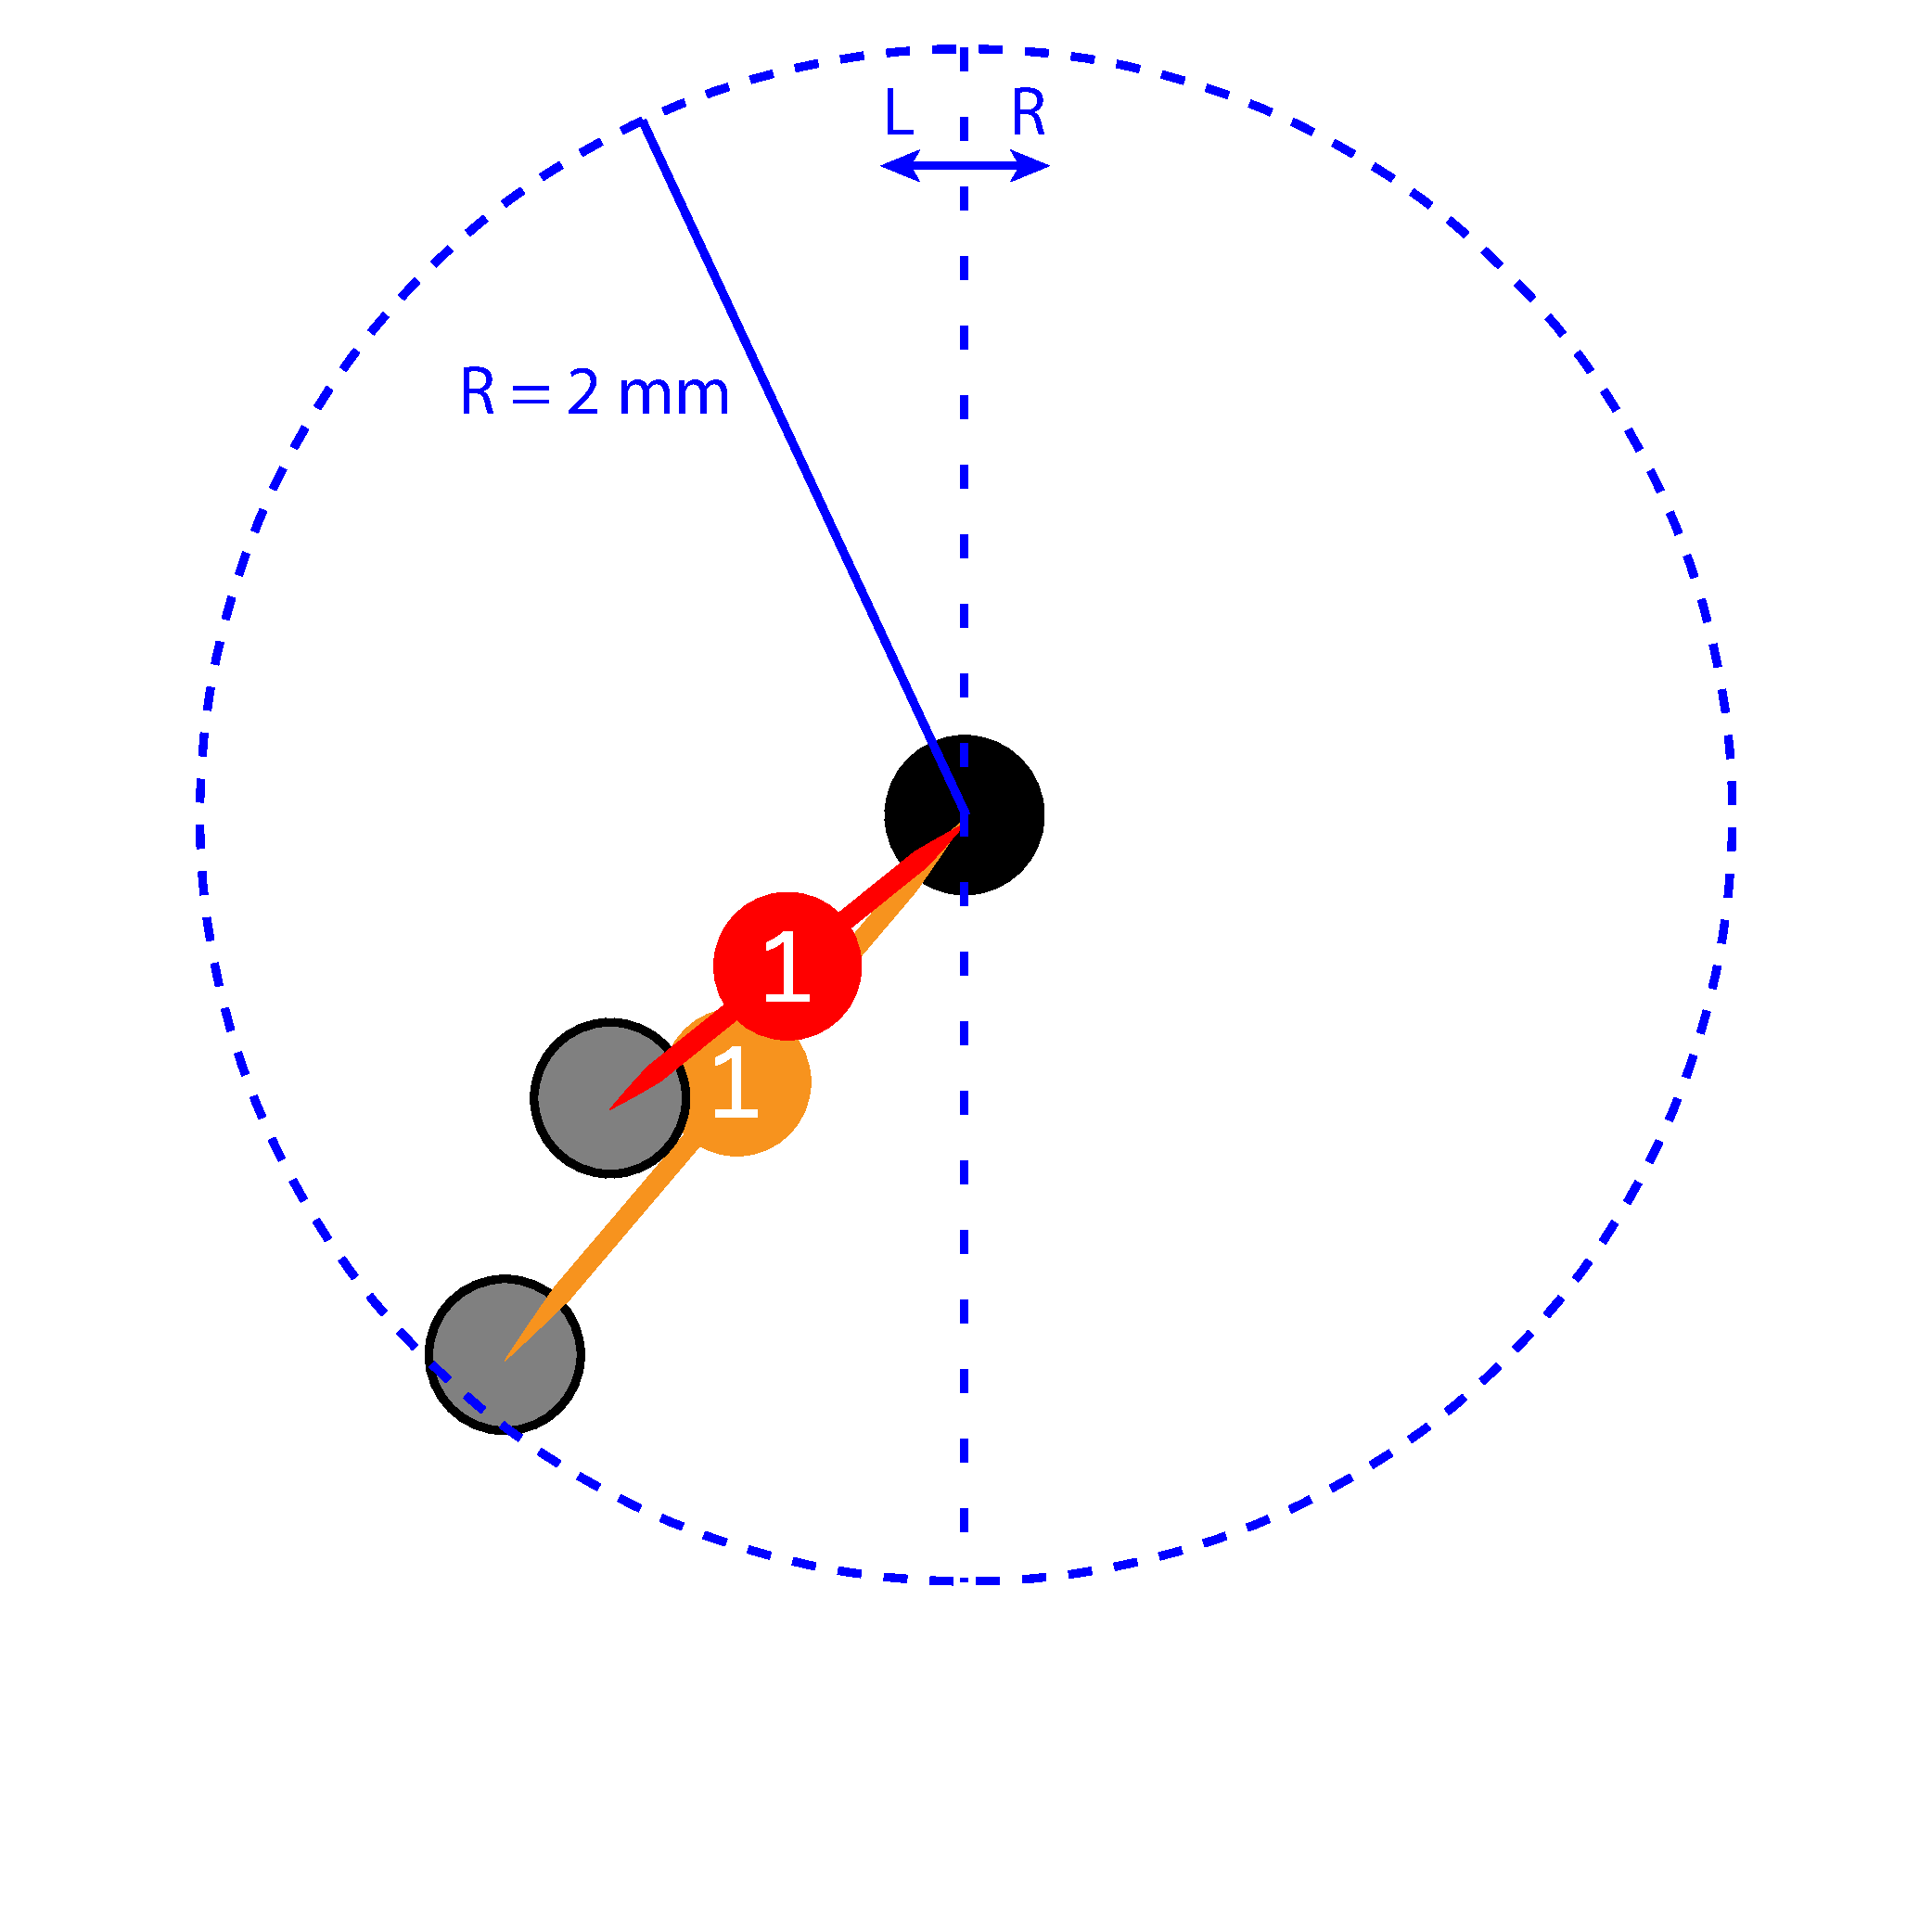
\includegraphics[width=0.3\textwidth]{chapters/cellularautomaton_images/CellGeneration3}
}
\caption[Illustration of the cell generation procedure in the CA algorithm]{\label{fig:cellularautomaton_cellgen}Illustration of the steps in the cell generation procedure for the \ac{CA}:\newline \subref{fig:cellularautomaton_cellgen_normal} creation of cells between a central point and any leftward neighbours within a $2\mm$ radius. \subref{fig:cellularautomaton_cellgen_expand} adaptive search radius expansion, which gradually expands the radius in $0.05\mm$ increments until either a leftward neighbour is found or a maximum radius of $5\mm$ is reached. \subref{fig:cellularautomaton_cellgen_filter} removal of cells if a shorter cell exists with similar slope; in this case, the red cell is retained while the longer orange cell is removed.}
\end{figure}

%% --------------------------------------------------
%% SUBSECTION: Forward Run
%% --------------------------------------------------
\subsection{Forward Run}\label{sec:cellularautomaton_forward_run}
The forward run is responsible for the evolution of the \ac{CA} from its initial state until a stable final state is reached. The forward step algorithm is run until the state remains unchanged, that is, until no cells needed to be updated in a step.

Before the first forward step, a mapping from cell to list of leftward neigbours is built. Cell A is a leftward neighbour of cell B if they share a central point (cell A's right point is identical to cell B's left point) and if the angle $\theta$ made between the two cell vectors is less than some threshold value $\theta_\mathrm{max}$. This mapping is used in every forward step, providing a speed boost over searching for leftward neighbours every time, since the number of cells does not change, and the cell properties are fixed (with the exception of cell state).

The forward step algorithm proceeds as follows (see also the illustration in figure \ref{fig:cellularautomaton_run}):
\begin{enumerate}
	\item For each cell with one or more leftward neighbours in the same state, mark the cell for update.
	\item Update all marked cells by increasing the value of their state by 1.
	\item Return the number of updated cells (if 0, this signals termination of the forward run).
\end{enumerate}

It is important not to update any cell state before all cells have been tested to see whether they must be updated. This prevents problems where a cell which would have been updated (because it had a neighbour with the same state) does not get updated because its neighbour was updated first. The forward step must appear to occur simultaneously across all cells; this opens up opportunities for parallelisation since each cell can be tested and marked for update independently. However, since this part of the algorithm is relatively quick for small numbers of cells, the current implementation does not do this in parallel.

\begin{figure}
\centering
\subfigure[Initial state]{\label{fig:cellularautomaton_run_initial}
	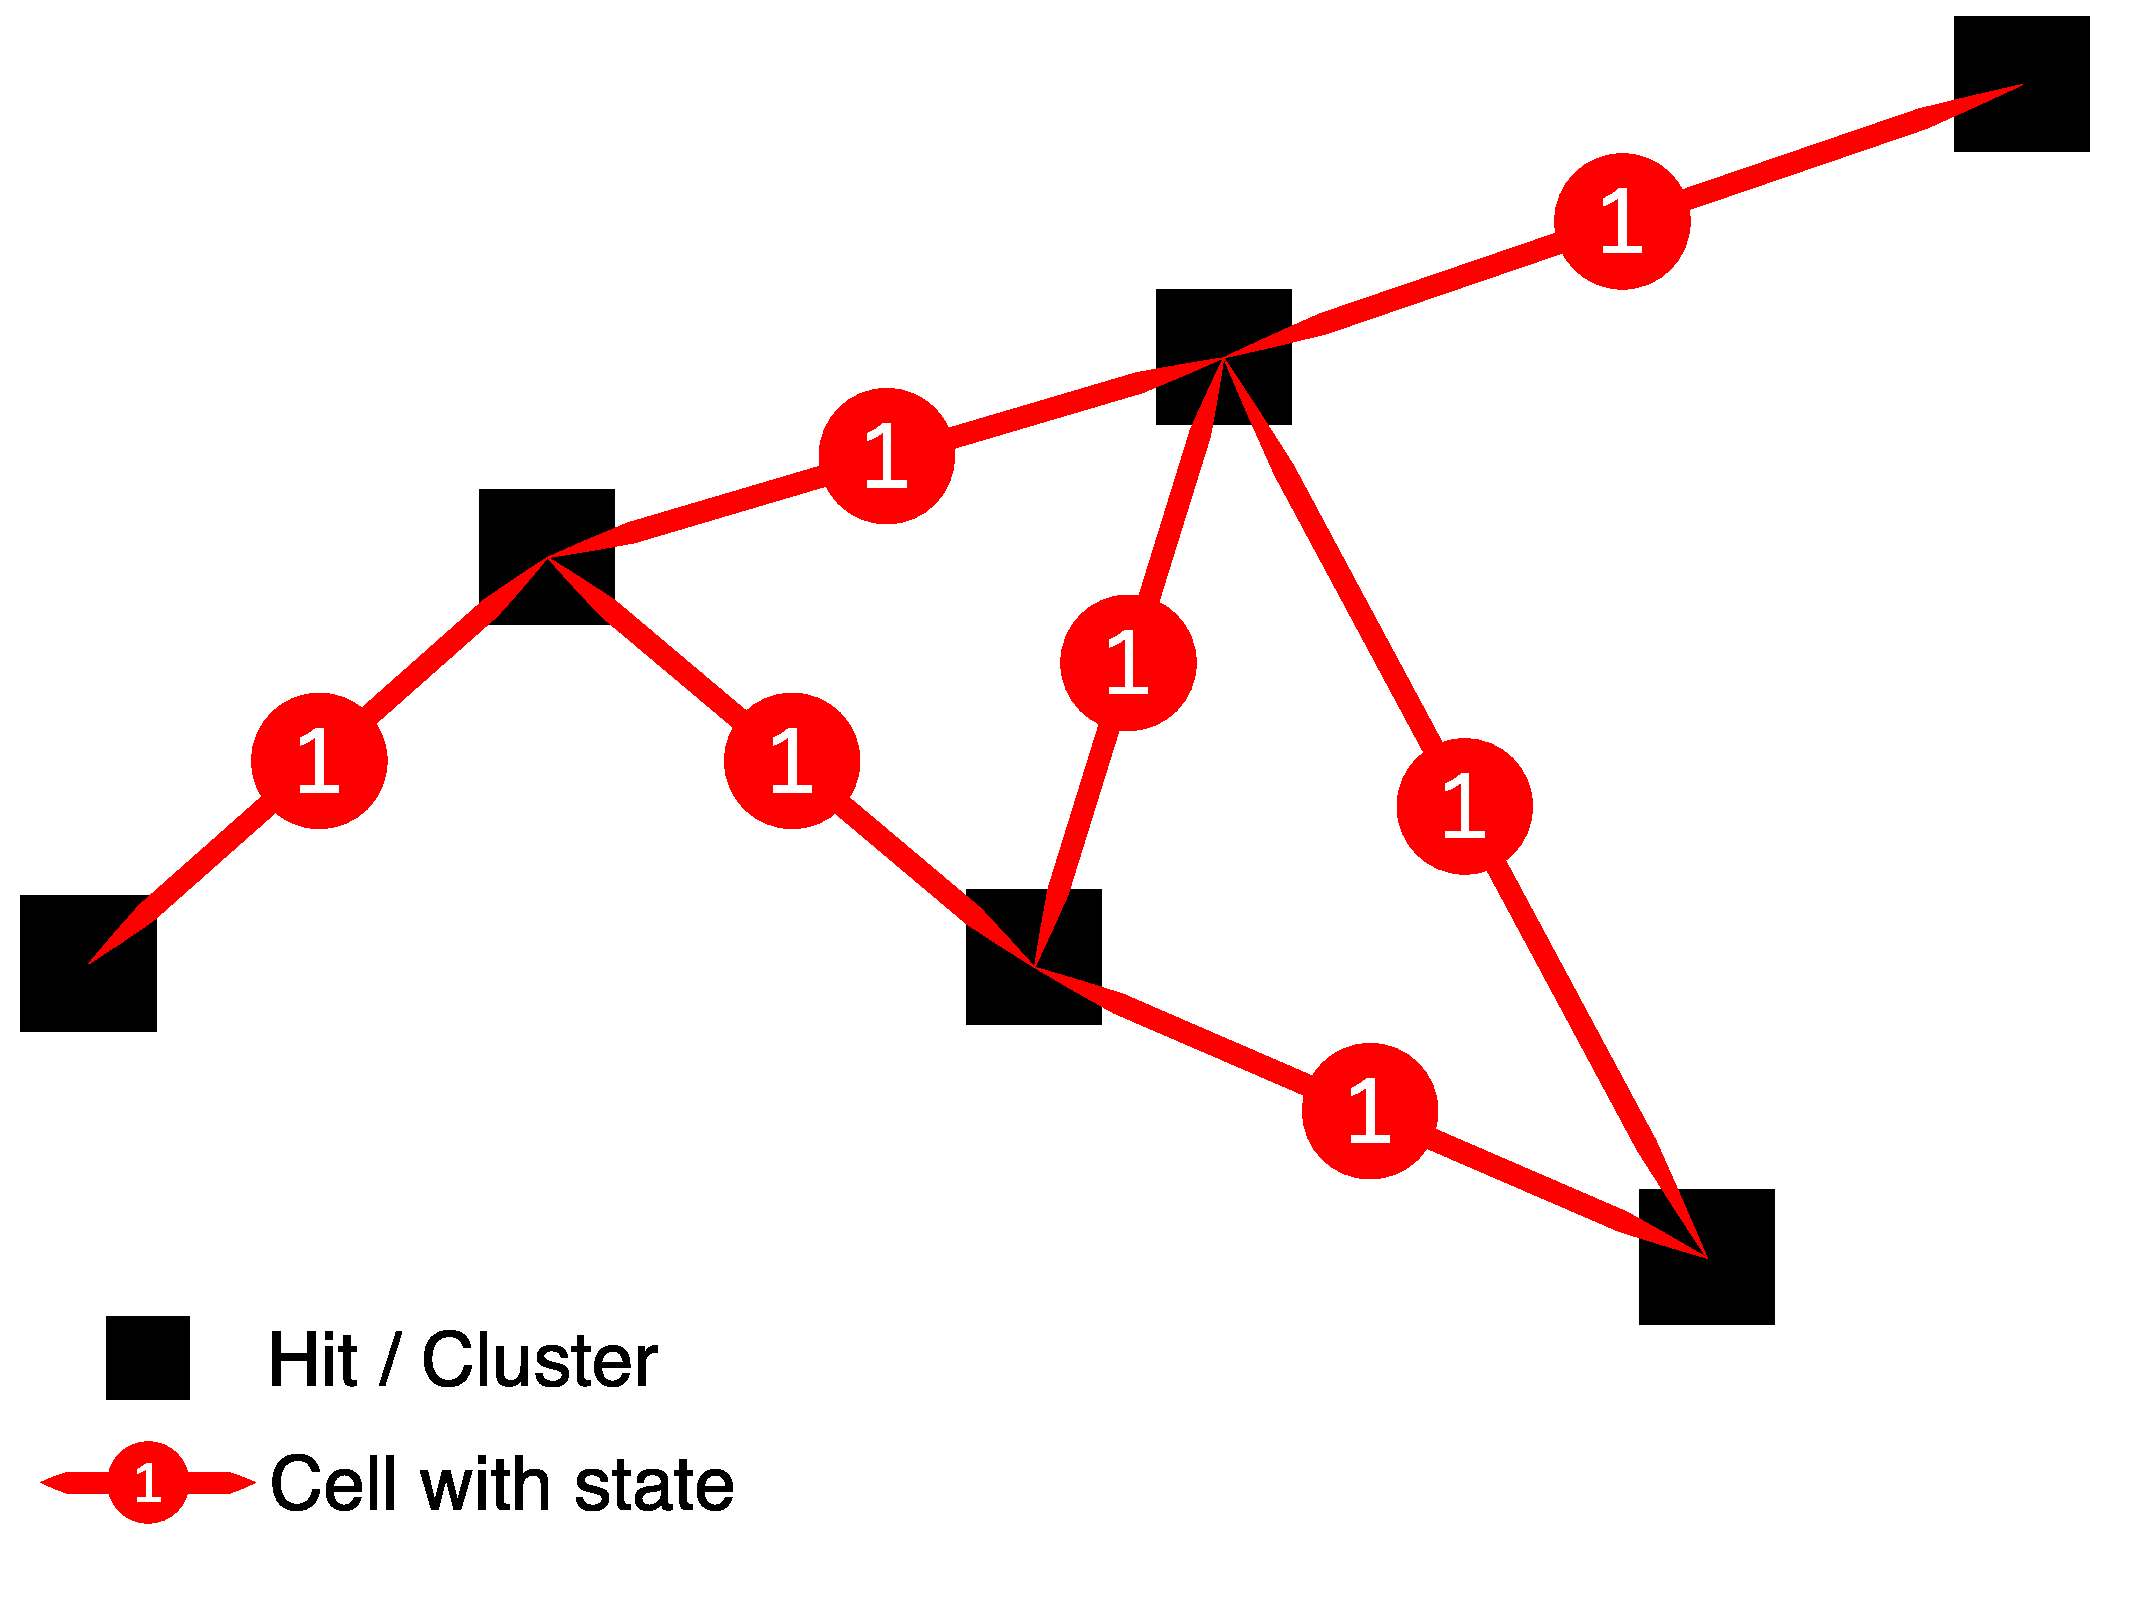
\includegraphics[width=0.3\textwidth]{chapters/cellularautomaton_images/ca-fig1}
}
\subfigure[Final state]{\label{fig:cellularautomaton_run_final}
	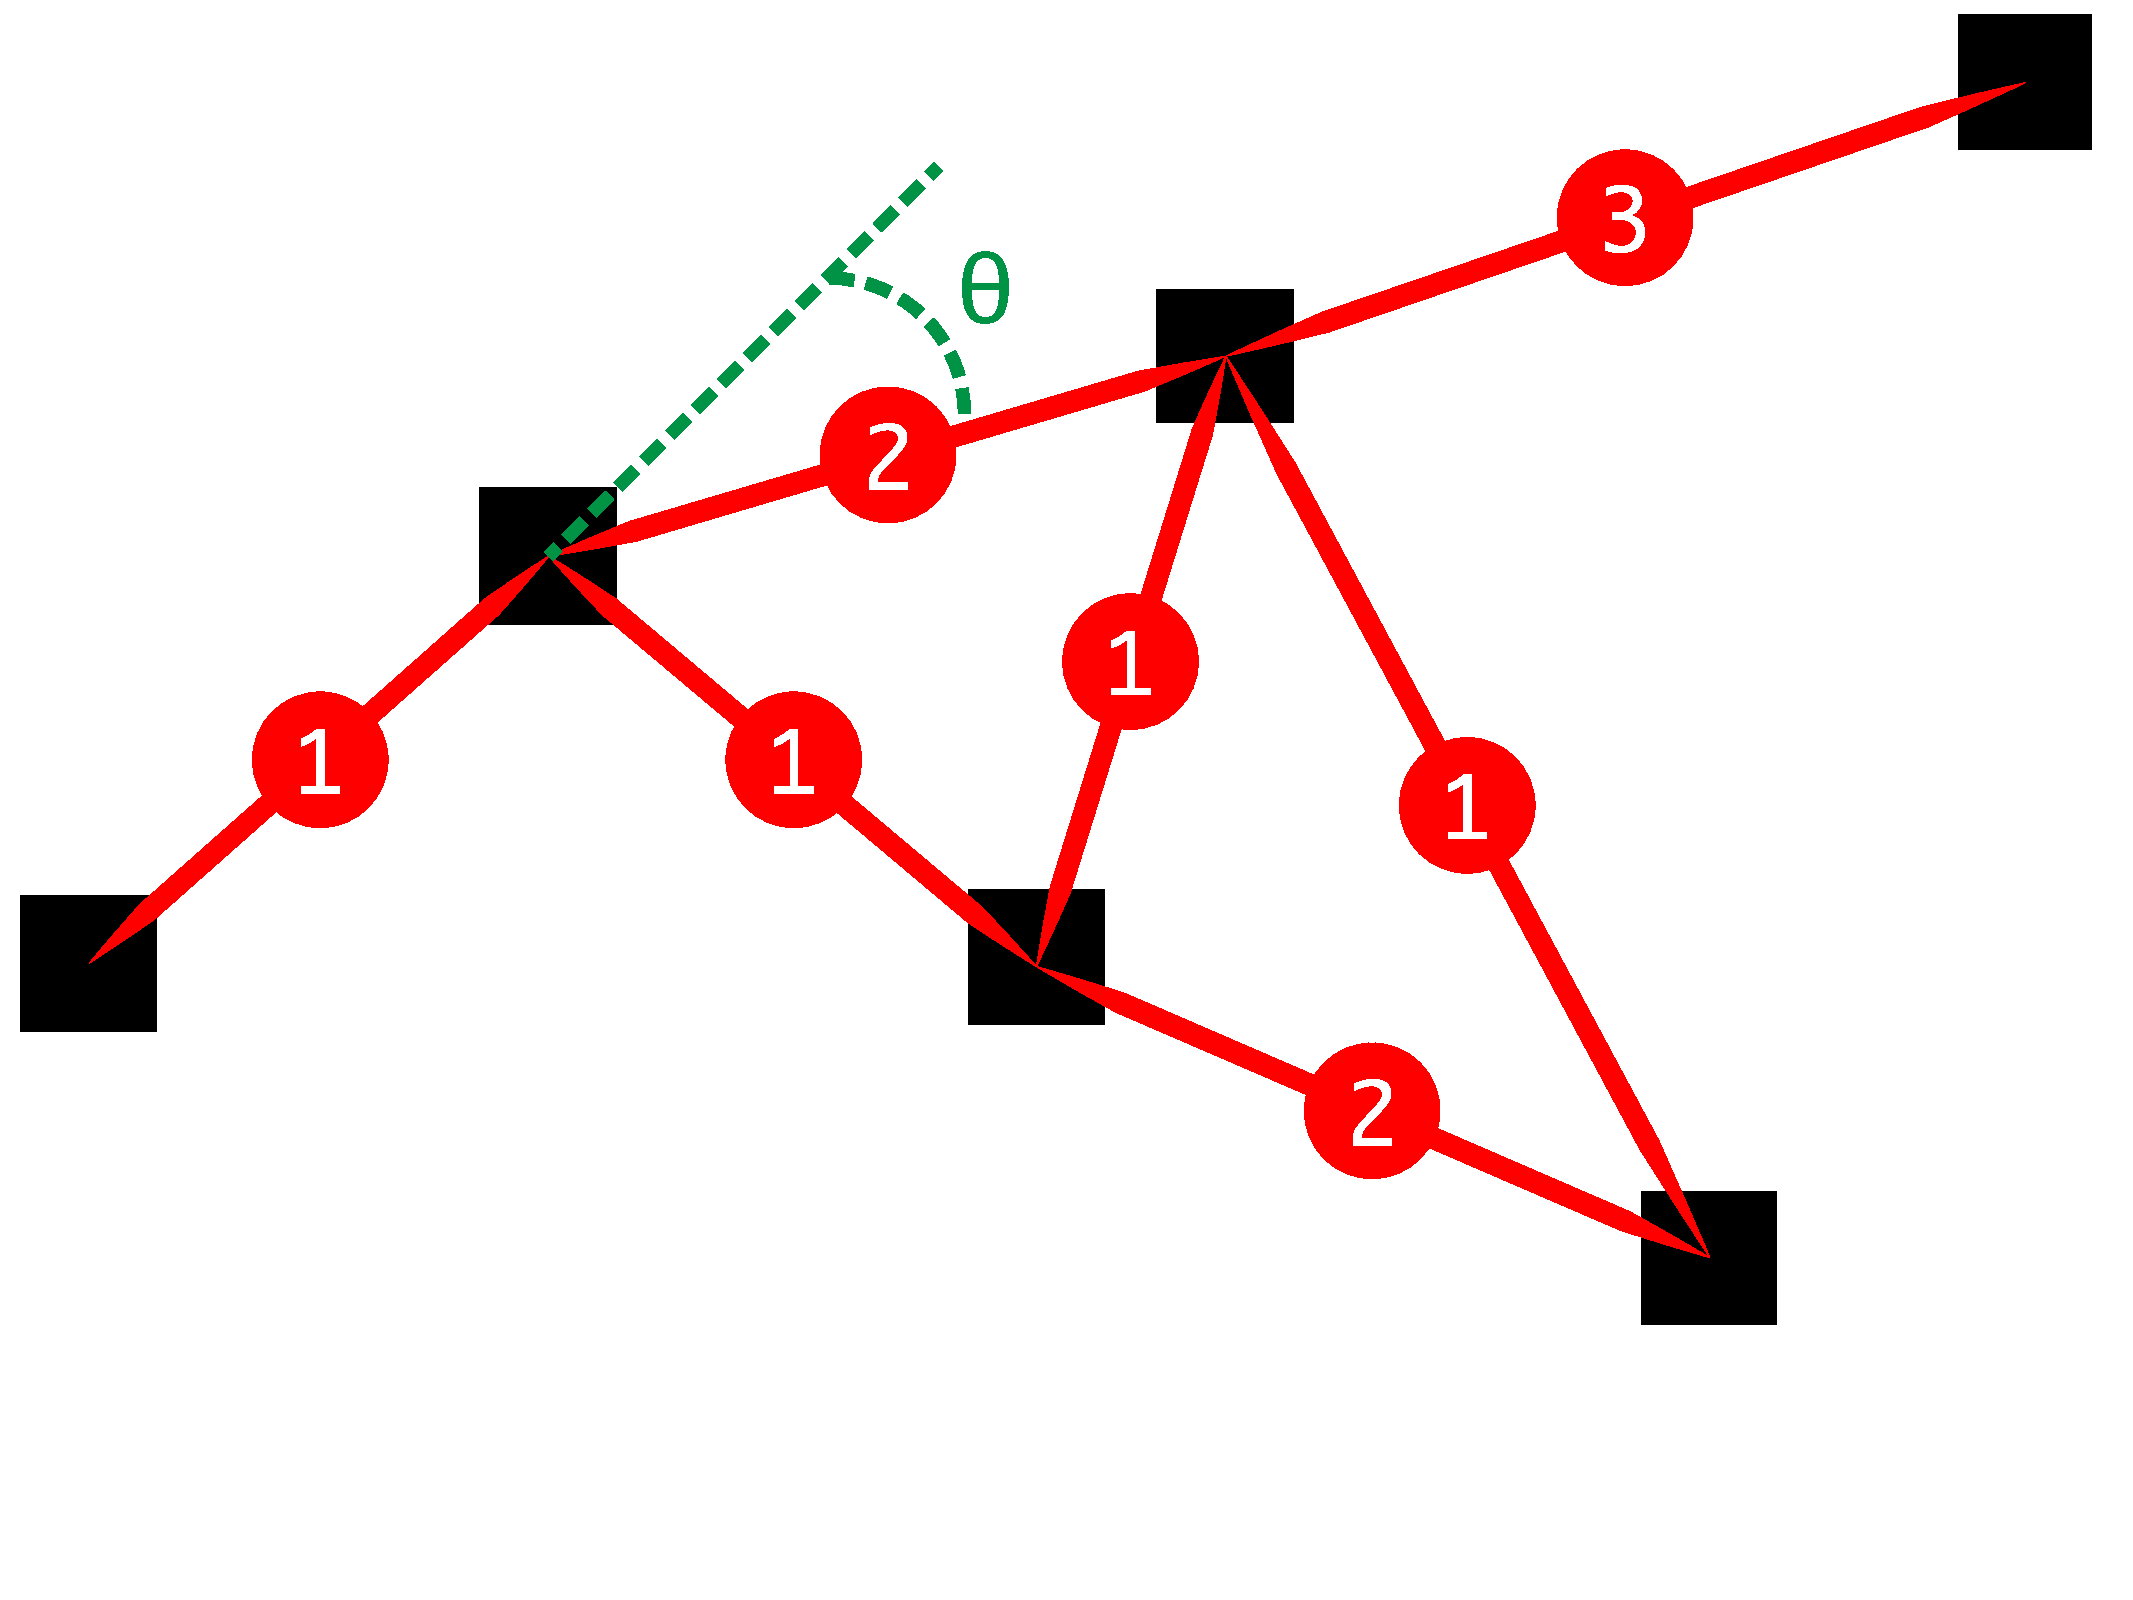
\includegraphics[width=0.3\textwidth]{chapters/cellularautomaton_images/ca-fig2-nolegend}
}
\subfigure[Output clustering]{\label{fig:cellularautomaton_run_output}
	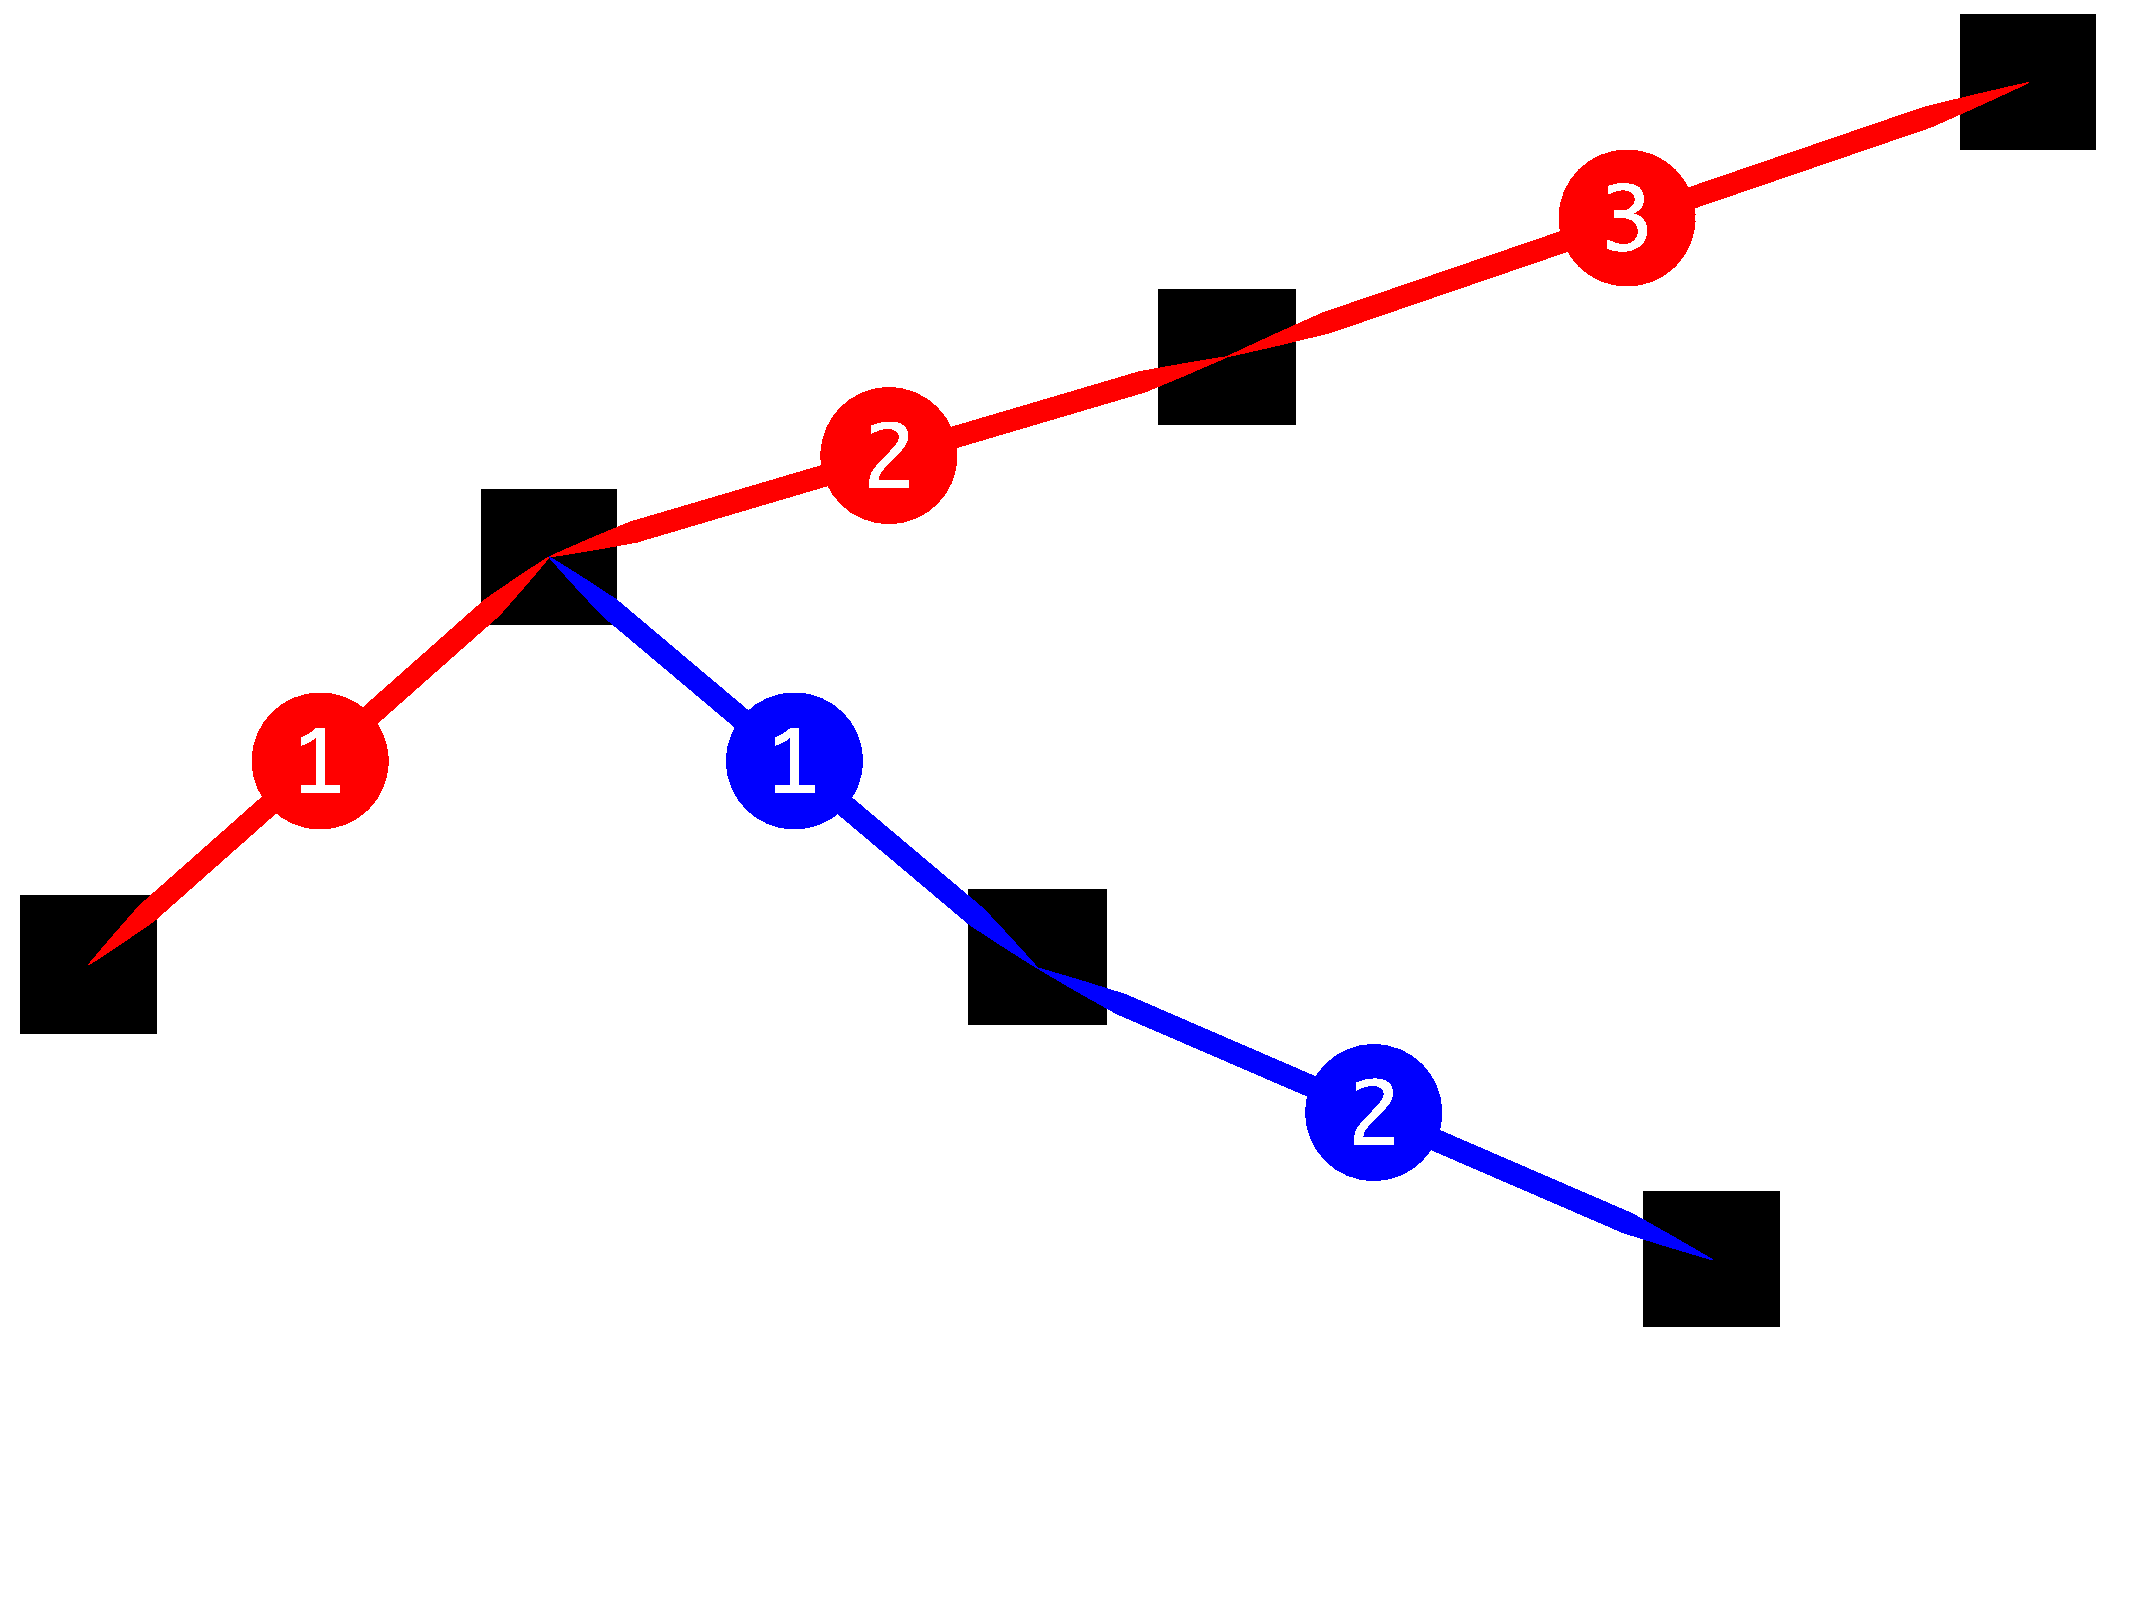
\includegraphics[width=0.3\textwidth]{chapters/cellularautomaton_images/ca-fig3-nolegend}
}

\caption[Initial and final states of a CA for track finding]{\label{fig:cellularautomaton_run}Illustration of the effects of the forward run of a \ac{CA} on a set of cells:\newline \subref{fig:cellularautomaton_run_initial} initial state with all cell values set to 1. \subref{fig:cellularautomaton_run_final} final state where cell values have been updated as per the forward step algorithm. Cell values now reflect the position of a cell in a straight line track. Cells which have no leftward neighbours consistent with the breaking angle $\theta$ retain the value 1. \subref{fig:cellularautomaton_run_output} track clusters are formed by following chains from high-valued to low-valued cells, while cells which are not part of a track are filtered out.}
\end{figure}

%% --------------------------------------------------
%% SUBSECTION: Reverse Run
%% --------------------------------------------------
\subsection{Reverse Run}\label{sec:cellularautomaton_reverse_run}
The reverse run extracts track clustering information from the final state of the \ac{CA}. The mapping of cells to a list of their leftward neighbours is retained, again for efficiency. Initially, all cells are considered as input to the reverse run. The reverse step algorithm is performed until no cells remain in the input list.

The reverse step algorithm proceeds as follows:
\begin{enumerate}
	\item Find the input cell with the highest valued state. Set as current cell.
	\item Create a new track candidate and add the current cell to it.
	\item While the current cell has value $> 1$:
	\begin{enumerate}
		\item Find a leftward neighbouring cell with state value 1 less than the current cell state.
		\item If multiple candidate cells exist, pick the one which makes the smallest angle with the current cell.
		\item Add this cell to the track candidate, and mark it as the new current cell.
	\end{enumerate}
	\item Remove allocated cells from the input list.
\end{enumerate}

Each reverse step follows a sequence of cells from a high-valued cell state to a cell with state 1, building a complete track candidate in the process. The reverse step algorithm runs until all track candidates have been extracted. Track candidates which contain only 1 cell are rejected as noise. The result of applying the reverse run algorithm is illustrated in figure \ref{fig:cellularautomaton_run_output}. Finally, the cells in each track candidate are unpacked to leave each track as a list of hits.

%% --------------------------------------------------
%% SUBSECTION: Postprocessing
%% --------------------------------------------------
\subsection{Postprocessing}\label{sec:cellularautomaton_postprocessing}
The \ac{CA} algorithm is considered to be complete at this point. Postprocessing stages are used to improve the results from the \ac{CA} based on its known properties.

The first stage involves uniquely assigning hits to tracks. The \ac{CA} makes unique assignments of cells to tracks, but since a hit can appear as an endpoint of multiple cells, it is possible that hits may appear multiple times across multiple tracks. The current strategy for unique hit assignment is to keep each hit with the longest track it is a member of, and remove it from any shorter tracks.

The second stage of postprocessing merges track segments together if they are compatible with being part of the same straight line. This is necessary because the CA tends to break tracks up at any site of complexity, including the primary vertex, decay vertices and delta electron production sites. In particular for $\mu$ tracks, it is useful to stitch together these segments to produce a single longer track. The merging algorithm is described in detail in section \ref{sec:cellularautomaton_merging}

%% --------------------------------------------------
%% SUBSECTION: Optimisation of parameters
%% --------------------------------------------------
\subsection{Optimisation of CA Parameters}\label{sec:optimisation_ca_parameters}
The algorithm presented is a general purpose reconstruction procedure for track-like objects in fine-grained detectors. In order to apply it to the data from a particular experiment or simulation, the parameters must be optimised somewhat to the environment in which it will be operating. One such optimisation is described in \citep{Back2013}, in which the parameters are tuned to maximise the product of hit-level efficiency times cluster-level purity. Hit-level efficiency is defined to be the number of hits visible in the CA output as a fraction of the total number of hits input, and is a measure of how well the CA retains data. Cluster-level purity is a measue of the contamination of each cluster, i.e. what proportion of the hits in a cluster originate from the same real track, i.e. a measure of the clustering capabilities of the algorithm. By maximising this product it was found that a wide range of CA parameters provide comparable results. Further optimisation then depends on the desired output from the CA, as well as experimental considerations such as the physics goals and operating energies.

Another optimisation is presented in section \ref{sec:long_two_track_events}, and in particular table \ref{table:ccqe-2tr-opt-results}. Here, the number of output tracks after the application of a merging procedure is used as a measure of the ability of the CA to produce the kind of clustering expected for the input data, which consists of two-track events with long tracks. Any use of the CA in a reconstruction chain requires optimisation of the parameters for the desired clustering, taking into account detector and experimental properties.

%% --------------------------------------------------
%% SECTION: Performance of the CA on Toy MC Events
%% --------------------------------------------------
\section{Performance of the \acl{CA} on Toy Monte Carlo Events}\label{sec:ca-toy-tracks}
The \ac{CA} was initially tested on a set of straight line tracks from a toy \ac{MC} generator which deposits charge from straight line segments in voxels of $1\mm\times1\mm\times1\mm$. The tracks are generated such that they have lengths between $200\mm$ and $300\mm$. Both tracks begin at point $(0, 0, 0)$, and the opening angle between the two tracks is fixed to some $\theta$. The events are then rotated so that the lines are distributed isotropically, but retain the fixed opening angle and start point. A thousand events were generated at each angle $\theta$ from $2\degree$ to $178\degree$ in $4\degree$ intervals.

The events were first charge weighted with a radius of $6.0\mm$, then scaled with a scale size of $3.0\mm$. The resulting hits were run through the cell generation process with a default cell generation radius of $6.0\mm$, maximum radius $15.0\mm$ (in unscaled units). The \ac{CA} algorithm itself was applied to each event in turn. The breaking angle was set to $\theta_\mathrm{max} = 10\degree$ and the resulting tracks were postprocessed with the track road merging algorithm with a cylinder radius of $5.0\mm$.\footnote{These parameters were chosen in order to maximise the number of correctly reconstructed events.}

%% --------------------------------------------------
%% SUBSECTION: Raw CA output
%% --------------------------------------------------
\subsection{Raw \acl{CA} Output}
The number of tracks found by the \ac{CA} as a function of angle is presented in figure \ref{fig:ca_toy_raw_trackcounts}. With 1000 events at each angle, and an input sample of events containing only two tracks, the number of interest is the efficiency for finding two tracks; that is, the number of events in which two clusters were found divided by the total number of events.% The two track efficiency is shown in figure \ref{fig:ca_toy_raw_twotrack_efficiency}.


\begin{figure}
\centering
% "Run8": CA Theta 10 deg, CW Radius 6 mm, Merging radius 5 mm
\resizebox{0.9\textwidth}{!}{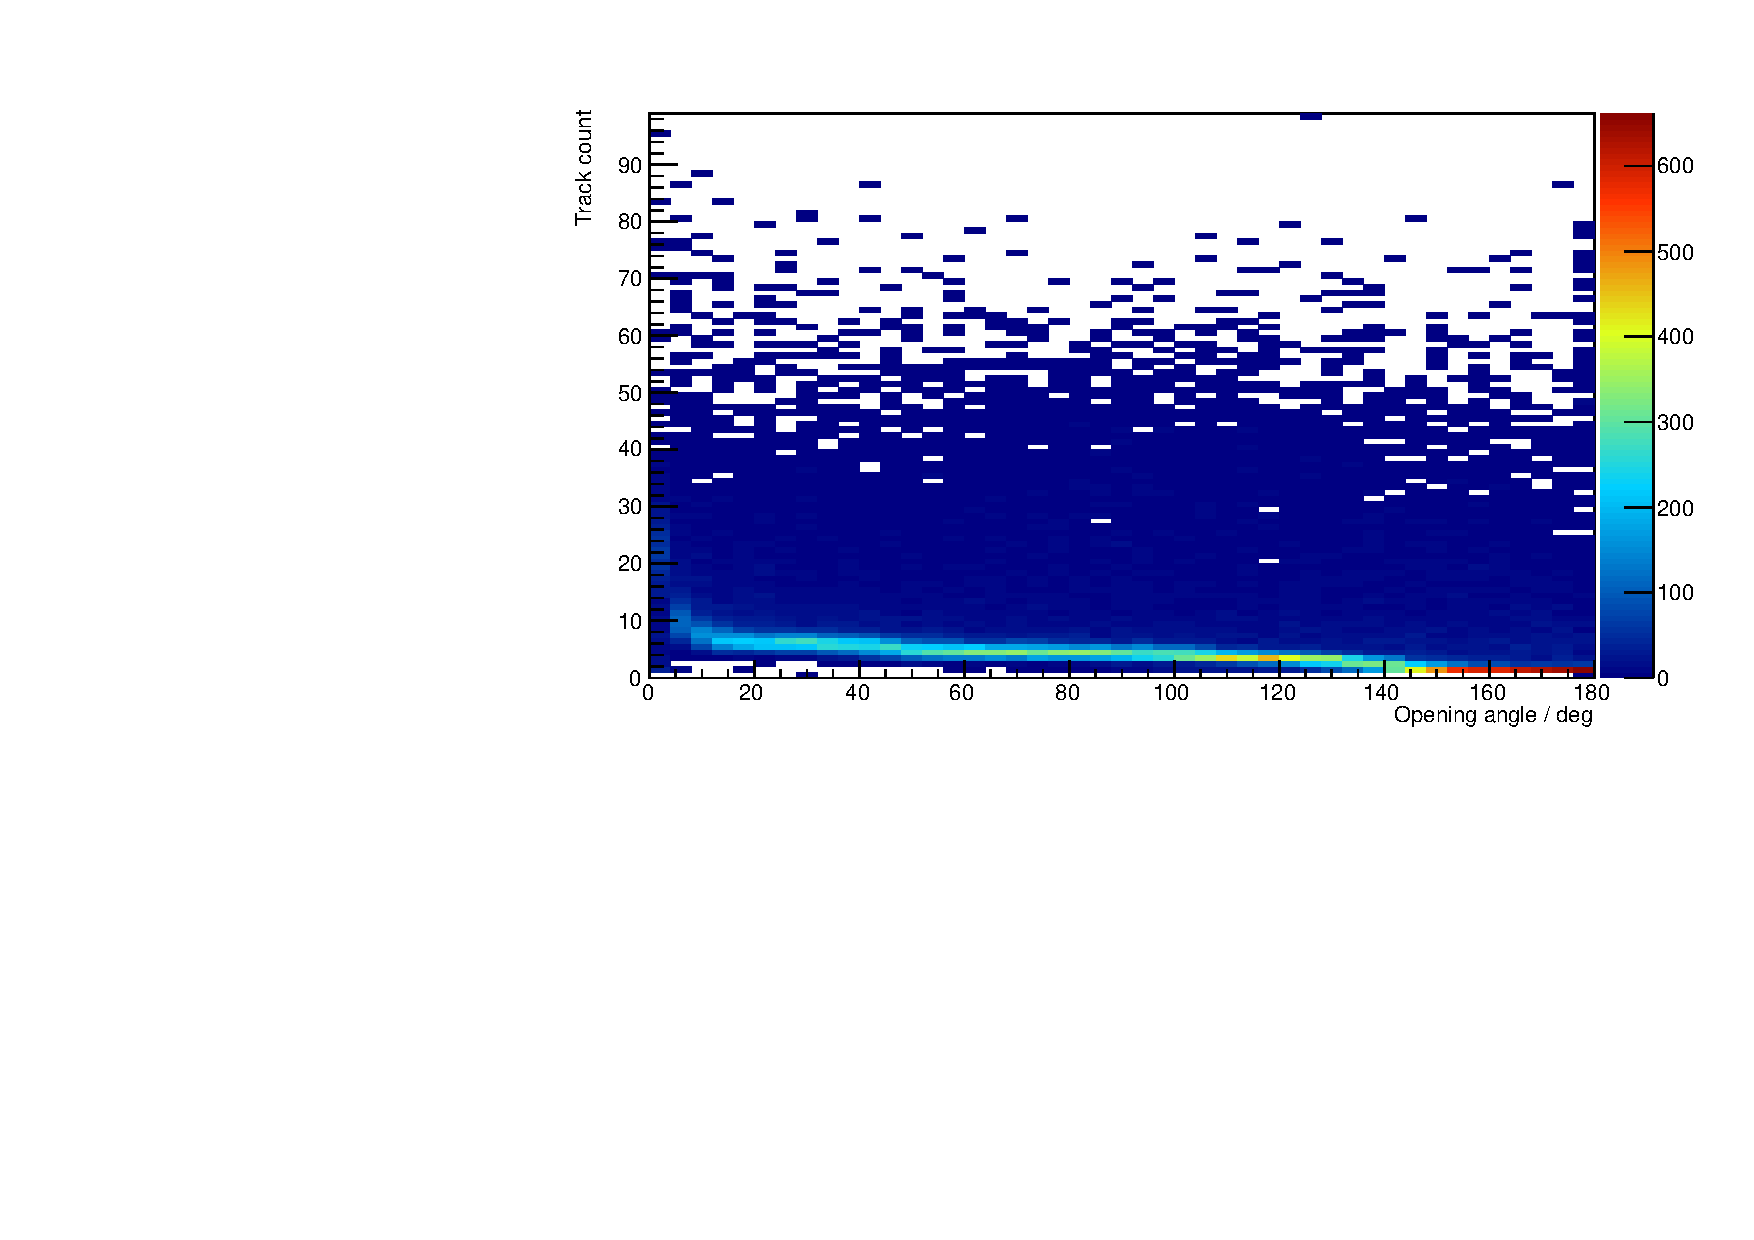
\includegraphics[angle=-90]{chapters/cellularautomaton_images/toy_raw_counts}}
\caption[Track count as a function of angle for raw CA operating on toy MC events]{\label{fig:ca_toy_raw_trackcounts}Number of tracks found as a function of opening angle for the raw \ac{CA} operating on two track events with a fixed opening angle. There are 1000 events per opening angle, and the events are rotated so as to be distributed isotropically. Large numbers of tracks are found in some cases due to geometric effects in the way the \ac{CA} operates. These can be merged back together with an appropriate merging algorithm.}
\end{figure}

\begin{figure}
\centering
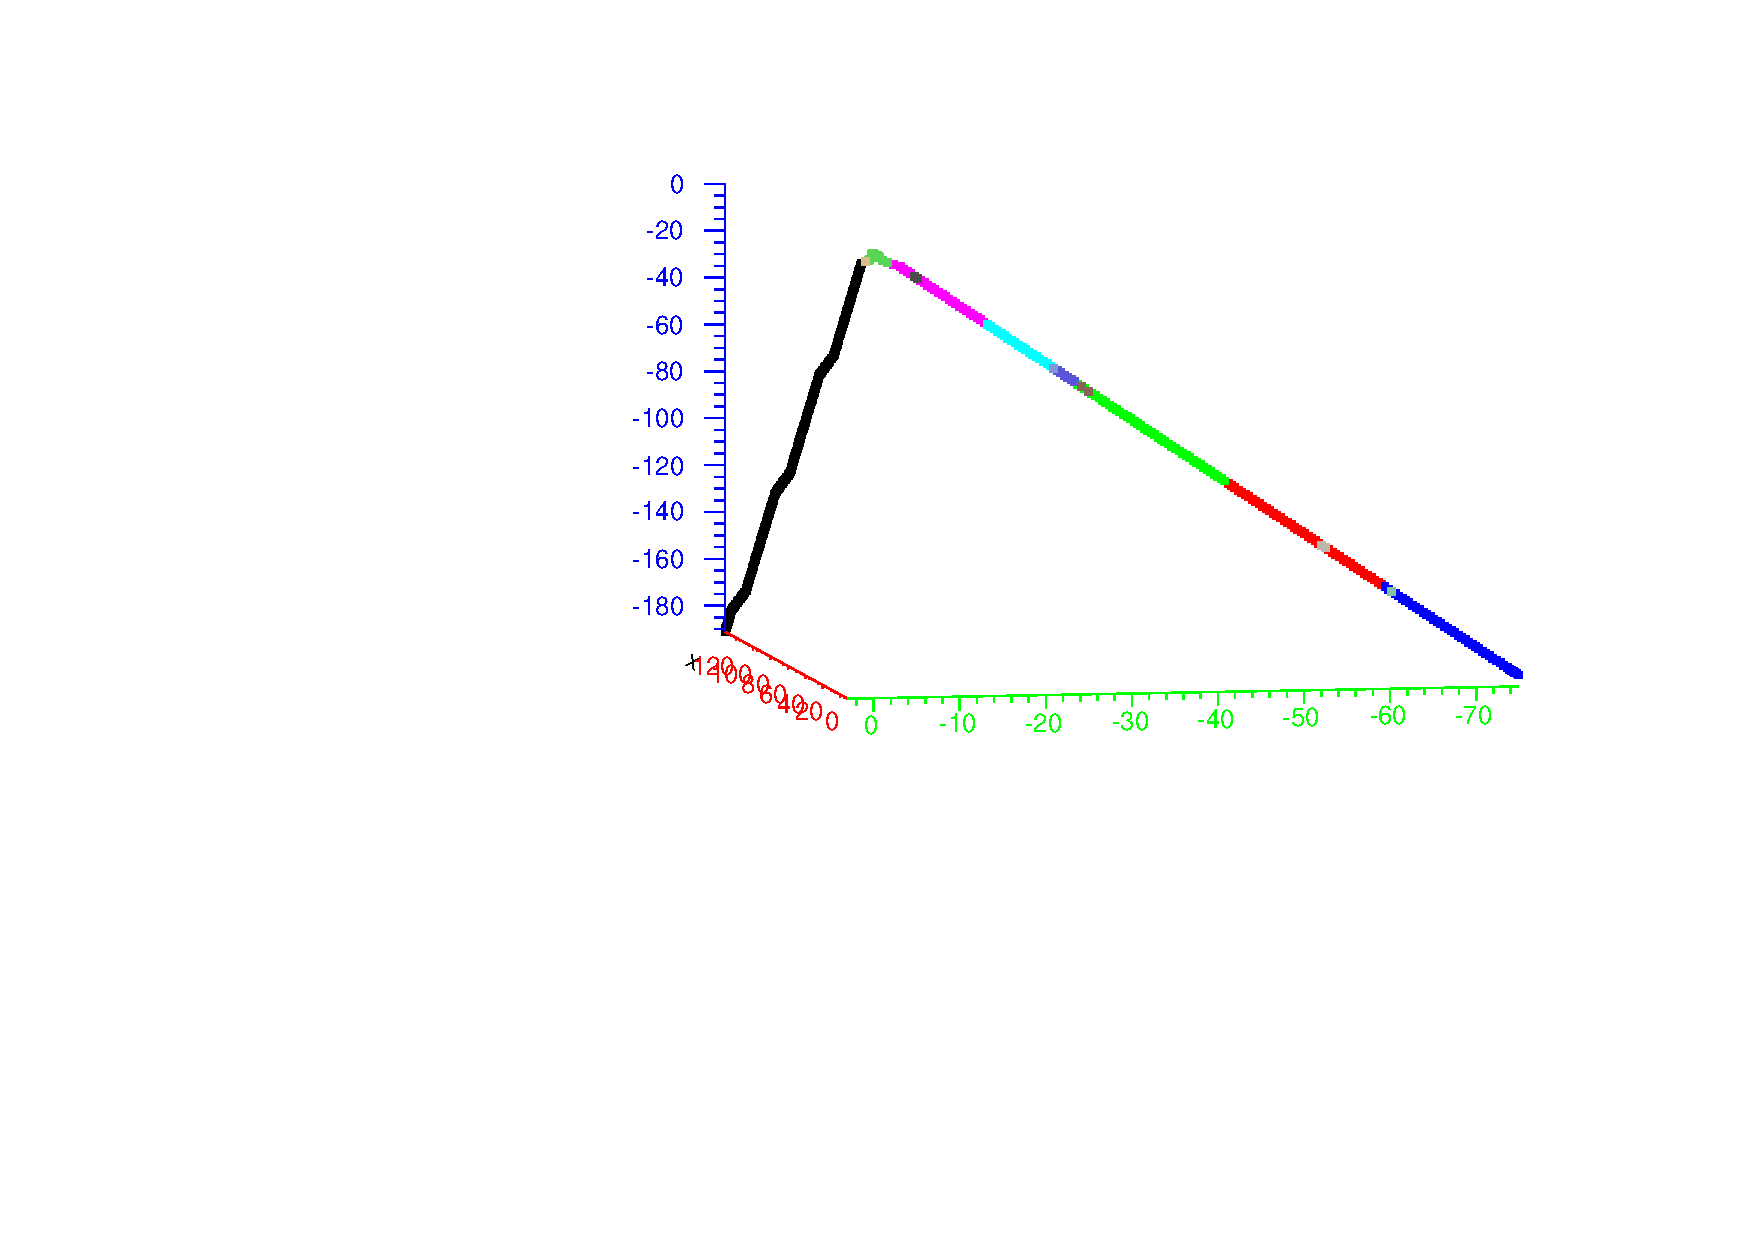
\includegraphics[angle=-90,width=0.8\textwidth]{chapters/cellularautomaton_images/openingangle-event_16-42deg}
\caption[Sample CA reconstruction of toy event with $42\degree$ opening angle]{\label{fig:ca-openingangle-sample-event-raw}Sample event from the toy track generator, with an opening angle of $42\degree$ between the two tracks. The cellular automaton clusters one track successfully, but produces several clusters (each coloured segment represents a cluster) along the length of the other due to the geometric effects of the voxellised data. It is important to note that each such cluster forms a segment along the line which is easy to merge together with the other segments, and that the segments include no hits that do not belong (i.e. hits from the other line).}
\end{figure}

While the raw performance of the \ac{CA}, characterised by the efficiency for finding two tracks, is poor, the resultant clustering typically provides long track candidates which can be used as key tracks in the track road merging process. Figure \ref{fig:ca-openingangle-sample-event-raw} shows the raw clusters output by the CA for one such event. Although there are many clusters, one track was successfully identified in its entirety, while the other is split into several shorter segments. Each segment is long enough to act as a seed point from which almost all of the segments may be merged together to recover the other long track. As such, the CA provides a significant advantage over applying a combinatoric approach using only track road algorithms, which is impractical given the large numbers of hits typically associated with a neutrino event in a \ac{LAr TPC}. The segmented track in this event is due to the CA being unable to cope with geometric effects introduced by the voxellised nature of the data. These effects tend to produce runs of linear structures, separated by a jump or step that the CA interprets to be a large angle between cells; one of the criteria for breaking a track in two. This is a natural outcome from the CA and is the desired effect when dealing with vertices and interaction points, so it cannot be ``tuned out''. The merging algorithm discussed below aims to compensate for these cases in which the track structure remains sufficiently linear to suggest that the desired outcome is one cluster, not two. Figure \ref{fig:ca-clustering-anomalies} shows one scenario in which the CA has produced several clusters from a single straight line due to the voxellised nature of the data. Here, the CA has found several straight line structures which must be merged to form a single line.

\begin{figure}
    \centering
    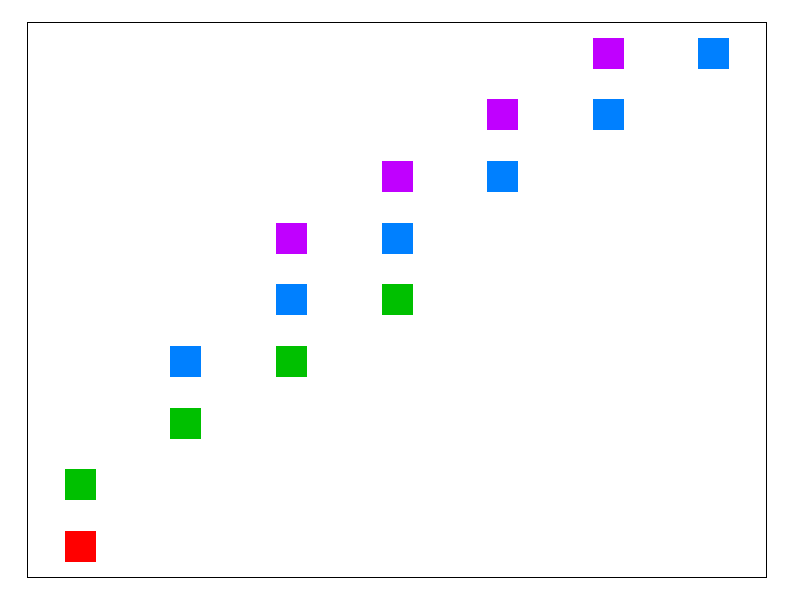
\includegraphics[width=0.5\textwidth]{chapters/cellularautomaton_images/clusters}
    \caption[Multiple reconstructed clusters for a single straight line]{\label{fig:ca-clustering-anomalies}Close-up of a track reconstructed by the CA algorithm, showing multiple straight line segments, each represented by a different colour. This is an side effect of the voxellised data format. The view shown is a zoomed region of the $xz$ projection of a line and each hit is positioned on a $3\mm$ square grid.}
\end{figure}

%% --------------------------------------------------
%% SUBSECTION: Performance of the CA with Merging
%% --------------------------------------------------
\subsection{Performance of the \acl{CA} with Merging}
When the merging process is applied, the track counts (figure \ref{fig:ca_toy_merged_trackcounts}) %and two track efficiency (figure \ref{fig:ca_toy_merged_twotrack_efficiency})
are considerably improved. The merging process tidies the events up, gathering together any track fragments and recombining them with the track they should belong to. In some cases, small track fragments remain, and while the modal number of tracks after merging is $2$, there is a long tail caused by a handful of events with significantly more tracks after merging. A simple range cut can be imposed to remove these remaining fragments.

\begin{figure}
\centering
% "Run8": CA Theta 10 deg, CW Radius 6 mm, Merging radius 5 mm
\resizebox{0.9\textwidth}{!}{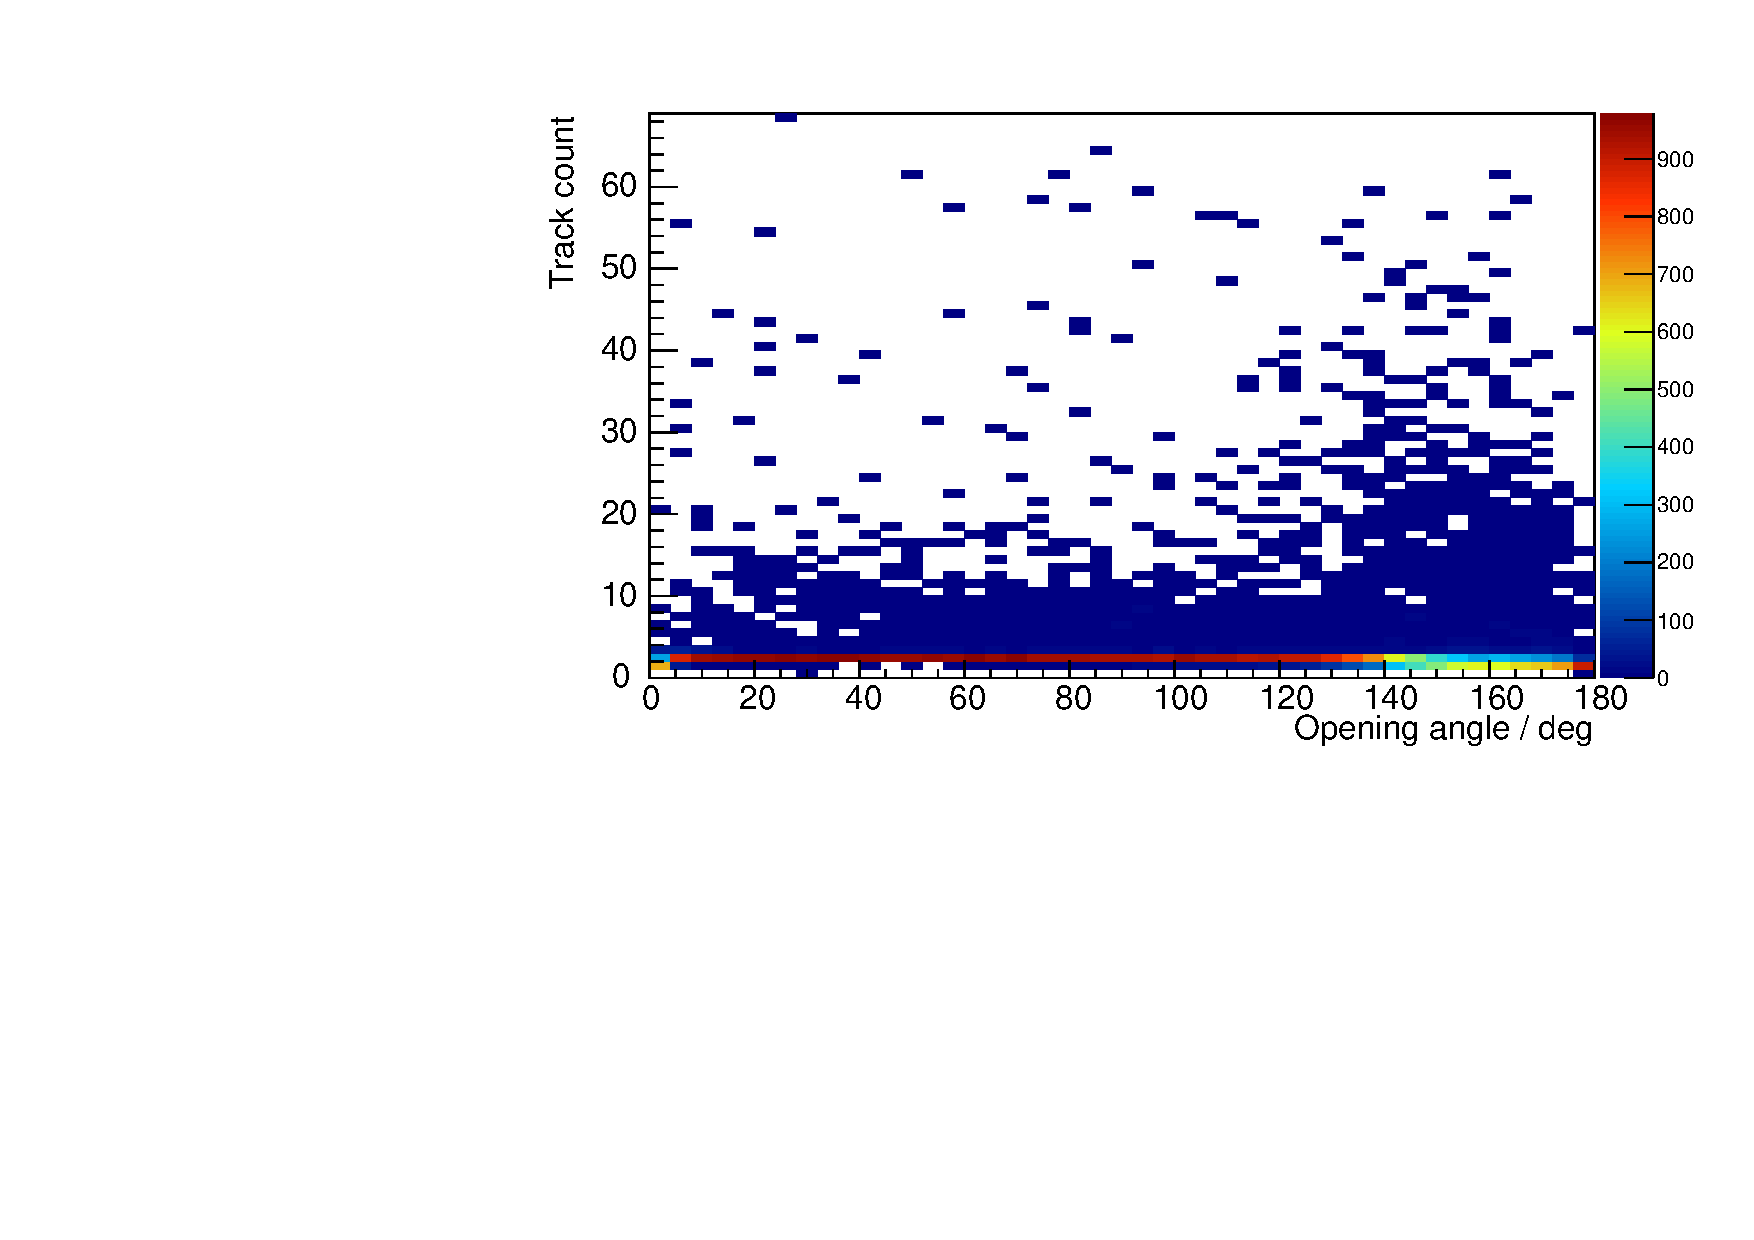
\includegraphics[angle=-90]{chapters/cellularautomaton_images/toy_merged_counts}}
\caption[Track count as a function of angle for CA with merging operating on toy MC events]{\label{fig:ca_toy_merged_trackcounts}Number of tracks found as a function of opening angle for the \ac{CA} with track road merging operating on two track events with a fixed opening angle. There are 1000 events per opening angle, and the events are rotated so as to be distributed isotropically. A small track fragment is usually left over, which can be removed with a suitable range cut.}
\end{figure}

%\begin{figure}
%\centering
%\resizebox{0.9\textwidth}{!}{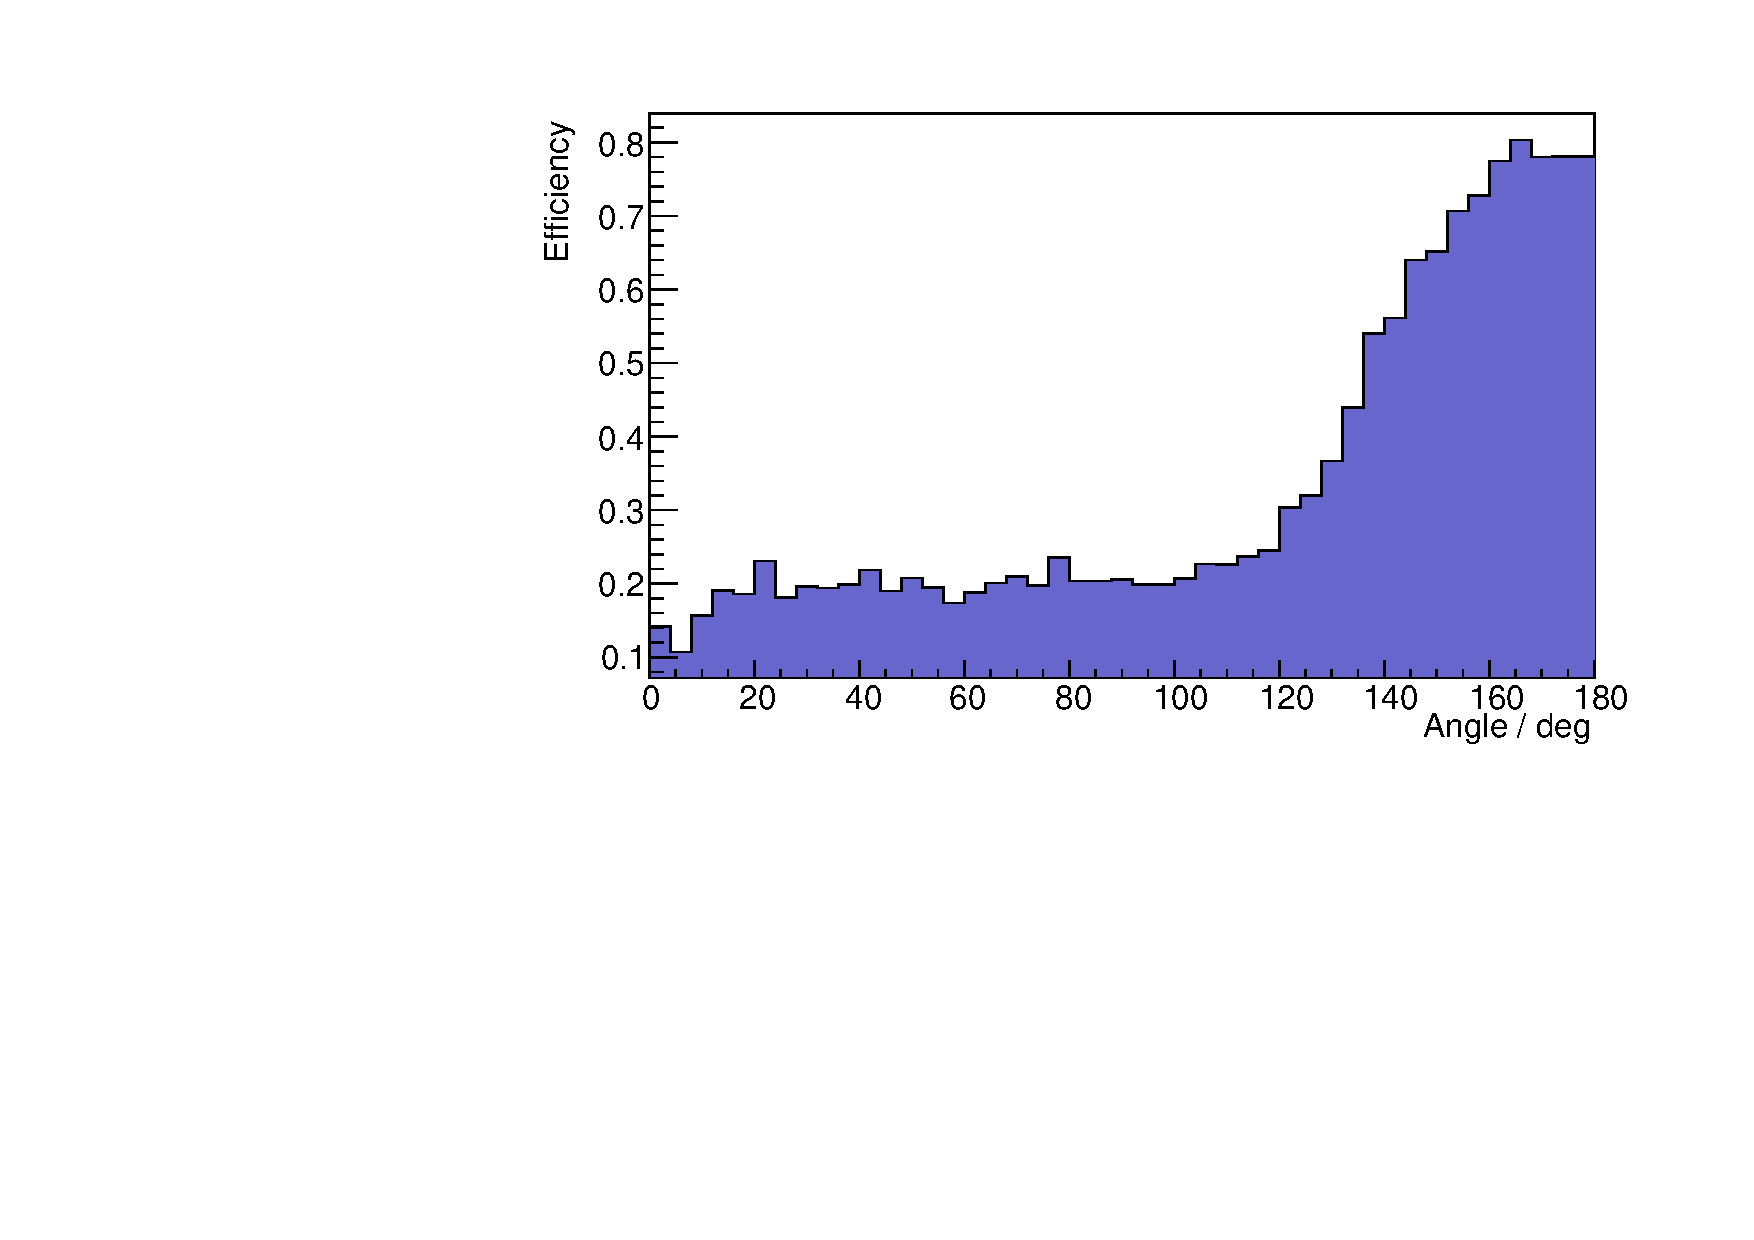
\includegraphics[angle=-90]{chapters/cellularautomaton_images/toy_merged_eff}}
%\caption[Efficiency for finding 2 tracks for CA with merging operating on toy MC events]{\label{fig:ca_toy_merged_twotrack_efficiency}Efficiency for finding two tracks in the \ac{CA} with track road merging operating on toy MC events with fixed opening angle, as a function of that angle. The efficiency is low due to small remnant fragments, which can be removed with a suitable range cut.}
%\end{figure}

%% --------------------------------------------------
%% SUBSECTION: Performance after a range cut
%% --------------------------------------------------
\subsection{Performance After a Range Cut}
After imposing a range cut of 20 hits (corresponding roughly to $20\mm$ or $4.2\MeV$ deposited by a minimum-ionising particle) the performance improves further. Now, the mean number of tracks (see figure \ref{fig:ca_toy_rcut_trackcounts}) is 2, giving a high two track reconstruction efficiency (figure \ref{fig:ca_toy_rcut_twotrack_efficiency}) for most opening angles. Above an opening angle of about $140\degree$ the \ac{CA} fails to cluster the two lines separately since the change in angle from one line to the next is now small and the \ac{CA} can smoothly travel across the join, resulting in a single output cluster. This is not symmetric with the case at an opening angle of $40\degree$, where the angle between the tracks is much sharper, and the \ac{CA} can easily distinguish the two. Efficiency curves are shown in fig. \ref{fig:ca_toy_rcut_twotrack_efficiency} at four different purity levels, defined on a hit level as the fraction of hits in a cluster which came from the same truth track. At $80\%$ and $85\%$ purity, the \ac{CA} performs with a high efficiency. This is reduced slightly for a requirement of $90\%$ purity, and substantially for a requirement of $95\%$ purity. The \ac{CA} can therefore be said to cluster simple topologies with very high efficiency and with reasonable purity, up to geometric opening angles of $140\degree$.

\begin{figure}
\centering
\resizebox{0.9\textwidth}{!}{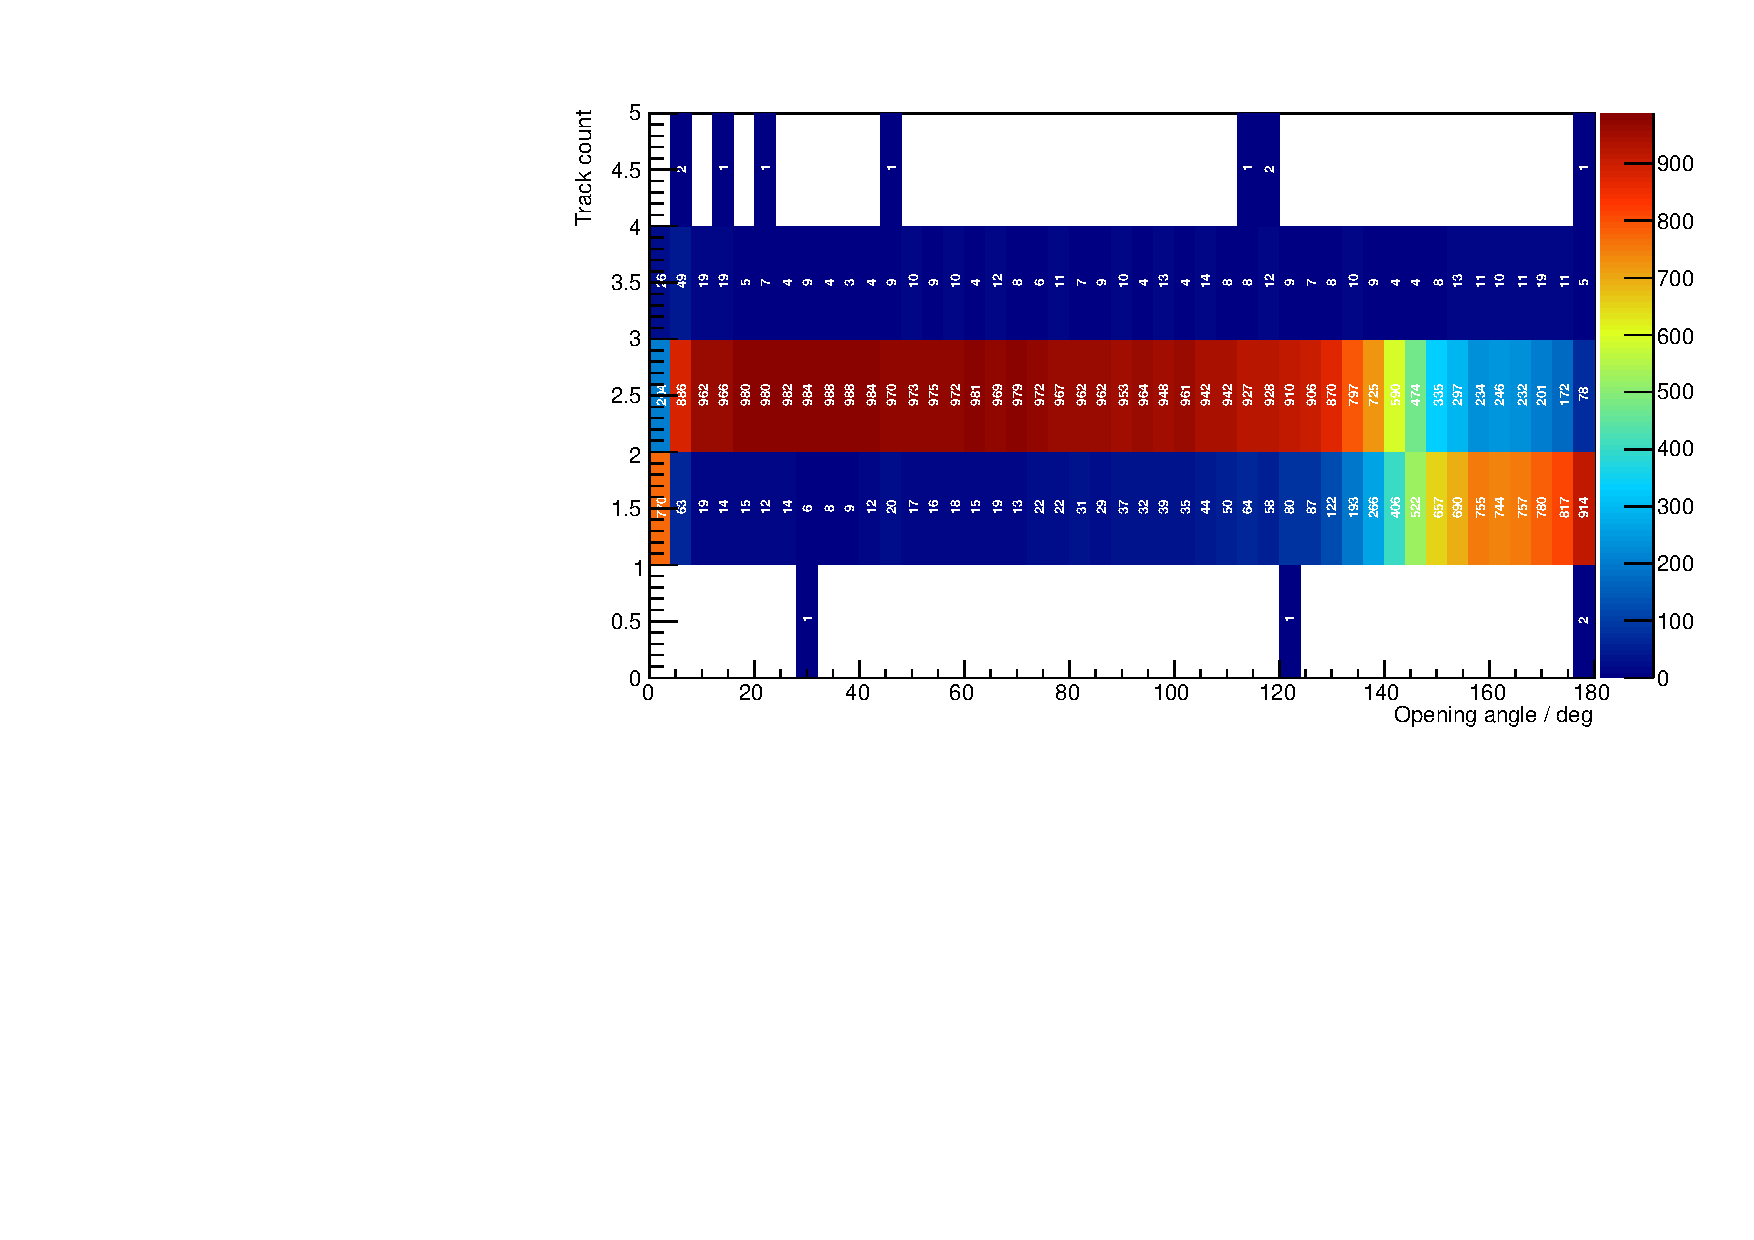
\includegraphics[angle=-90]{chapters/cellularautomaton_images/toy_rcut_counts}}
\caption[Track count as a function of angle for CA with merging and range cut operating on toy MC events]{\label{fig:ca_toy_rcut_trackcounts}Number of tracks found as a function of opening angle for the \ac{CA} with track road merging operating and a range cut of $20\mm$ on two track events with a fixed opening angle. There are 1000 events per opening angle, and the events are rotated so as to be distributed isotropically. The mean number of tracks found is now 2, dropping to 1 above $140\degree$ due to an inability of the \ac{CA} to distinguish this topology from that of a single continuous line.}
\end{figure}

\begin{figure}
\centering
\resizebox{0.9\textwidth}{!}{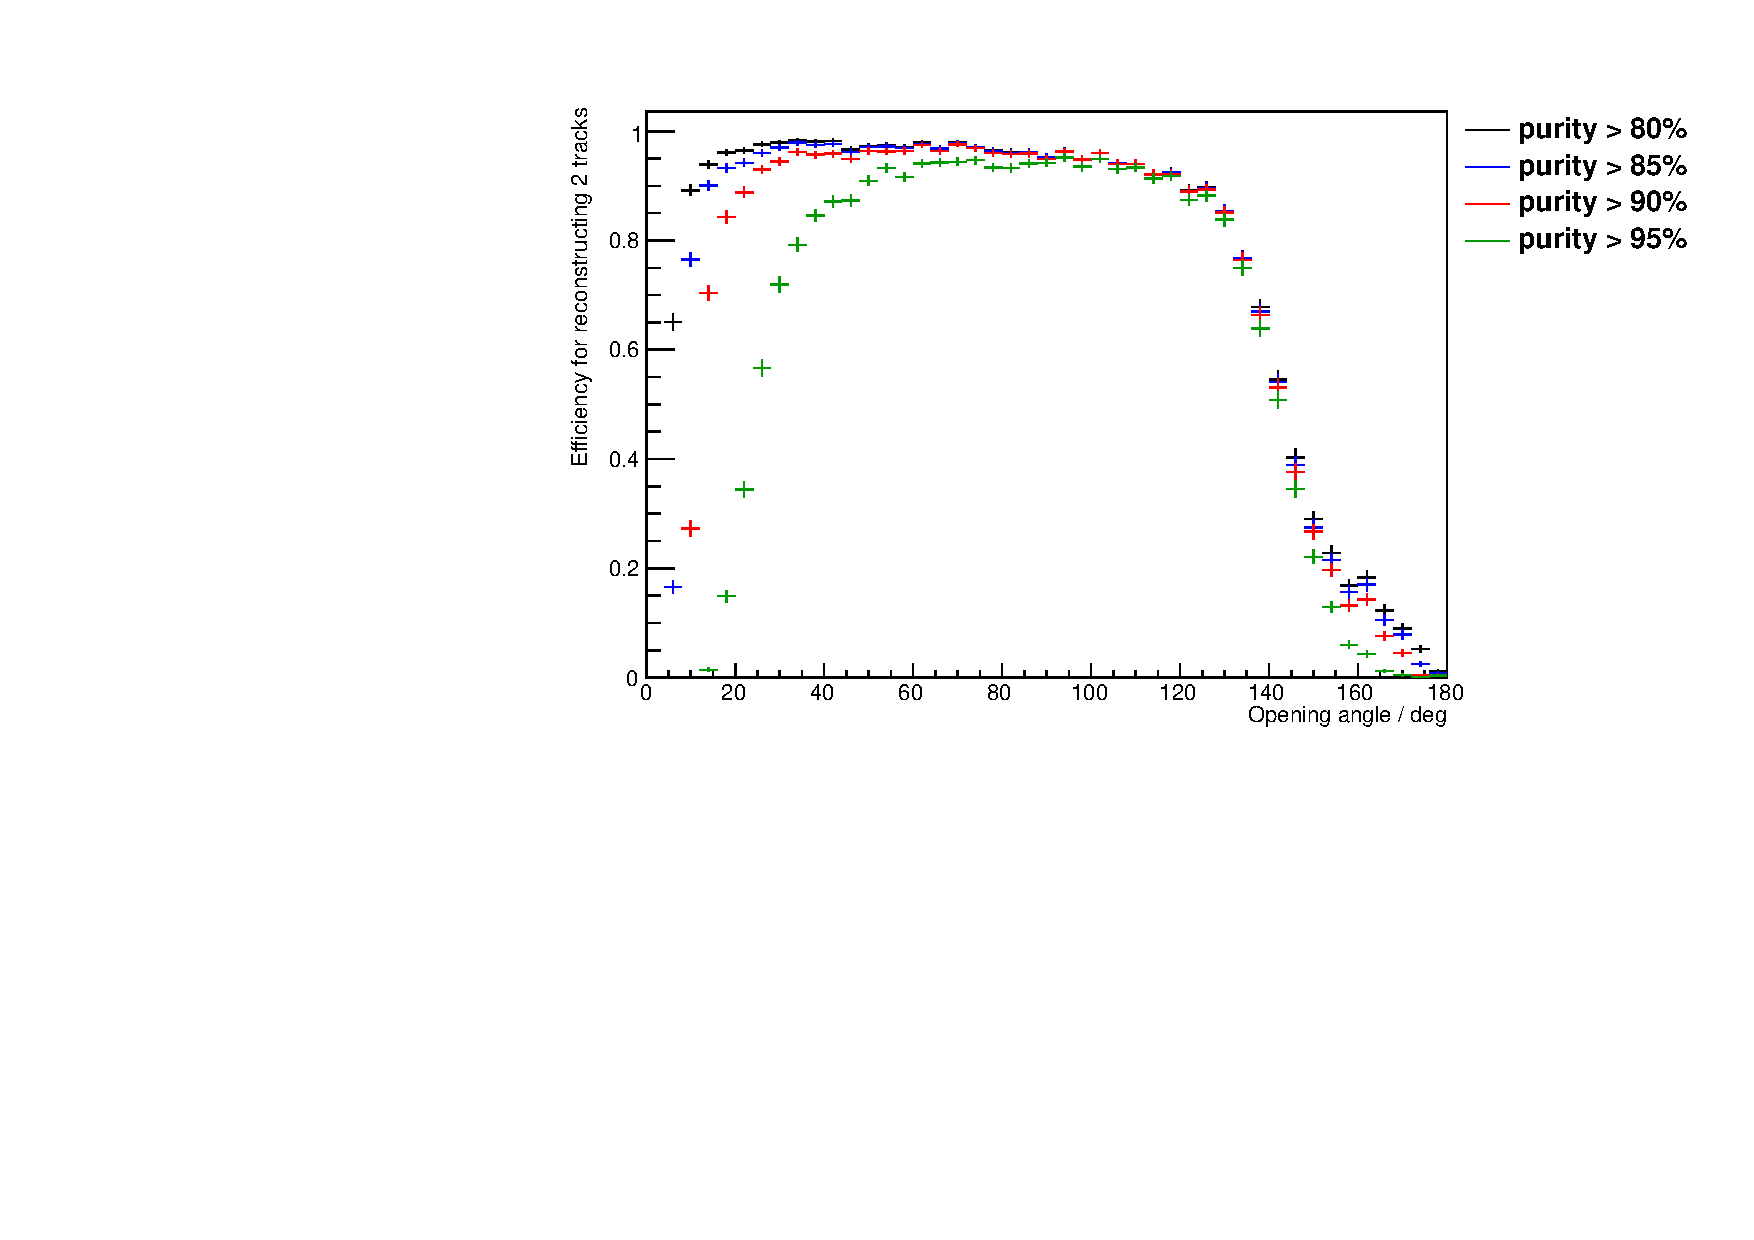
\includegraphics[angle=-90]{chapters/cellularautomaton_images/toy_rcut_eff}}
\caption[Efficiency for finding 2 tracks for CA with merging and range cut operating on toy MC events]{\label{fig:ca_toy_rcut_twotrack_efficiency}Efficiency for finding two tracks in the \ac{CA} with track road merging and a range cut of $20\mm$ operating on toy MC events with fixed opening angle, as a function of opening angle. Efficiency curves are plotted for four different purity cuts, requiring a minimum of $80\%$ (black), $85\%$ (blue), $90\%$ (red) and $95\%$ (green) purity in each track. The efficiency is high for almost all angles up to $140\degree$, beyond which the \ac{CA} is unable to distinguish the topology from that of a single continuous track.}
\end{figure}


\clearpage
%% --------------------------------------------------
%% SUBSECTION: Performance of the CA on Genie MC Events
%% --------------------------------------------------
\section{Performance of the \acl{CA} on Genie Monte Carlo Events}
The data for this section consists of neutrino events generated using Genie and tracked through a detector using Geant4, as described in chapters \ref{sec:genie} and \ref{sec:lamu} respectively. The reconstruction algorithm is applied first to charged current $\nu_\mu$ interactions producing $\ccqe$ final states (often referred to as \acl{CCQE} events), and then to charged current $\nu_\mu$ interactions producing $\ccpi$ final states.

\subsection{Charged Current $\nu_\mu \rightarrow \ccqe$ (CCQE)}
The Genie event generator was used to model the interactions of $0.77\GeV$ muon neutrinos on Argon nuclei. A sample was obtained of 1000 charged current interactions resulting in $\ccqe$ (only) final states. The resulting events were tracked through a liquid Argon TPC using Geant4 and the voxel data stored for analysis. Interactions of this type are of particular interest because they account for approximately 66\% of the interaction cross section at low energy and the two-body final state allows an accurate estimate of the muon neutrino energy to be made from the muon kinematics alone.

This data sample raises the possibility of attempting to optimise the \ac{CA} parameters for reconstructing neutrino events. Since it is a full simulation, the events will contain noise arising from delta electrons, hadronic reinteraction of the proton, muon decay and other physics processes. The truth information recorded for each event allows for the selection of a subset of this information, for example just the hits corresponding to energy deposited by the primary particles. In this way it is possible to optimise the algorithms based on more realistic data than in the toy study, but without including obviously difficult events.

\subsubsection{Long Two-Track Events}\label{sec:long_two_track_events}
In the first instance, events were selected in which both the proton and muon contained over 200 hits (corresponding approximately to a $20\cm$ straight line) and the hits from other particles were stripped from the event prior to running the \ac{CA}. The resulting events therefore contain two long tracks and nothing else. In a small number of cases, the event topology may make it difficult for the \ac{CA} to reconstruct these events correctly, e.g. if the muon and proton were produced almost back-to-back, or if either particle undergoes a large scatter along its trajectory, but for the most part these events should be reconstructed with two clusters in the \ac{CA} output.

A total of 483 events out of the sample of 1000 contain muon and proton tracks with over 200 hits each. Three parameters available in the reconstruction algorithms were varied and these 483 events processed with each permutation. The parameters are the \ac{CA} track angle $\theta$ ($10\degree$, $20\degree$ and $30\degree$), the charge weighting radius $R_{w}$ ($2.0\mm$, $5.0\mm$ and $10.0\mm$) and the track merging radius $R_m$ ($10\mm$, $20\mm$ and $30\mm$). The results of this optimisation are shown in table \ref{table:ccqe-2tr-opt-results}, which lists the number of events reconstructed with one, two or three tracks against the reconstruction parameters used. The results are sorted by the number of events reconstructed with two tracks. The largest number of two-track events are returned from the algorithm when used with parameters $\theta=10.0\degree$, $R_w=5.0\mm$ and $R_m=30.0\mm$. These parameters yield 345 two-track events, corresponding to $71.4\%$ of the input sample. In addition, these parameters give a low number of one- and three-track events.

\begin{table}
\centering
\begin{tabular}{*{6}{r}}
$\theta$ ($\degree$) & $R_w$ ($\mm$) & $R_m$ ($\mm$) & $\phantom{000} $$N_1$  & $\phantom{000}$ $N_2$  & $\phantom{000}$ $N_3$  \\
\hline
\hline
10.0  & 5.0   & 30.0  & 59   & 345  & 72 \\
10.0  & 5.0   & 20.0  & 43   & 341  & 84 \\
10.0  & 10.0  & 30.0  & 91   & 335  & 53 \\
10.0  & 5.0   & 10.0  & 35   & 331  & 70 \\
10.0  & 10.0  & 20.0  & 76   & 331  & 66 \\
10.0  & 10.0  & 10.0  & 67   & 327  & 62 \\
20.0  & 5.0   & 30.0  & 109  & 305  & 62 \\
20.0  & 5.0   & 20.0  & 94   & 305  & 70 \\
20.0  & 2.0   & 30.0  & 64   & 302  & 109 \\
20.0  & 5.0   & 10.0  & 85   & 301  & 55 \\
20.0  & 2.0   & 20.0  & 49   & 301  & 114 \\
20.0  & 2.0   & 10.0  & 38   & 293  & 98 \\
30.0  & 2.0   & 30.0  & 101  & 288  & 87 \\
30.0  & 2.0   & 20.0  & 88   & 288  & 89 \\
30.0  & 2.0   & 10.0  & 79   & 279  & 77 \\
20.0  & 10.0  & 30.0  & 196  & 237  & 46 \\
20.0  & 10.0  & 20.0  & 189  & 231  & 53 \\
20.0  & 10.0  & 10.0  & 188  & 217  & 56 \\
30.0  & 5.0   & 30.0  & 206  & 210  & 59 \\
30.0  & 5.0   & 20.0  & 198  & 204  & 67 \\
30.0  & 5.0   & 10.0  & 195  & 195  & 55 \\
10.0  & 2.0   & 30.0  & 28   & 170  & 246 \\
30.0  & 10.0  & 30.0  & 276  & 163  & 40 \\
30.0  & 10.0  & 20.0  & 271  & 157  & 45 \\
30.0  & 10.0  & 10.0  & 271  & 143  & 50 \\
10.0  & 2.0   & 20.0  & 16   & 97   & 285 \\
10.0  & 2.0   & 10.0  & 4    & 56   & 189 \\
\hline
\end{tabular}
\caption[Optimisation of Cellular Automaton reconstruction parameters]{\label{table:ccqe-2tr-opt-results}Optimisation of reconstruction parameters in the \ac{CA} for reduced CCQE events (see text for details). Data is shown for the number of events reconstructed as containing one, two or three tracks ($N_1$, $N_2$ and $N_3$) for different combinations of the track opening angle $\theta$, the charge weighting radius $R_w$ and the track merging radius $R_m$. Entries are sorted by the number of events reconstructed with two tracks ($N_2$), largest first. Each set of parameters was used to process the same 483 events. Events with more than three reconstructed tracks are not shown.}
\end{table}

While the number of tracks found in an event is one metric of the quality of the reconstruction, it is also important to consider \emph{hit efficiencies} and \emph{track purities}.
\begin{description}
    \item[Hit efficiency:] A measure of how much of the original event data is retained. Hits that are present in any output cluster, divided by the number of input hits. High hit efficiency means that the algorithm is not throwing away many hits, which makes subsequent energy calculations easier. Due to the nature of the \ac{CA}, the algorithm will necessarily throw away some hits but the track structures should remain and lost hits can be retrieved with track-road style merging applied to the original data, rather than to a cluster, if required.
    \item[Track purity:] A measure of how selective the clustering is. An output cluster will contain hits from one or more truth tracks. The track purity is the largest number of contributing hits from a single track, divided by the total number of hits. High purity means that the \ac{CA} clustered mostly hits from a single trajectory together. This is extremely important, though the purity is often diluted by hits from e.g. delta electrons produced along the length of a muon track, but clustered with it.
\end{description}

Figure \ref{fig:ca-ccqe-reduced-eff-pur-efficiency} shows the hit efficiency and figure \ref{fig:ca-ccqe-reduced-eff-pur-purity} track purity results from the analysis performed with $\theta=10\degree$, $R_w=5.0\mm$ and $R_m=30.0\mm$. The efficiency drops slightly with track length, most likely due to increased scattering as the particle that produced the track loses energy and slows down. The \ac{CA} will struggle with situations where the scattering angles exceed the track breaking angle $\theta$, and will produce many short track segments, each of which will be filtered out in subsequent stages unless they can be merged together. The track purity remains over $90\%$ for all track lengths, indicating that the \ac{CA} with these parameters is capable of differentiating extremely well between unrelated trajectories.

\begin{figure}
    \centering
    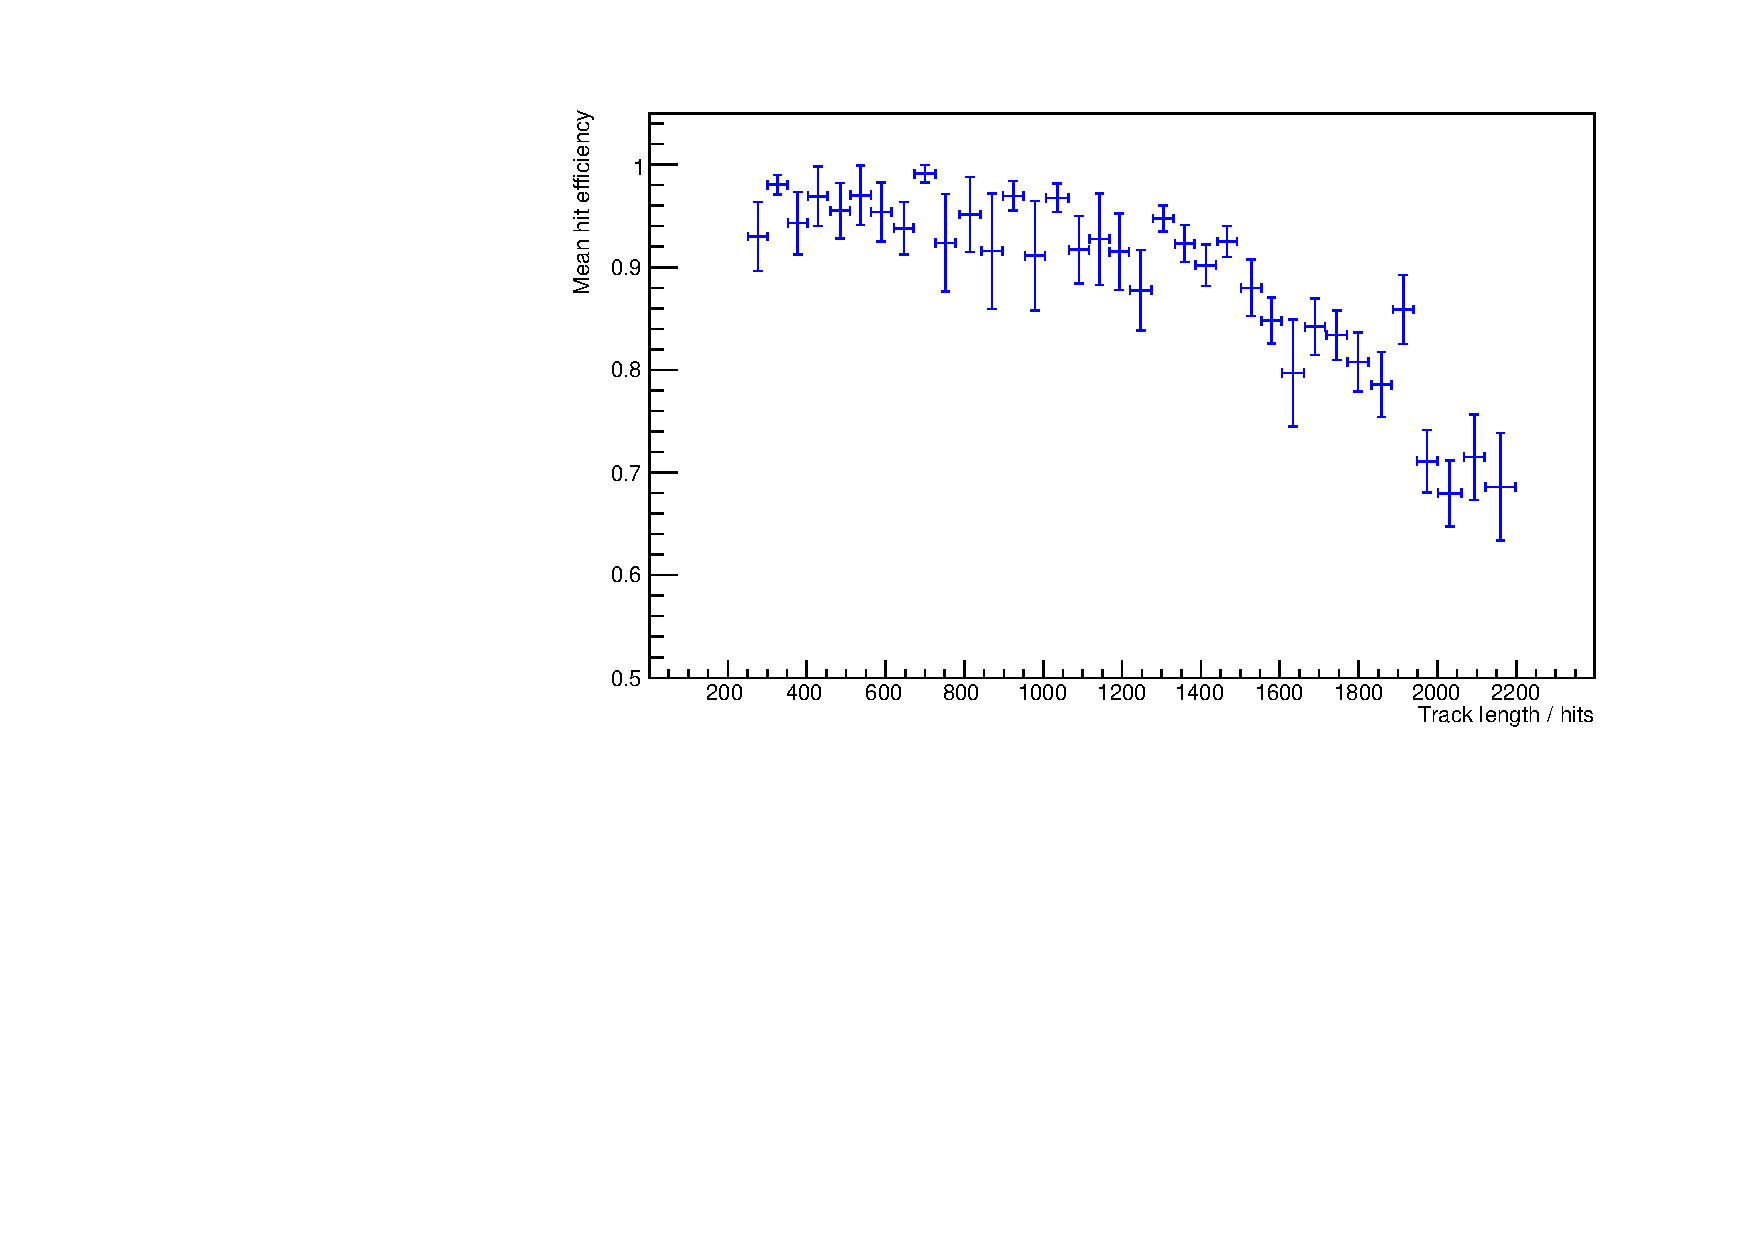
\includegraphics[angle=-90,width=0.9\textwidth]{chapters/cellularautomaton_images/ccqe-reduced-hit-efficiency}
    \caption[Hit efficiency for CA operating on long muon and proton tracks]{\label{fig:ca-ccqe-reduced-eff-pur-efficiency}Hit efficiency for the \ac{CA} operating on long muon and proton tracks from CCQE events. The hit efficiency is high, but drops as a function of track length, indicating that the \ac{CA} is not capable of retaining all hits for long tracks, most likely due to increased scattering.}
\end{figure}

\begin{figure}
    \centering
    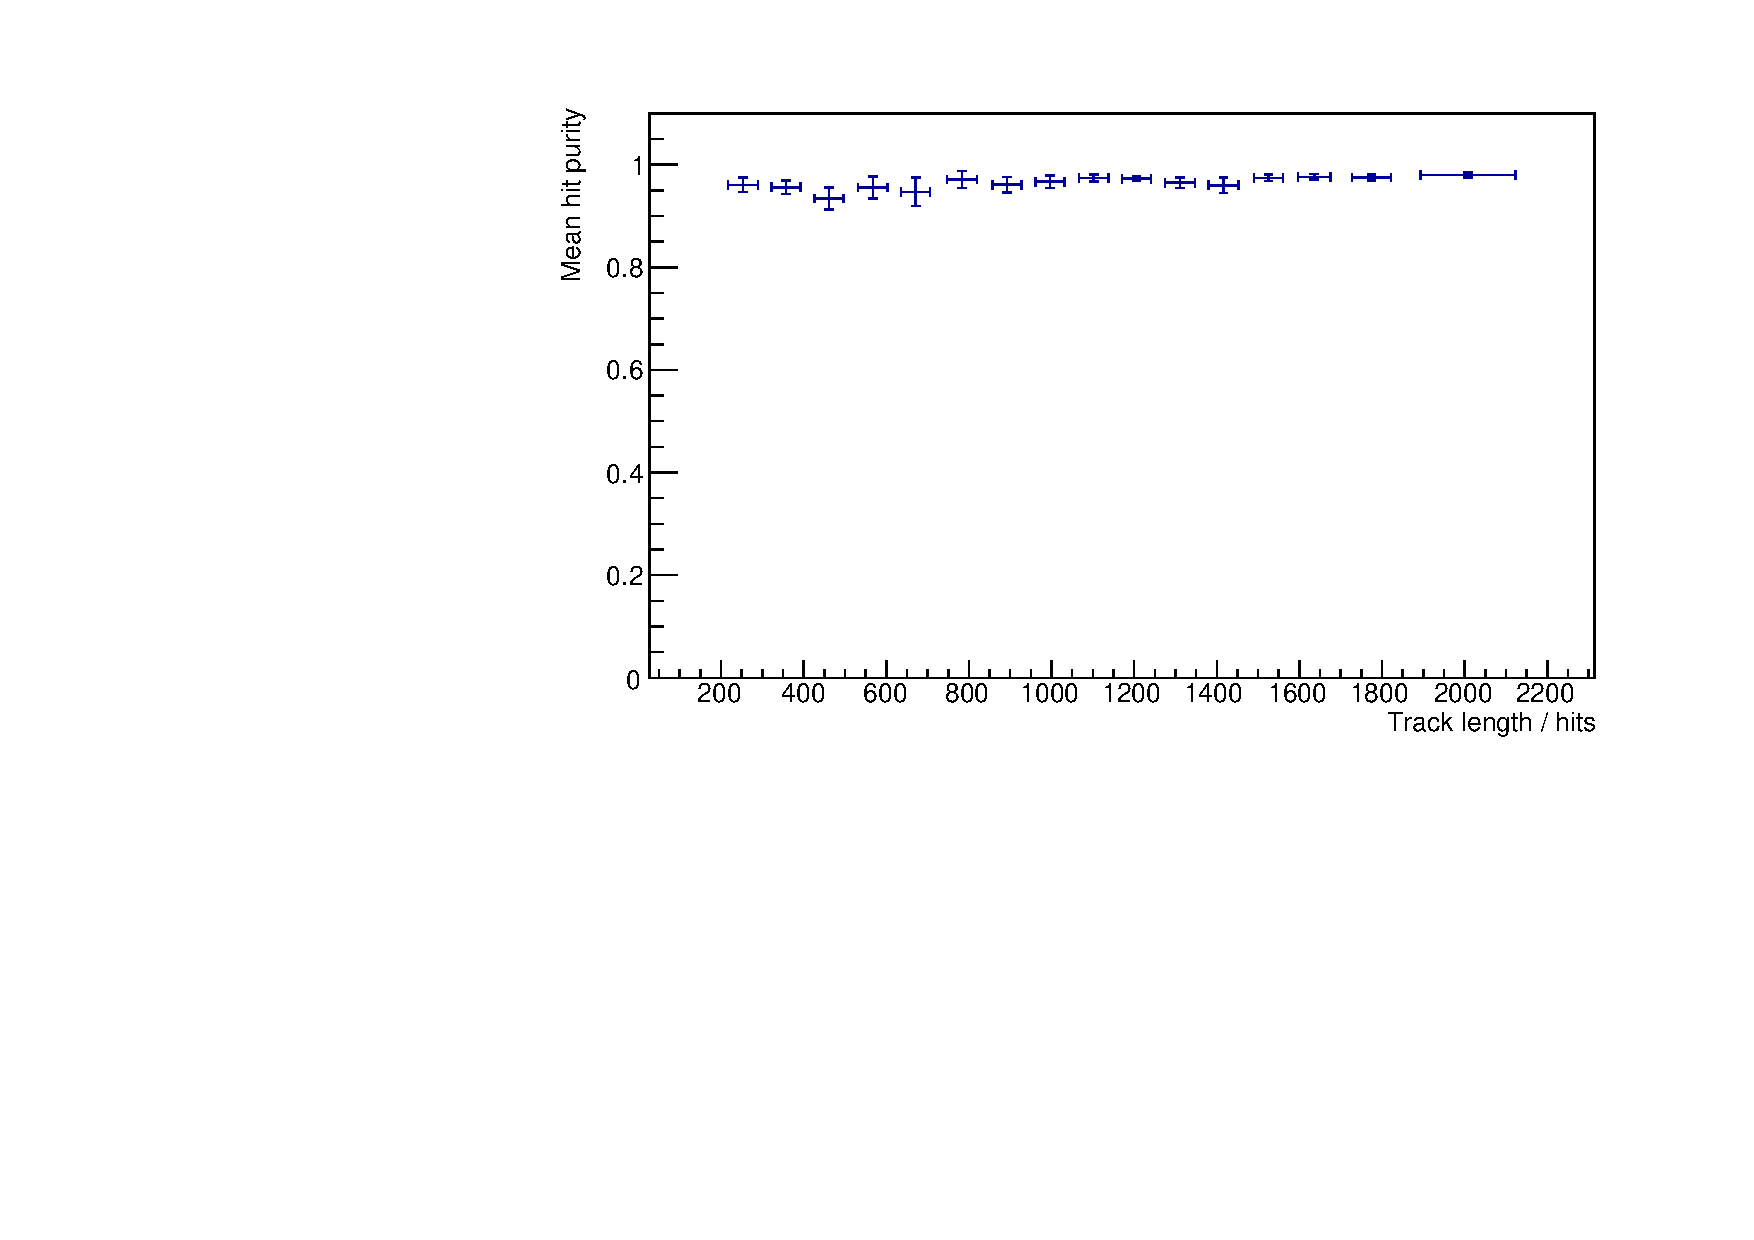
\includegraphics[angle=-90,width=0.9\textwidth]{chapters/cellularautomaton_images/ccqe-reduced-cluster-purity}
    \caption[Track purity for CA operating on long muon and proton tracks]{\label{fig:ca-ccqe-reduced-eff-pur-purity}Track purity for the \ac{CA} operating on long muon and proton tracks from CCQE events. The purity is over $90\%$ for all track lengths, indicating that the \ac{CA} is capable of separating hits resulting from different particles extremely well.}
\end{figure}

\subsubsection{Full Reconstruction}
Having attempted to optimise the parameters on a reduced dataset where two reconstructed tracks are expected, the performance of the \ac{CA} can be assessed when run against the full simulated events. Here, a much smaller range cut of 20 hits is applied. Events containing proton tracks with fewer than 20 hits are not processed, and in the remaining events all objects with fewer than 20 hits are cut out of the data before reconstruction. A 20 hit track corresponds approximately to a $20\mm$ trajectory, or an energy deposit of $4.2\MeV$, based on a minimum-ionising particle depositing $2.1\MeV \cm^{-1}$. Such values can be considered as realistic energy thresholds in any liquid Argon TPC, and the presence of tracks in the simulated data with such short range adds noise that would simply not be seen in a real detector. Following the 20 hit range requirement on protons, 878 events of the 1000 event sample survive for reconstruction. 

Because of this relaxation of the initial range cuts, and because the full event data is now included, the results are expected to be poorer than those for the case presented above. In particular, the noise introduced by delta electrons will serve to pull the \ac{CA} off course as it follows long tracks, and the decay products may themselves contribute additional tracks which can be reconstructed. We should not, therefore, expect the mean number of reconstructed tracks to be two.

Figure \ref{fig:ca-ccqe-full-trackcounts} shows the distribution of reconstructed track counts. Of the 878 events, 420 ($47.8\%$) had two reconstructed tracks, while a further 270 ($30\%$) had three reconstructed tracks and a further 86 events ($9.7\%$) had four or more reconstructed tracks. The maximum number of reconstructed tracks was six, which occurred for only three events. Given the full set of data included, these numbers are within expectation, i.e. almost $80\%$ of the events have two or three tracks, corresponding most likely to the proton, muon and either a delta or Michel electron. Those events with four or more reconstructed tracks bring the total to almost $90\%$, leaving 102 events ($11.6\%$) reconstructed with just one track.

The relatively large number of events reconstructed with just one track can be put down to a number of geometric effects in the interaction topologies, including short proton tracks running along almost the same trajectory as the muon, or proton tracks at large angles to the muon. It was already demonstrated in section \ref{sec:ca-toy-tracks} that the \ac{CA} cannot cope with extremely large opening angles (greater than about $140\degree$). Figure \ref{fig:ca-clusters-ccqe} shows the output from the CA for three events from this sample, with clusters indicated by colour.

\begin{figure}
    \centering
    \subfigure[]{
        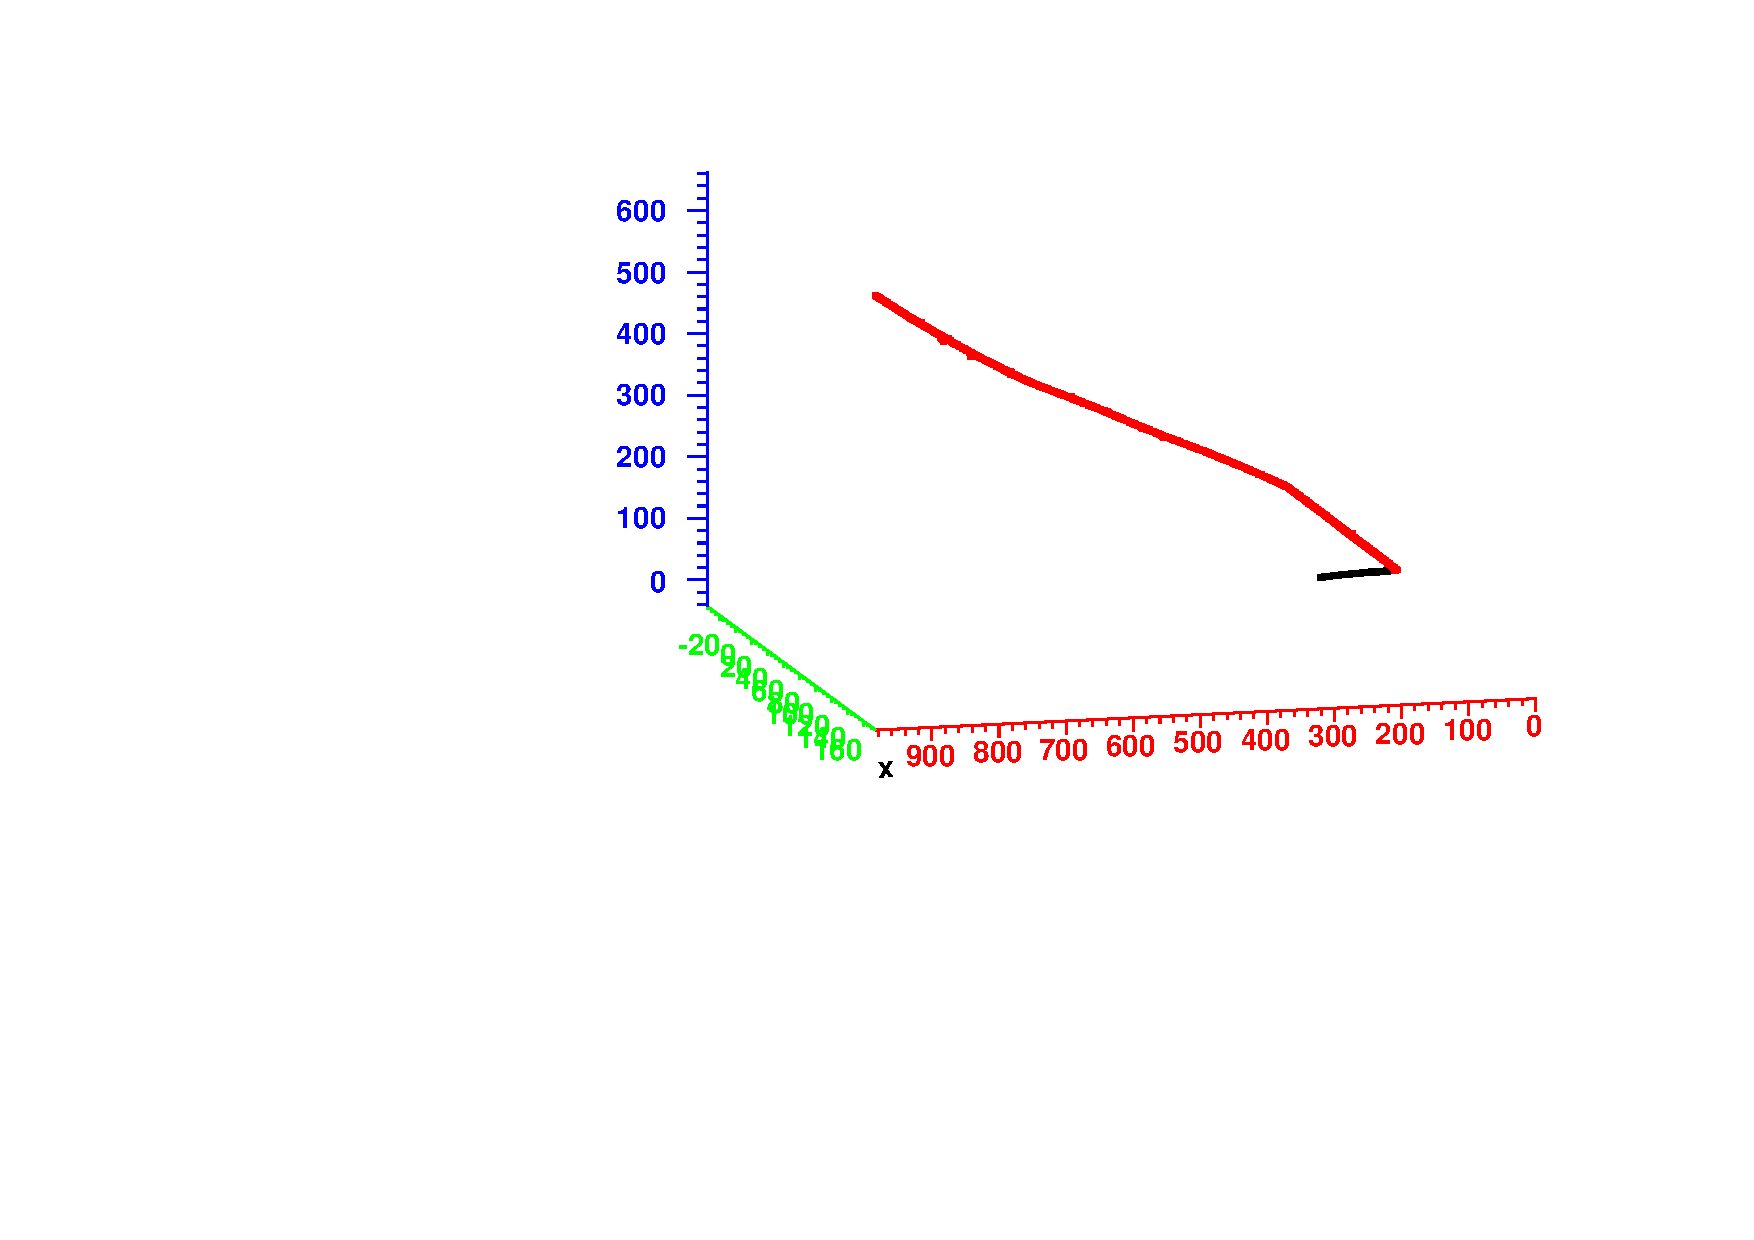
\includegraphics[angle=-90,width=0.6\textwidth]{chapters/cellularautomaton_images/event_8_2tr}
        \label{fig:ca-clusters-ccqe-2tr}
    }
    \subfigure[]{
        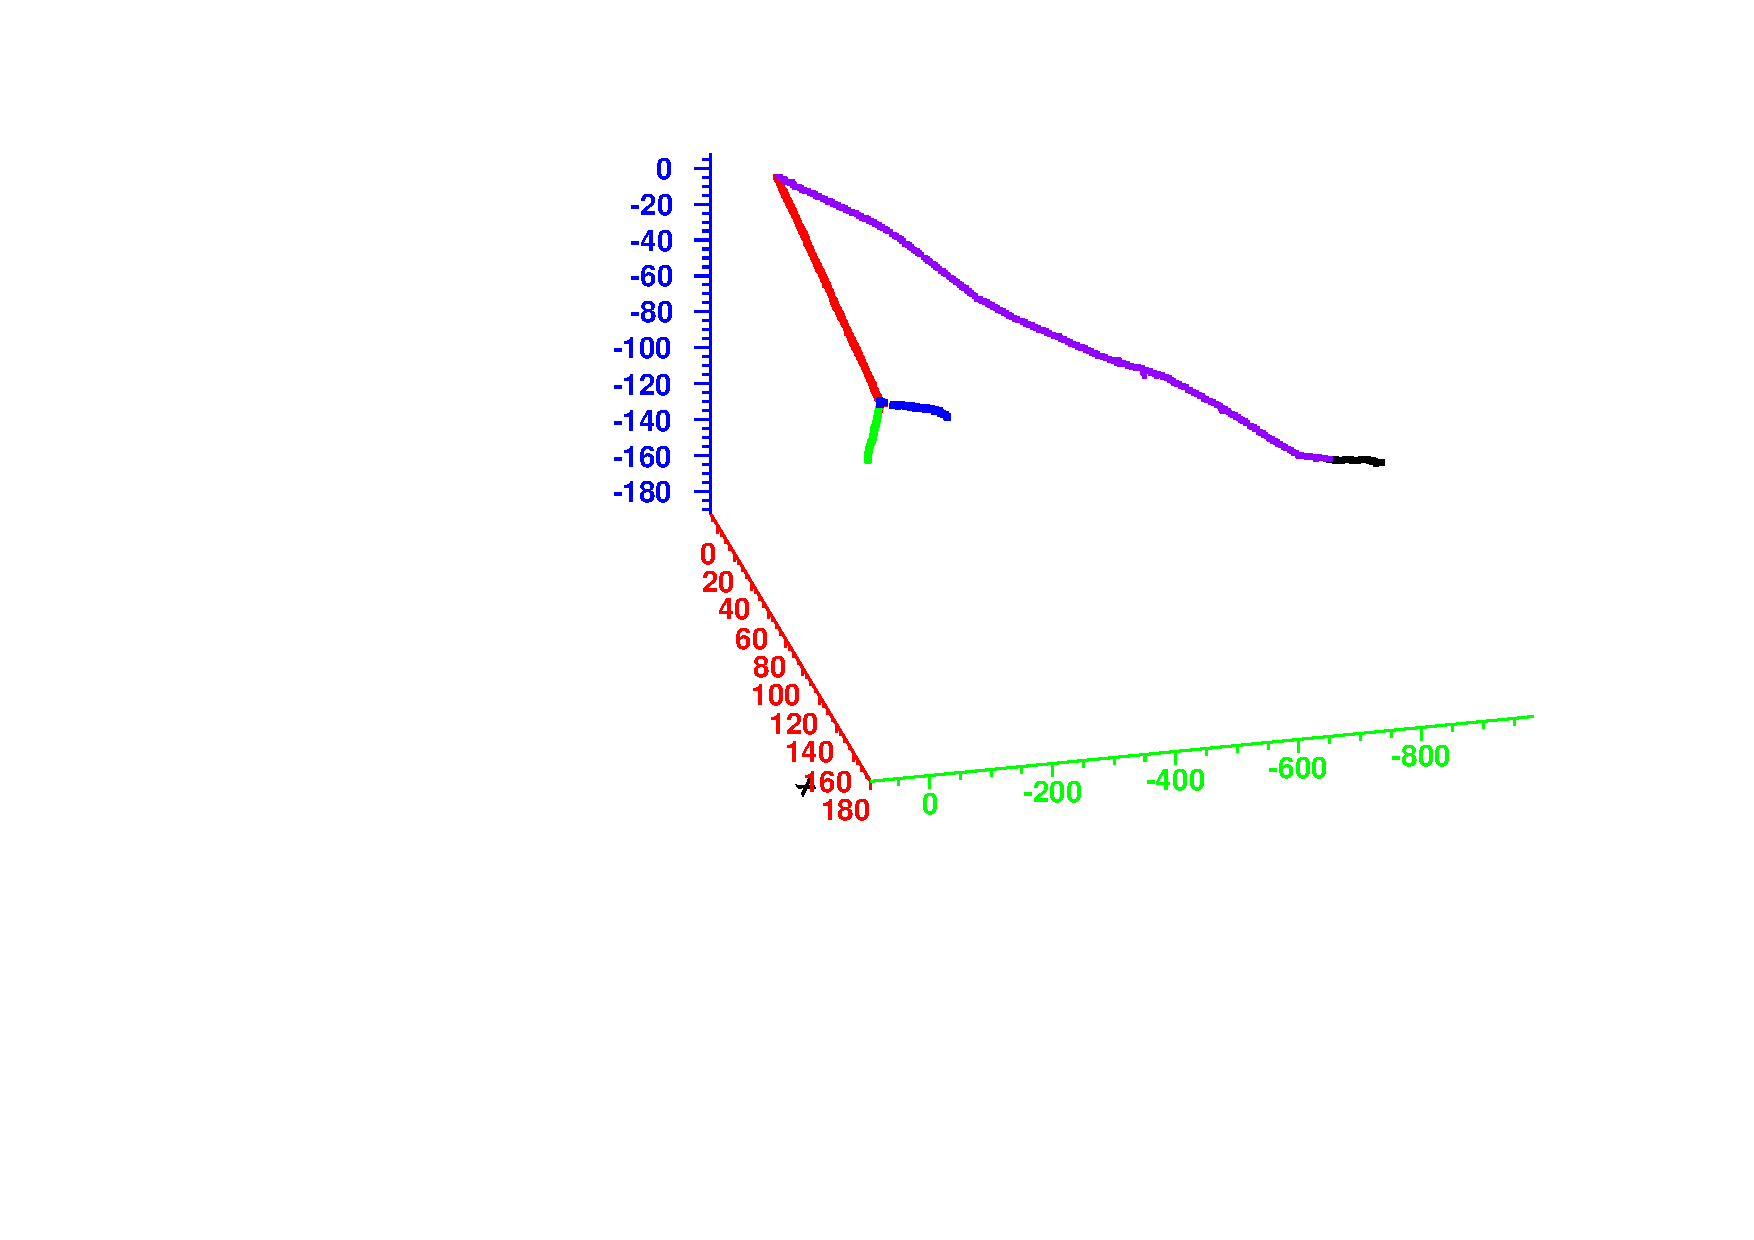
\includegraphics[angle=-90,width=0.6\textwidth]{chapters/cellularautomaton_images/event_366_mu_decay_p_hadronic}
        \label{fig:ca-clusters-ccqe-decay}
    }
    \subfigure[]{
        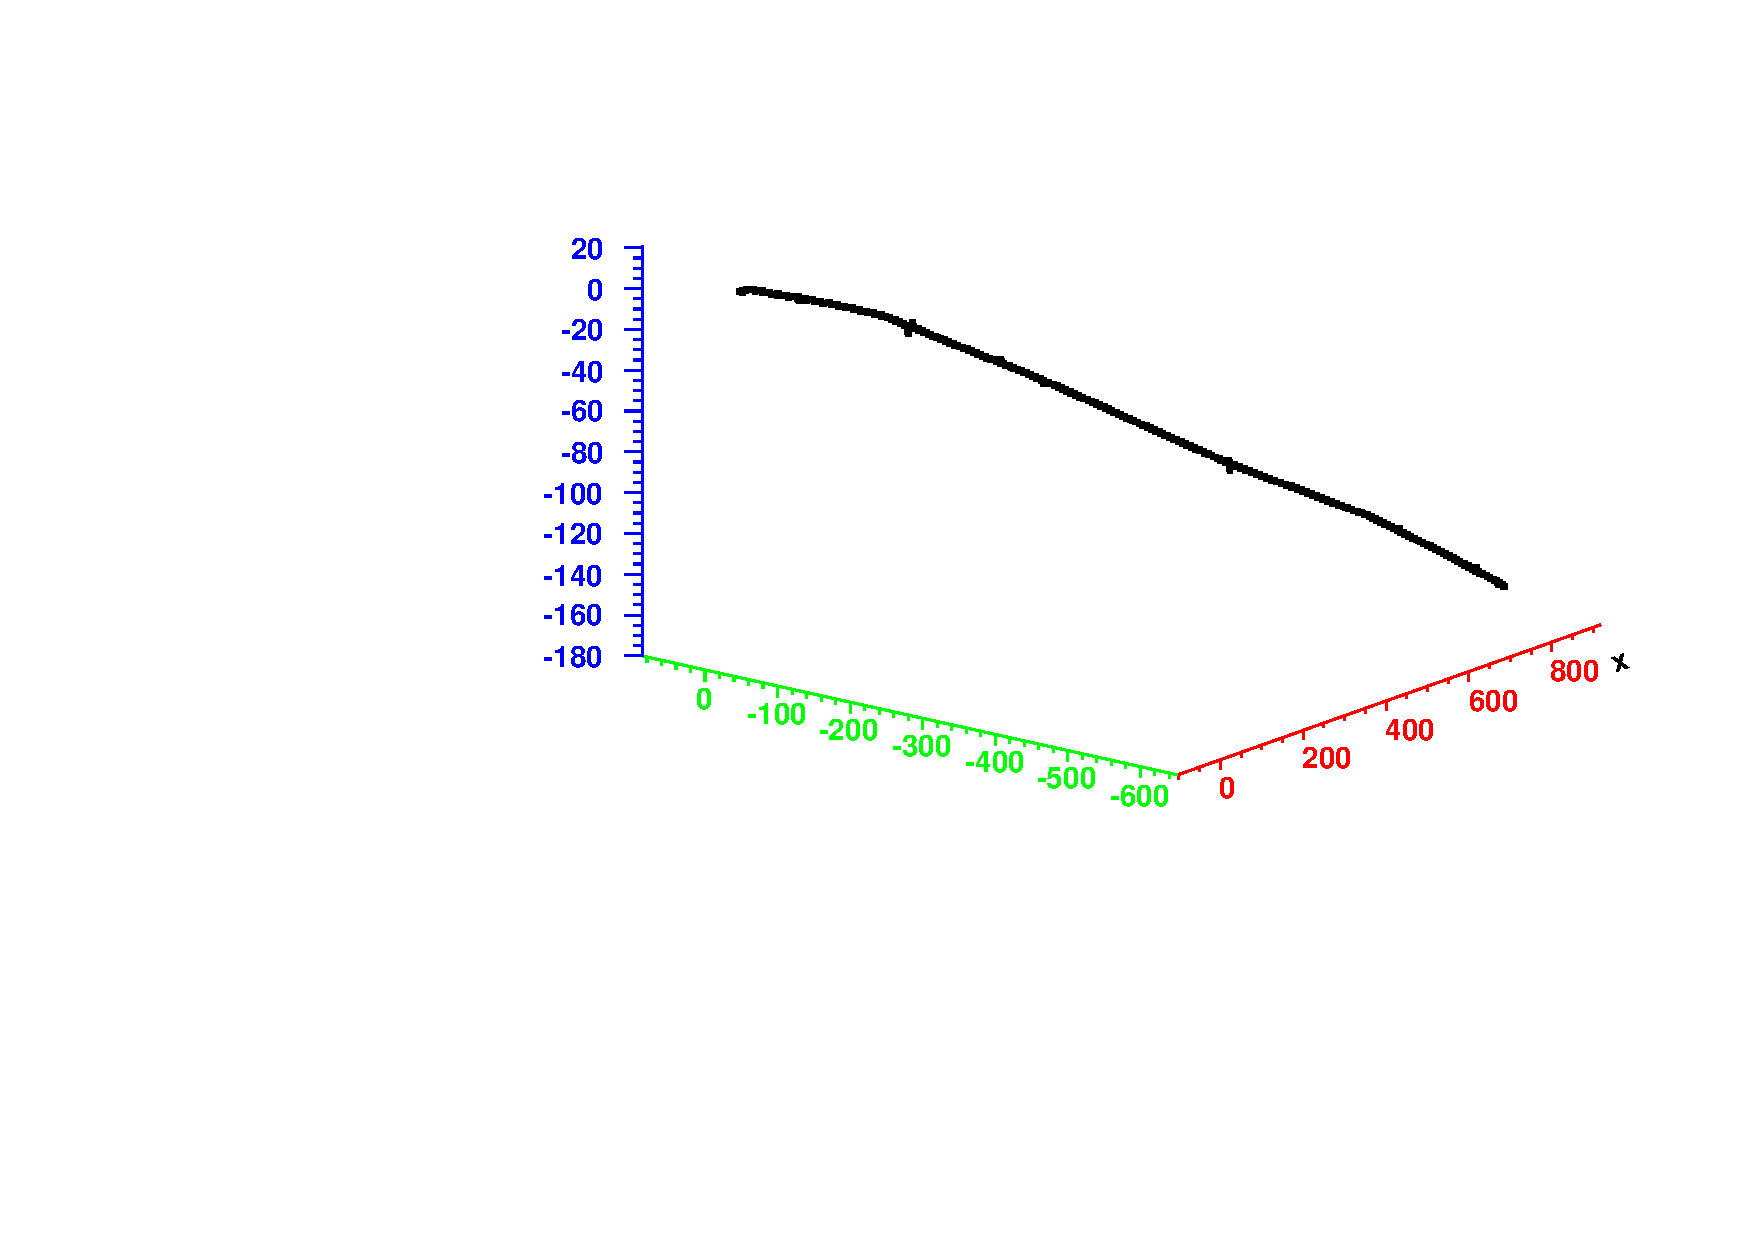
\includegraphics[angle=-90,width=0.6\textwidth]{chapters/cellularautomaton_images/event_986_1tr}
        \label{fig:ca-clusters-ccqe-1tr}
    }
    \caption[Clusters found by the CA in $\ccqe$ events]{\label{fig:ca-clusters-ccqe}Clusters found by the CA in $\nu_\mu$ charged current interactions resulting in $\ccqe$ final states. \subref{fig:ca-clusters-ccqe-2tr} $\mu$ (red) and proton (black) tracks correctly clustered. \subref{fig:ca-clusters-ccqe-decay} $\mu$ track (purple) and Michel electron (black), proton (red) and products of hadronic reinteraction (blue, green). \subref{fig:ca-clusters-ccqe-1tr} an event in which the $\mu$ and proton were produced with nearly identical trajectories and the CA was only able to find one track. Axes are labelled in $\mm$.}
\end{figure}

\begin{figure}
    \centering
    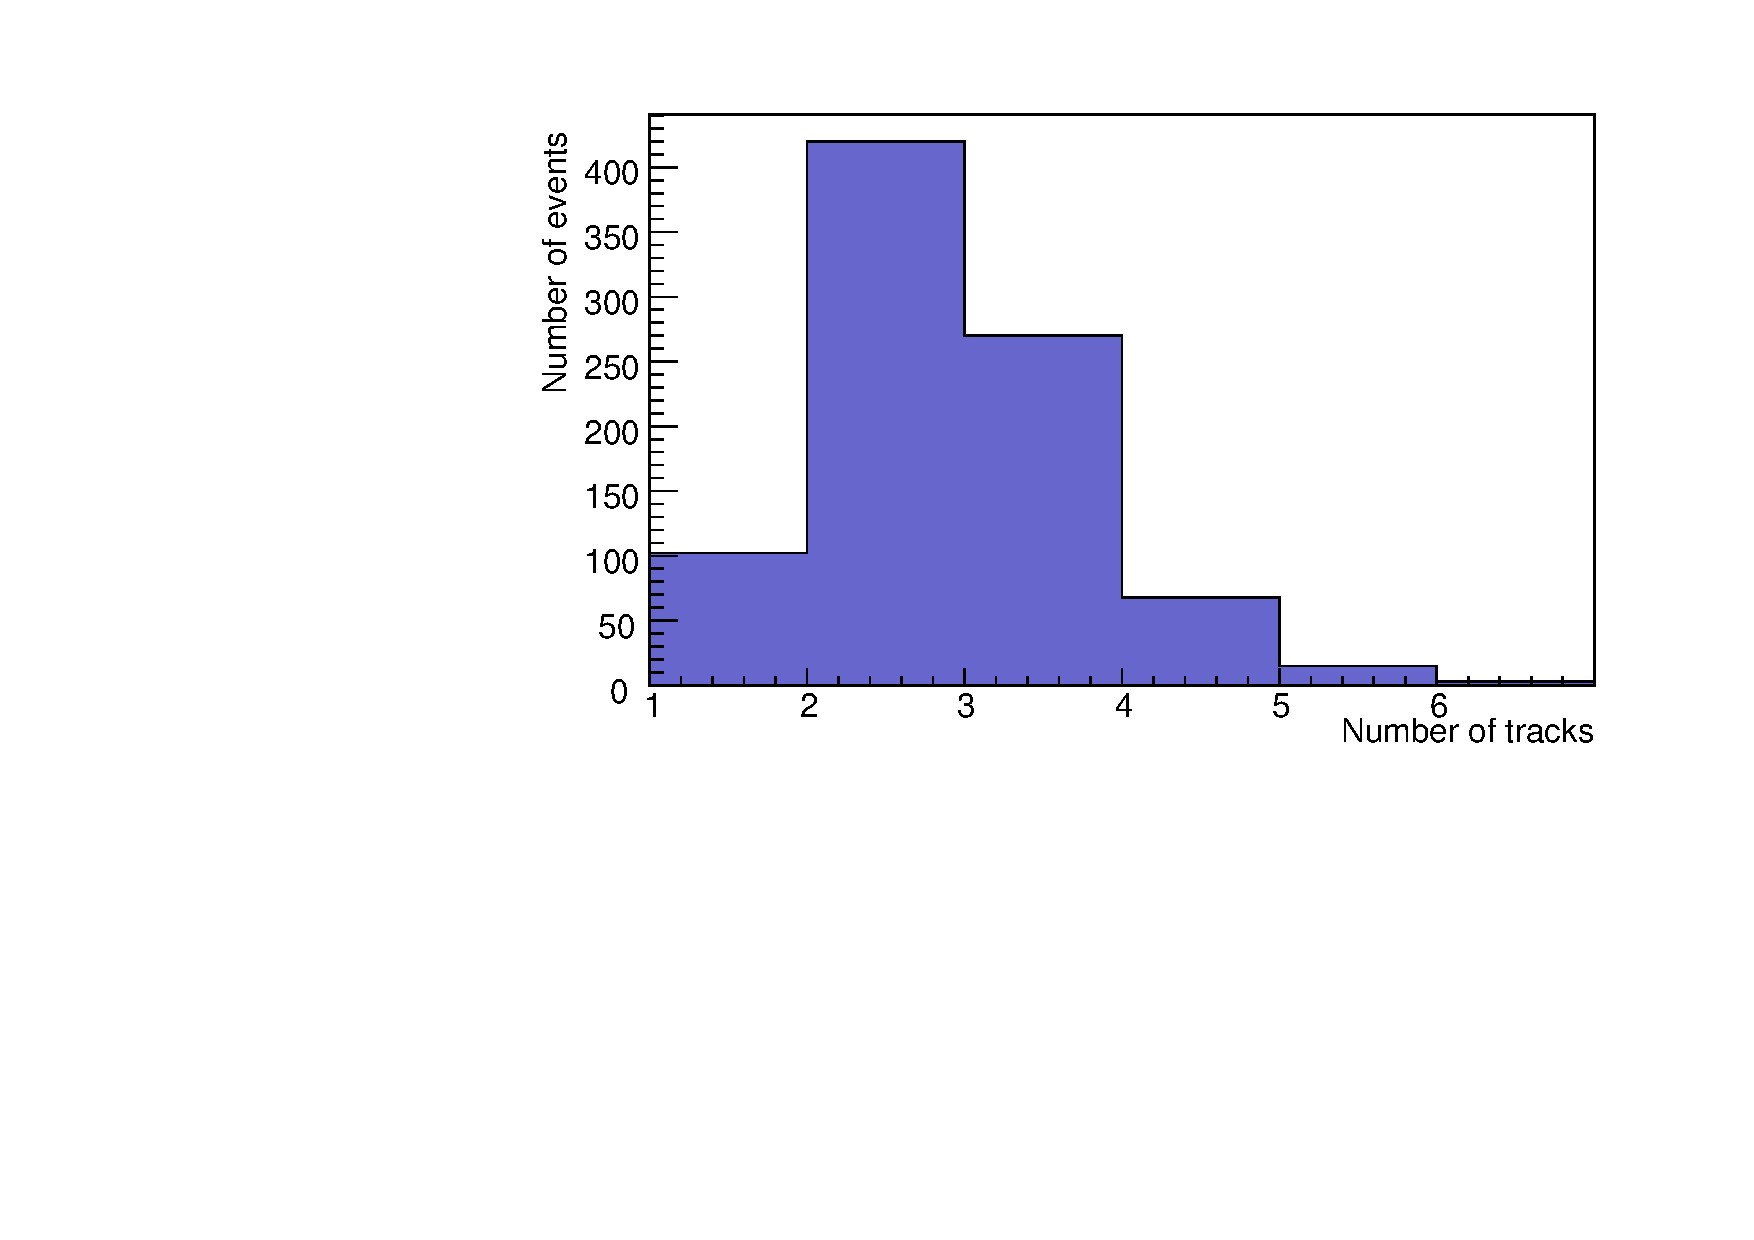
\includegraphics[angle=-90,width=0.8\textwidth]{chapters/cellularautomaton_images/ccqe-trackcount}
    \caption[Number of reconstructed tracks in CCQE events]{\label{fig:ca-ccqe-full-trackcounts}Distribution of reconstructed track counts for CCQE $\nu_\mu$ interactions resulting in $\ccqe$ final states, including hits from secondary particles. Events with a proton track of more than 20 hits were processed, and any trajectory of more than 20 hits was included in the input data. The expectation is to reconstruct two or more tracks (lower numbers are better). 878 events passed the range cut, of which approximately $11\%$ fall into the one-track bin here. The reconstruction can therefore be said to be $89\%$ efficient.}
\end{figure}

\begin{figure}
    \centering
    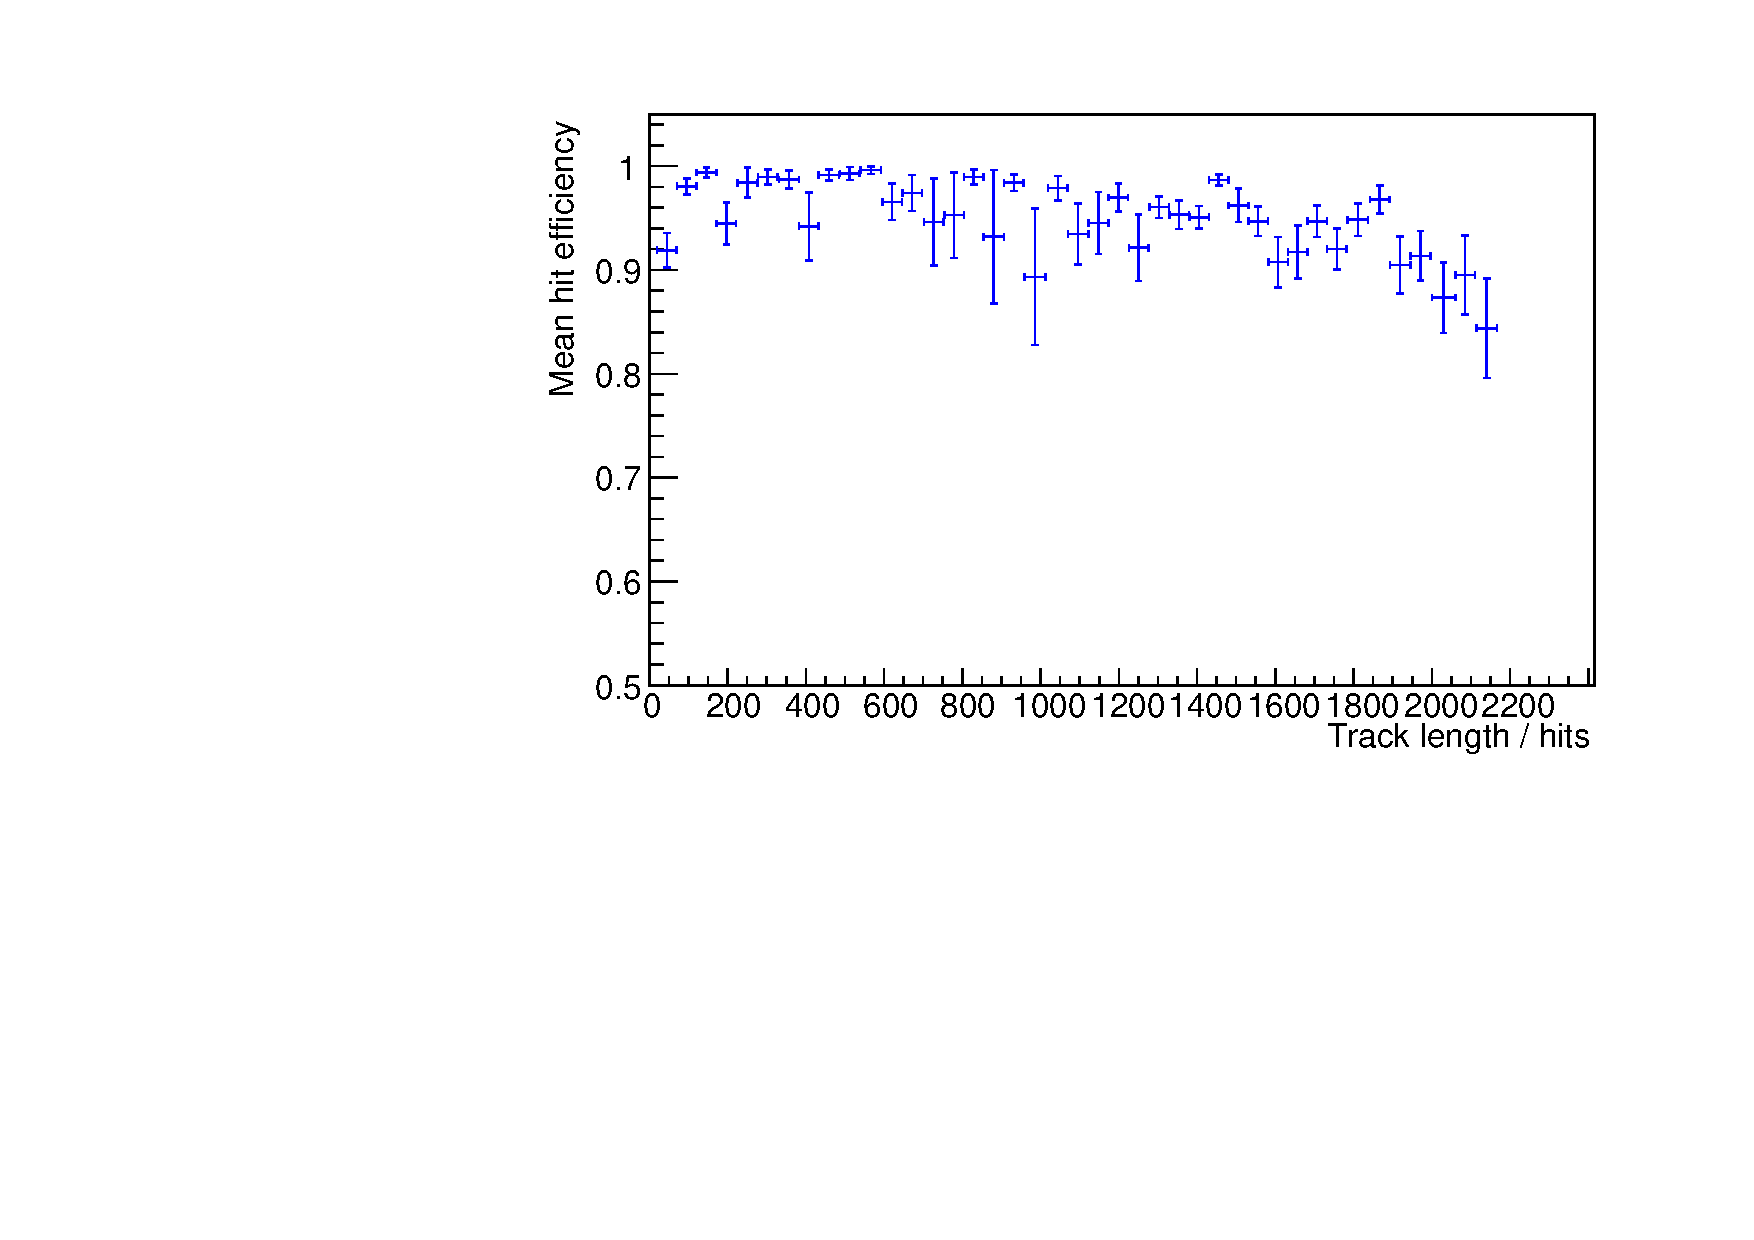
\includegraphics[angle=-90,width=0.8\textwidth]{chapters/cellularautomaton_images/ccqe-efficiency}
    \caption[Hit efficiency for CCQE events reconstructed with a CA]{\label{fig:ca-ccqe-full-efficiency}The hit efficiency (number of hits from the input that remain in an output cluster) for the CA operating on CCQE $\nu_\mu$ interactions with a $\ccqe$ final state. The efficiency is high for all truth track lengths, though the reduction in efficiency towards longer tracks remains.}
\end{figure}

\begin{figure}
    \centering
    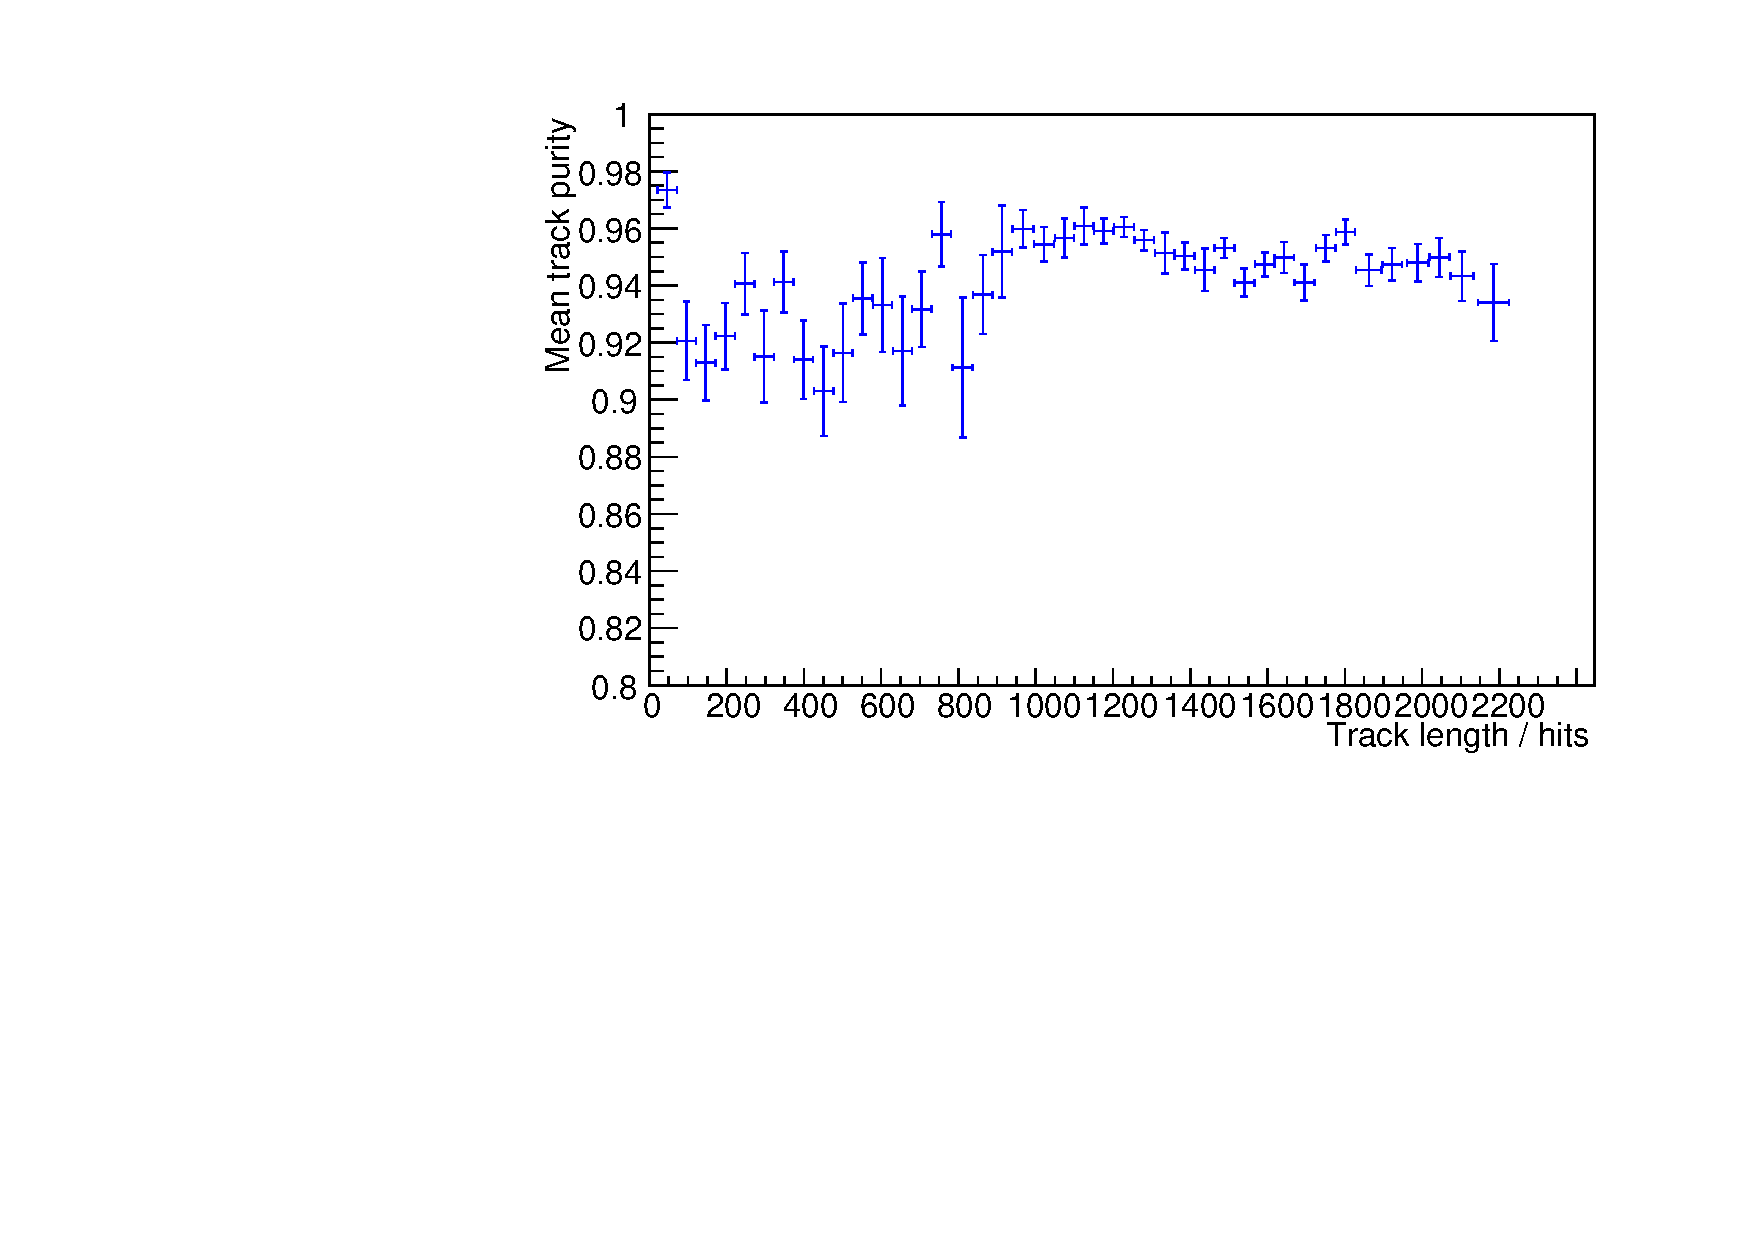
\includegraphics[angle=-90,width=0.8\textwidth]{chapters/cellularautomaton_images/ccqe-purity}
    \caption[Track purity for CCQE events reconstructed with a CA]{\label{fig:ca-ccqe-full-purity}The track purity (fraction of hits within a cluster that originate from the same truth track) for the CA operating on CCQE $\nu_\mu$ interactions with a $\ccqe$ final state. The purity is high for all cluster lengths.}
\end{figure}

Figure \ref{fig:ca-ccqe-full-efficiency} shows the hit efficiency (as defined above) for the full CCQE reconstruction. Here, the drop in efficiency with increasing track length is still present, though the effect is reduced; probably because the additional hits from delta electrons help to smooth out the large scattering angles sometimes present, and allow the \ac{CA} to run through them. Figure \ref{fig:ca-ccqe-full-purity} demonstrates that the \ac{CA} produces extremely pure tracks (over $90\%$ pure) even in situations where hits from delta electrons, decay products and other sources of noise are present. Since one of the main goals of clustering is to obtain collections of related hits, a high purity is very important.

\subsection{Charged Current $\nu_\mu \rightarrow \ccpi$ ($\CCPI$)}
A small fraction of low energy neutrino charged current interactions will produce a charged pion in the final state, mostly through the production and subsequent decay of nucleon resonances. These events were generated with Genie, taking all charged current interactions at the required energy of $0.77\GeV$ and selecting those with a $\ccpi$ (only) final state. The reconstruction algorithm parameters were identical to those applied to the \ac{CCQE} events, above, i.e. $\theta=10\degree$, $R_w=5.0\mm$ and $R_m=30.0\mm$. Once again, 1000 events were generated, and a range cut of 20 hits imposed on both the proton and pion tracks, leaving 891 events for reconstruction.

In principle, the task of reconstruction is more challenging for these events due to the additional final state particle when compared to the CCQE events. In practice, the \ac{CA} handles these events with little degradation of performance. Figure \ref{fig:ca-ccpi-trackcounts} shows the distribution of number of tracks reconstructed. More tracks are found, on average, than in the CCQE events, which is to be expected since we must now consider the additional primary particle, decay products from the $\mu$ or $\pi^+$, and delta electrons or hadronic reinteraction of the proton, as before. Only 26 tracks ($3\%$) were reconstructed with fewer than three tracks. The \ac{CA} therefore successfully clusters $97\%$ of these events. Figure \ref{fig:ca-clusters-ccpi} shows an example of the CA output for a $\ccpi$ event in which both the $\mu$ and $\pi^+$ decay.

\begin{figure}
    \centering
    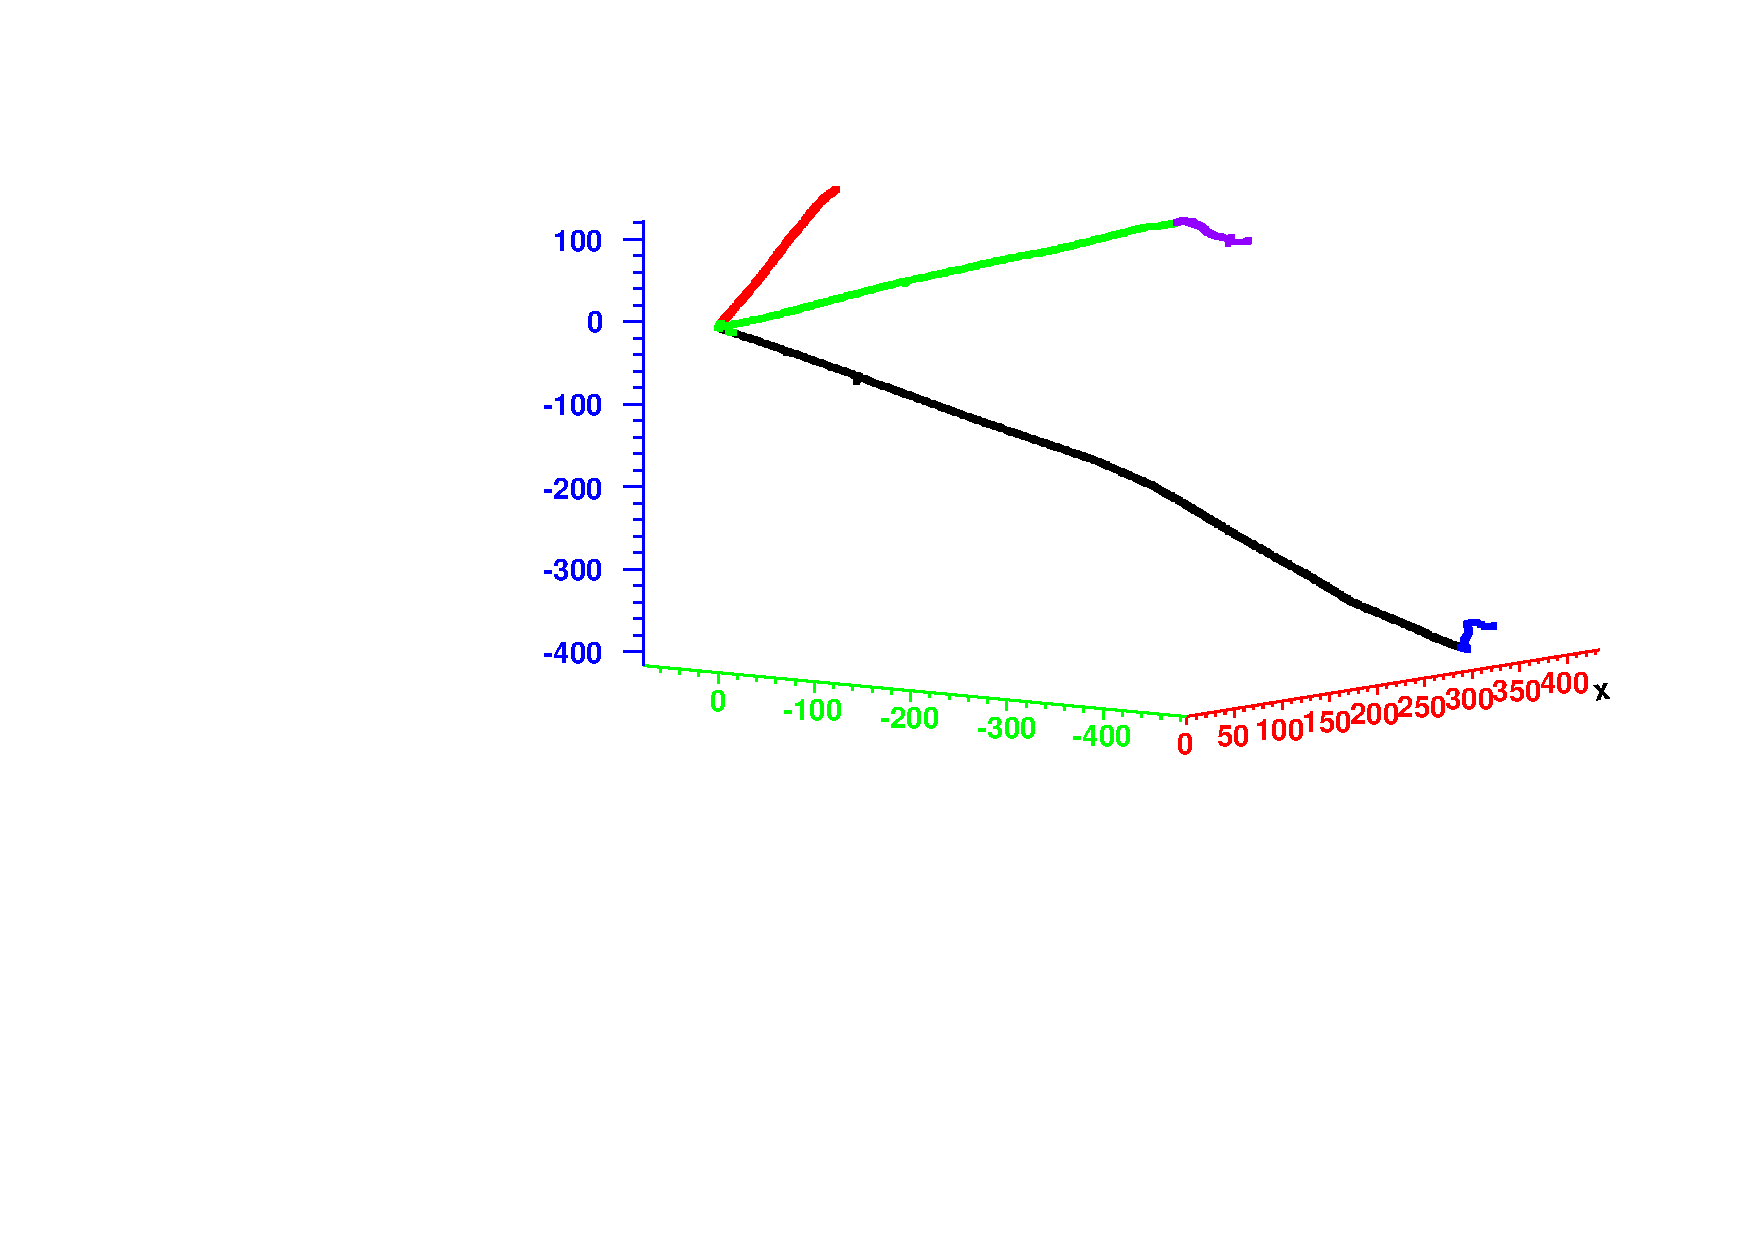
\includegraphics[angle=-90,width=0.7\textwidth]{chapters/cellularautomaton_images/ccpi_bothdecay}
    \caption[Clusters found by the CA in a $\ccpi$ event]{\label{fig:ca-clusters-ccpi}Clusters found by the CA for a charged current $\nu_\mu$ interaction resulting in a $\ccpi$ final state. The $\mu$ and $\pi^+$ both decay within the detector volume, and the CA produces one cluster for each major particle in the event; proton (red), $\pi^+$ (green) and its decay product (purple), the $\mu$ (black) and its Michel electron (blue). Axes are labelled in $\mm$.}
\end{figure}

\begin{figure}
    \centering
    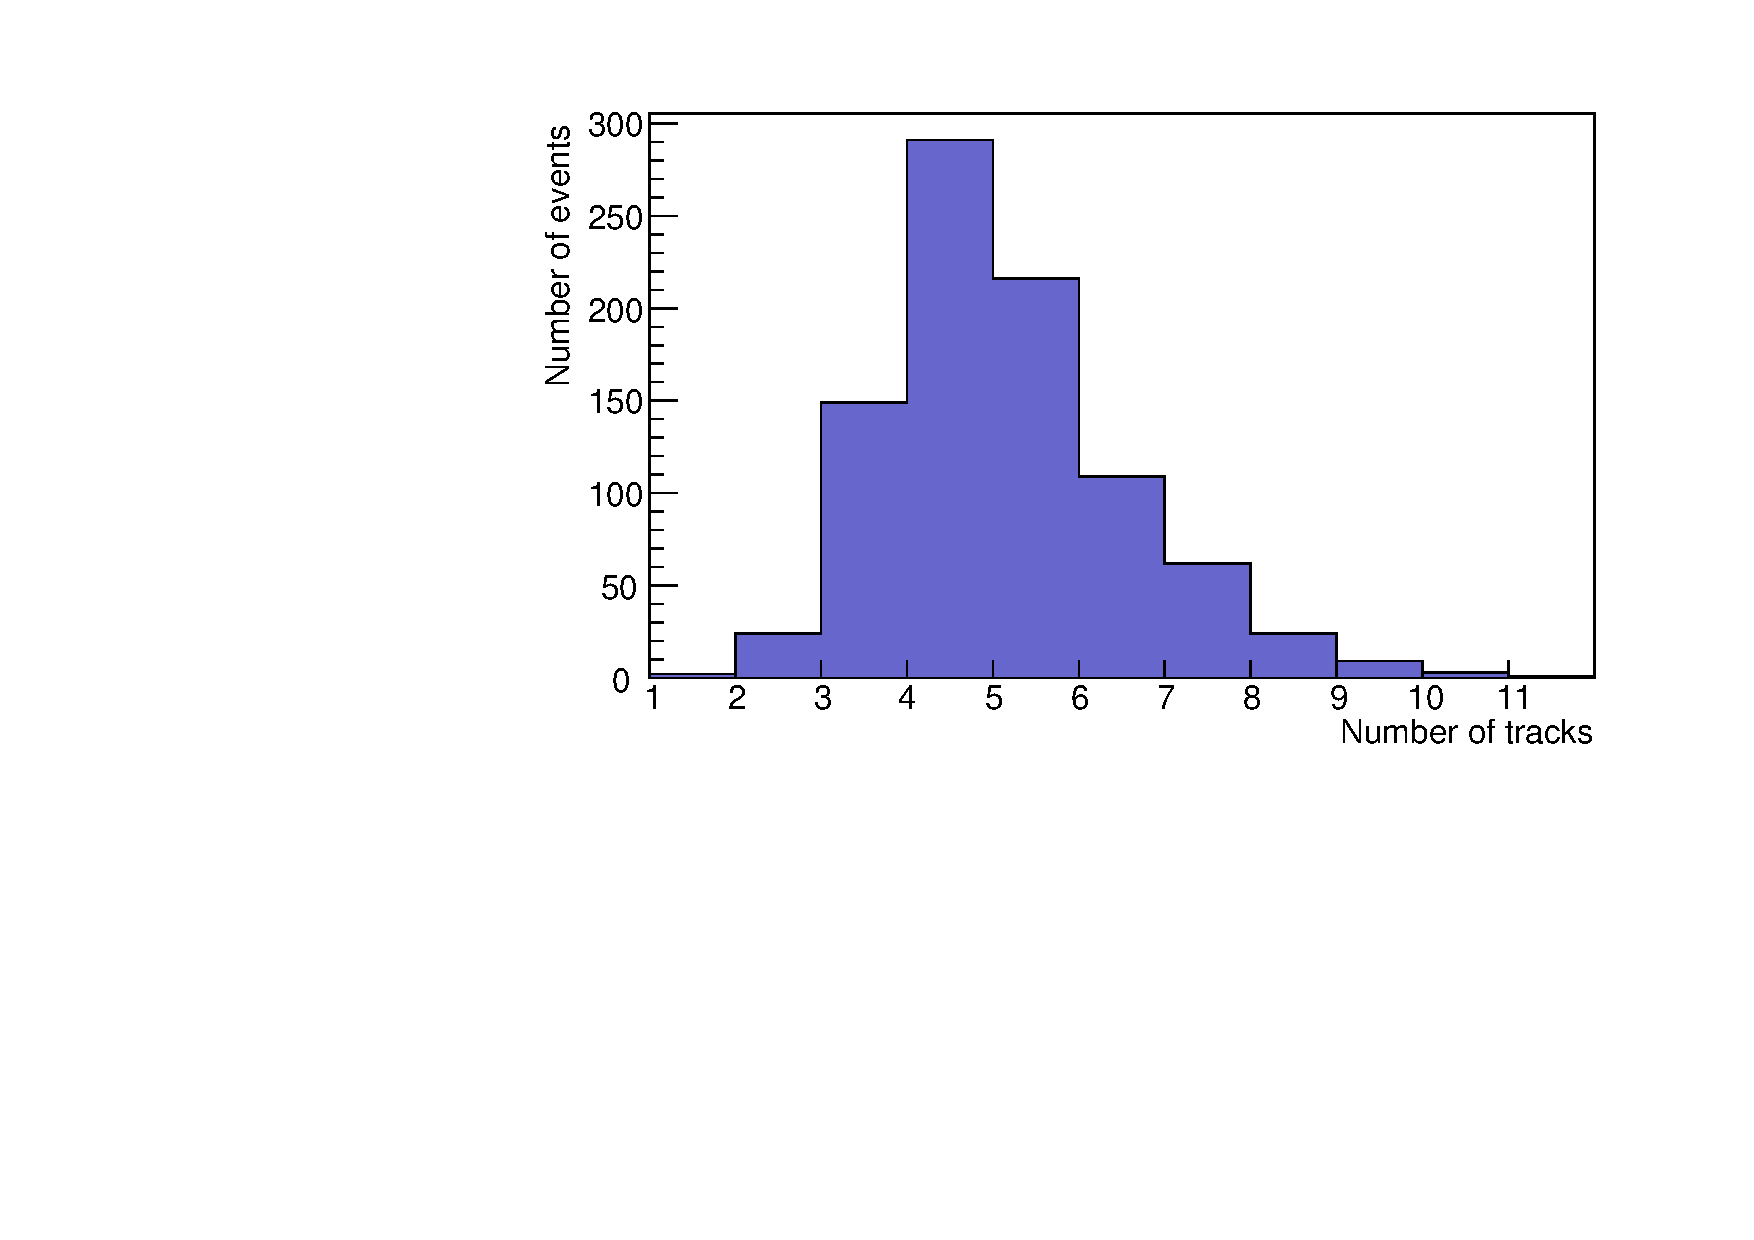
\includegraphics[angle=-90,width=0.8\textwidth]{chapters/cellularautomaton_images/ccpi-trackcounts}
    \caption[Number of reconstructed tracks in \acs{CCPi} events]{\label{fig:ca-ccpi-trackcounts}Distribution of reconstructed track counts for charged current $\nu_\mu$ interactions resulting in $\ccpi$ final states, including hits from secondary particles. Events with both proton and pion tracks containing more than 20 hits each were processed, and any trajectory of more than 20 hits was included in the input data. The expectation is to reconstruct at least three tracks, typically more. 891 events passed the range cut, of which approximately $3\%$ were reconstructed with fewer than three tracks.}
\end{figure}

\begin{figure}
    \centering
    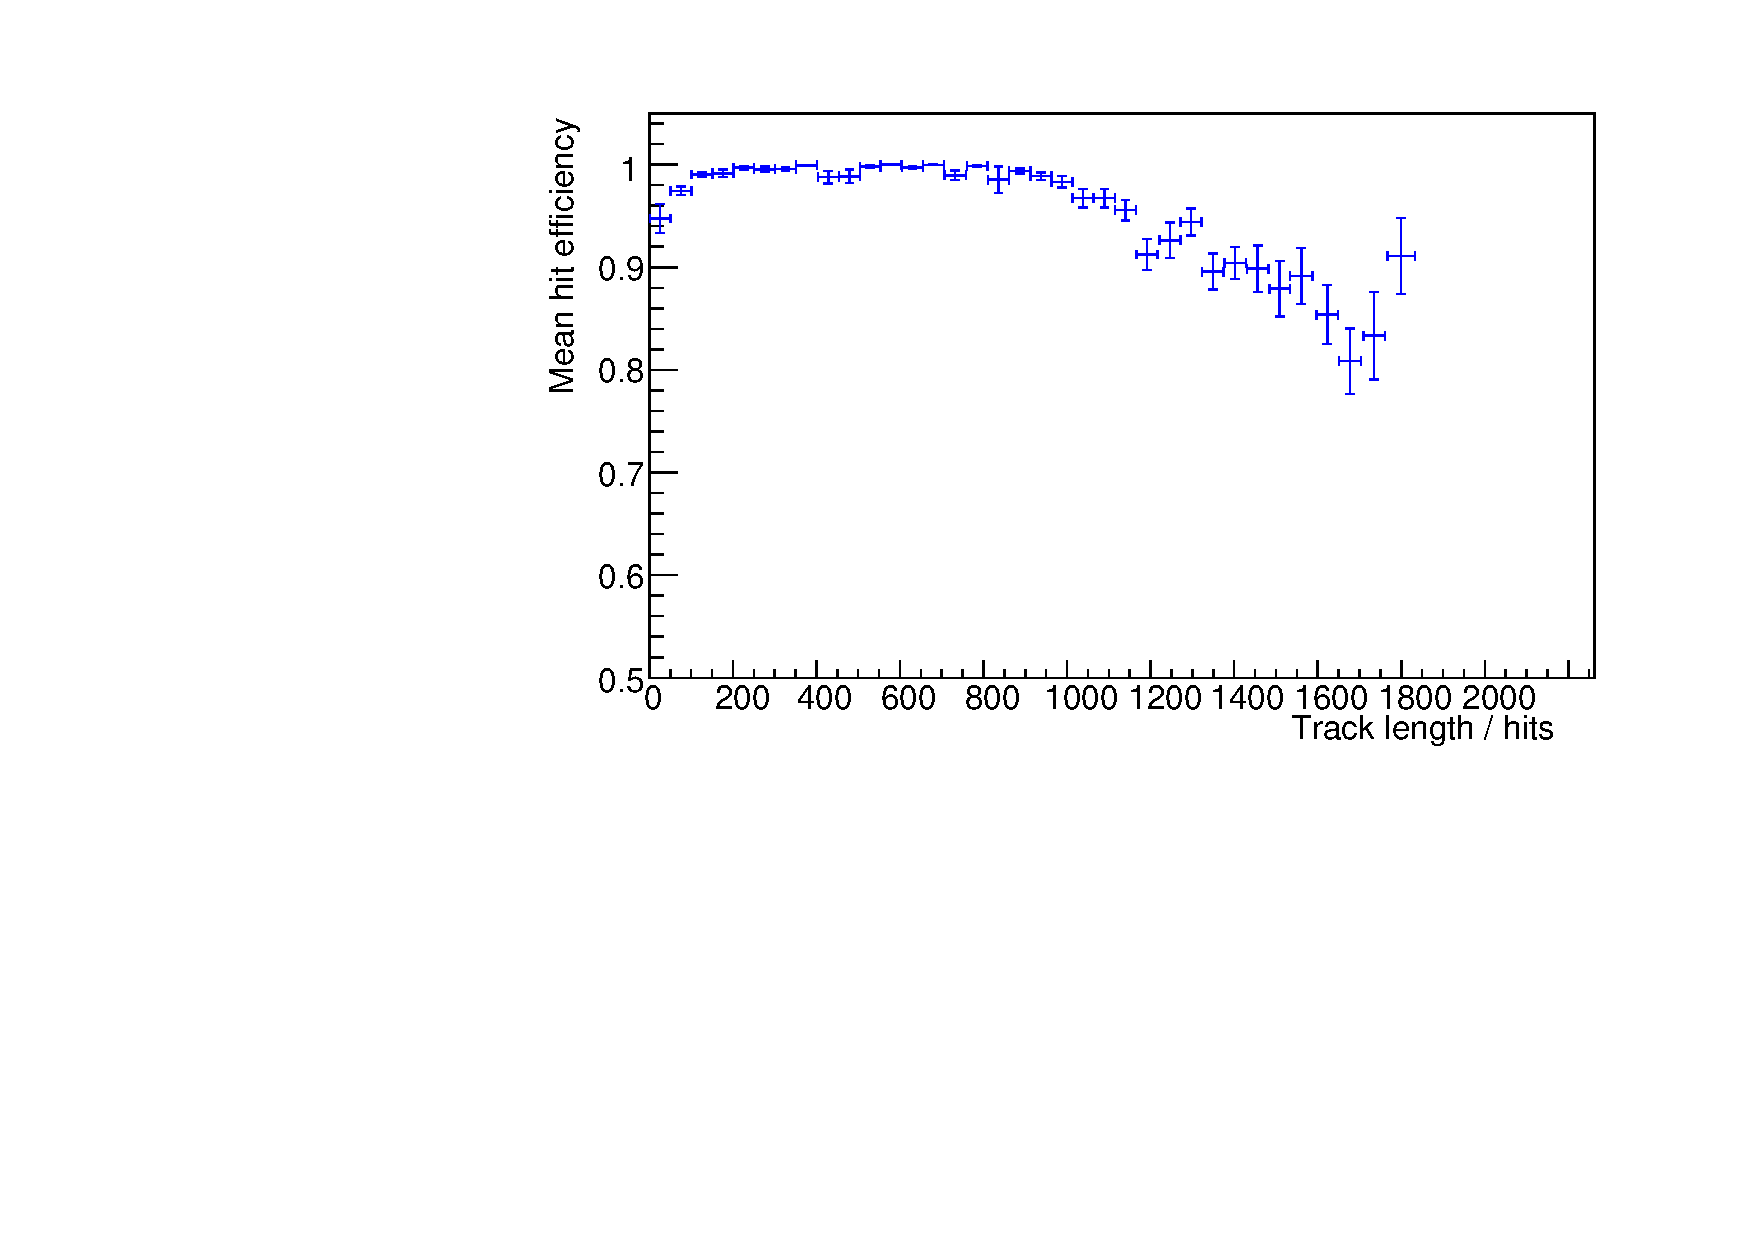
\includegraphics[angle=-90,width=0.8\textwidth]{chapters/cellularautomaton_images/ccpi-efficiency}
    \caption[Hit efficiency for \acs{CCPi} events reconstructed with a CA]{\label{fig:ca-ccpi-efficiency}The hit efficiency (number of hits from the input that remain in an output cluster) for the CA operating on $\nu_\mu$ charged current interactions with a $\ccpi$ final state. The efficiency is high for all track lengths, but exhibits the same decline with increasing track length as found in the CCQE reconstruction.}
\end{figure}

\begin{figure}
    \centering
    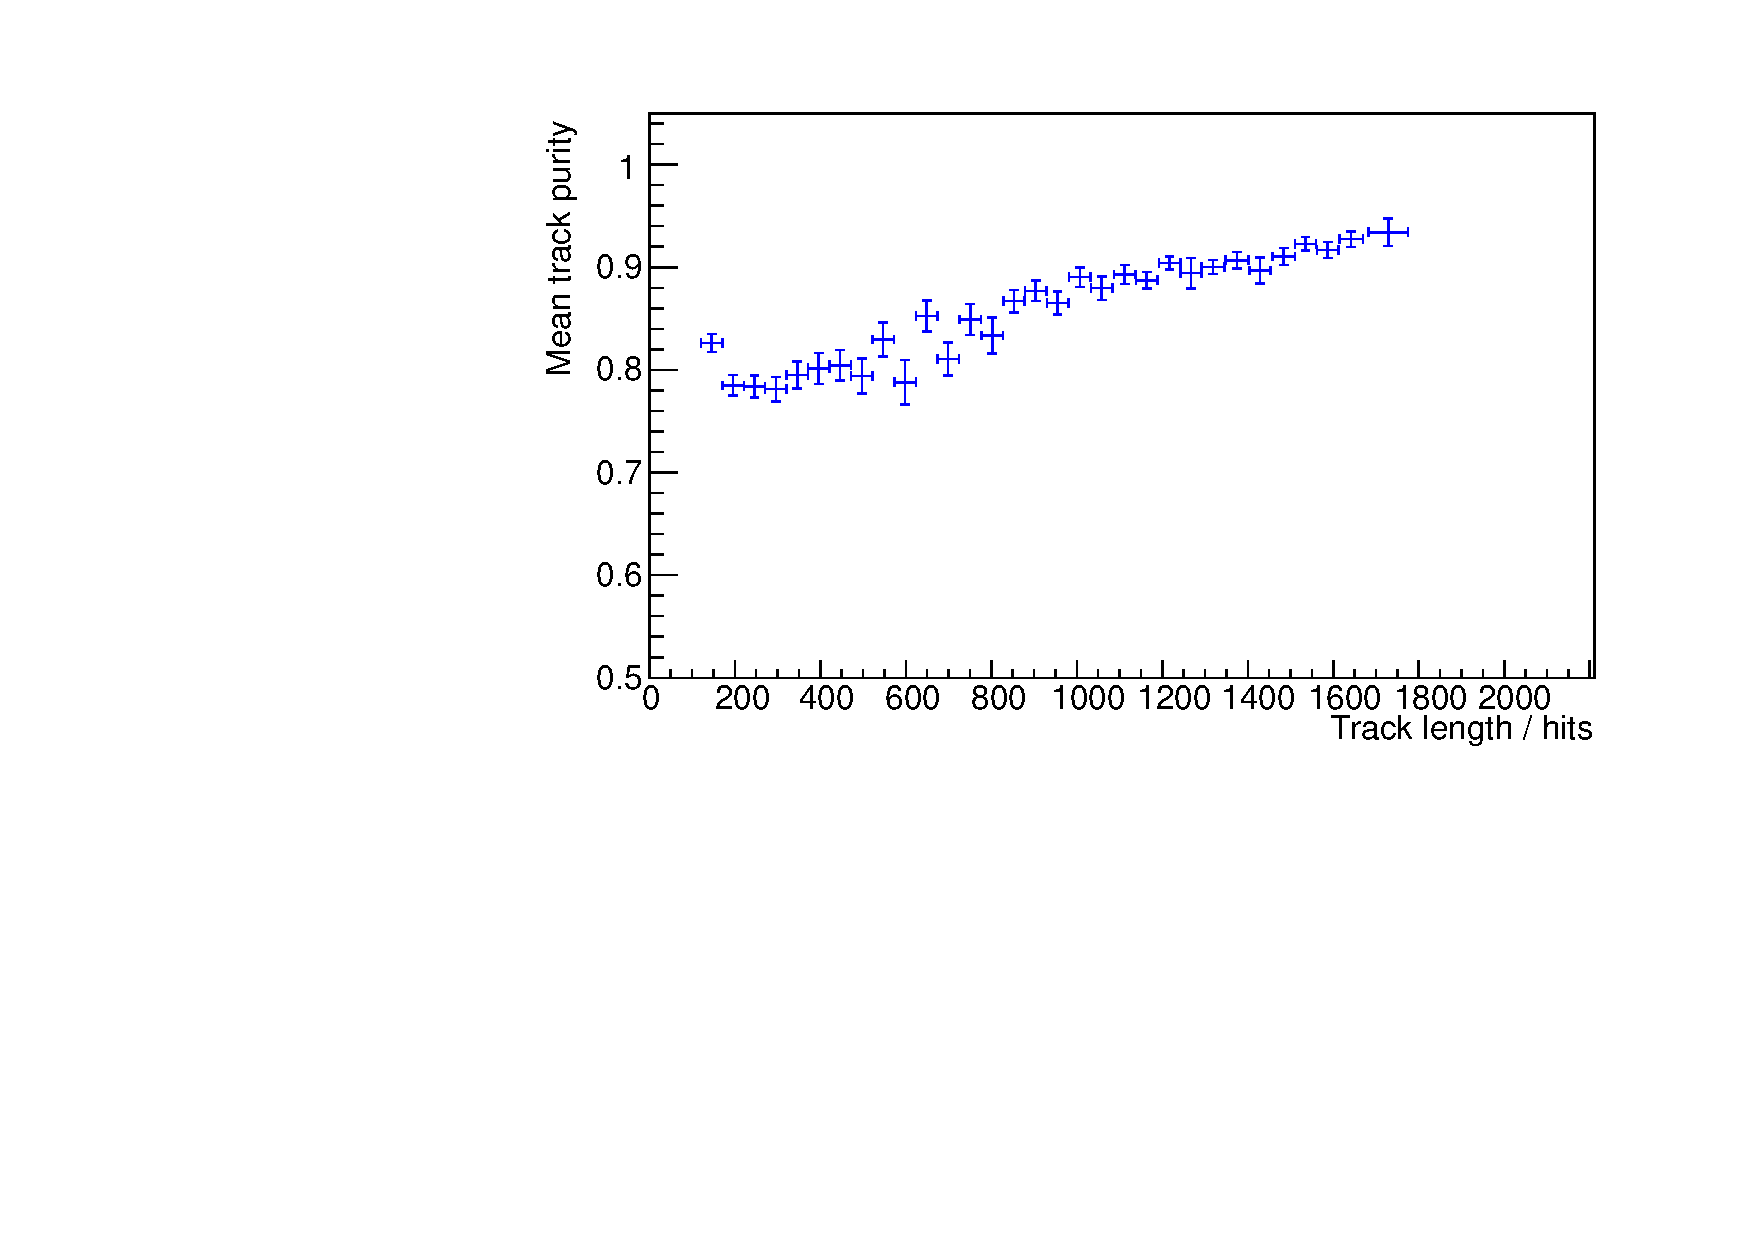
\includegraphics[angle=-90,width=0.8\textwidth]{chapters/cellularautomaton_images/ccpi-purity}
    \caption[Track purity for \acs{CCPi} events reconstructed with a CA]{\label{fig:ca-ccpi-purity}The track purity (fraction of hits within a cluster that originate from the same truth track) for the CA operating on $\nu_\mu$ charged current interactions with a $\ccpi$ final state. Short tracks exhibit low purity here, most likely because the addition of a final state $\pi^+$ means that the region around the neutrino interaction vertex is more densely populated than in the CCQE case. High purity is regained for longer tracks, i.e. away from the vertex along the $\mu$ track.}
\end{figure}

The hit efficiency (figure \ref{fig:ca-ccpi-efficiency}) for reconstruction of $\ccpi$ final states is high, but has the same characteristic tail-off with increasing track length. This reinforces the reasoning that the tail-off is due to large scattering events in the muon tracks as the particles deposit energy and slow down. The purity (figure \ref{fig:ca-ccpi-purity}) is lower than the CCQE case for short tracks, but this is expected because the region around the neutrino interaction vertex is more densely populated, making it harder for the CA to correctly cluster the hits. Further out, away from these sources of noise, the CA performs as well as in the CCQE case, and the purities of long tracks in \acs{CCPi} events are comparable to those from the CCQE events.

\section{Conclusions}
The \ac{CA} performs three-dimensional clustering with high efficiency, resulting in clusters of high purity (typically over $90\%$). There are a number of parameters that affect the operation of the algorithm, and these must, to an extent, be tuned to the particular application; for example the parameters providing optimal results for clean straight tracks differ from those used to reconstruct noisy physics tracks. The resulting clusters typically require further processing, such as merging and track fitting, but as a tool for hit association, the CA performs well when applied to the typical \ac{LAr TPC} data with high hit densities.

Most of the inefficiencies have topological causes; typically large angular deviations from straight lines, or a high density of tracks close to a vertex, both of which reduce the ability of the CA to produce a small number of pure clusters. Much of this inefficiency could be recovered by applying other algorithms, such as the feature detection algorithm of chapter \ref{sec:latte_feature_detection} to locate interaction and decay vertices, then removing hits in a small sphere around those features. This would leave simpler line-like objects for the CA to work with. Another approach might be to explicitly include the charge deposits as an additional `coordinate', linking together only those cells that form a consistent ionisation energy loss profile.

The CA could be used as part of a larger reconstruction package not only to find and cluster tracks, but also to remove track-like objects prior to shower characterisation and analysis. The identification and analysis of electromagnetic and hadronic showers is an important goal for software reconstruction of events in LAr TPCs, where it is complicated by the homogeneous nature of the detector allowing tracks and showers to develop alongside each other.

In conclusion, the use of a cellular automaton to perform three-dimensional reconstruction of tracks in liquid Argon data is a useful addition to the current knowledge base surrounding \ac{LAr TPC} reconstruction, and is particularly powerful when used as part of an integrated reconstruction package, where its inefficiencies can be compensated with other algorithms.
